\documentclass[conference]{IEEEtran}
\usepackage[utf8]{inputenc}
\usepackage[spanish]{babel}
\usepackage{enumerate}
\usepackage{graphicx}
\usepackage[colorlinks]{hyperref}
\usepackage{amssymb}
\usepackage{amsmath}
\usepackage{booktabs}
\usepackage{graphicx}
%Necesario para el parametro H en las figuras 
\usepackage{float}
% Numeros periodicos
\usepackage{yhmath}
\usepackage{fontawesome5}
\usepackage{csquotes} %Relación con el idimoa
\usepackage[backend=biber, style=ieee]{biblatex}
\usepackage{xr}
\usepackage{cuted}
\usepackage{caption}
\usepackage{enumitem}
\externaldocument{suplemento}

%\renewcommand{\tablename}{Tabla}
\captionsetup[table]{name=Tabla} 
\newcommand{\jph}[1]{{\color{blue}{#1}}}

\bibliography{Referencias}

\begin{document}

\title{Sistema de navegación adaptativa para un vehículo autónomo en un entorno con establecimiento objetivo}

\author{\IEEEauthorblockN{1\textsuperscript{er} Over Alexander Mejia Rosado \textsuperscript{\href{https://orcid.org/0009-0008-8152-2754}{\faOrcid}}}
\IEEEauthorblockA{\textit{Inteligencia Artificial} \\
\textit{Universidad Nacional de Colombia - De La Paz}\\
San Diego
}
\and
\IEEEauthorblockN{2\textsuperscript{do} Ronald Mateo Ceballos Lozano \textsuperscript{\href{mailto:rceballosl@unal.edu.co}{\faIcon{envelope}}}}
\IEEEauthorblockA{\textit{Inteligencia Artificial} \\
\textit{Universidad Nacional de Colombia - De La Paz}\\
Valledupar
}
\and
\IEEEauthorblockN{3\textsuperscript{er} Rhonald José Torres Diaz \textsuperscript{\href{mailto:rhtorresd@unal.edu.co}{\faIcon{envelope}}}}
\IEEEauthorblockA{\textit{Inteligencia Artificial} \\
\textit{Universidad Nacional de Colombia - De La Paz}\\
Valledupar
}}

\maketitle

\begin{strip}
\section*{Resumen}
Este proyecto se centra en el desarrollo de un sistema de navegación para vehículos autónomos utilizando NEAT (NeuroEvolution of Augmenting Topologies). El objetivo principal es diseñar e implementar un vehículo capaz de desplazarse en un mapa en 2D, el cual consta de un punto inical y un objetivo para el vehiculo autonomo. A través de sensores virtuales, el vehículo es capaz de identificar la vía por la cual puede avanzar y cuales los los limites de esta. Se utilizan métricas de distancia como la Euclidiana, Manhattan y Chebyshev cómo sistema de recompensas, que constantemente calculan las posiciones de los agentes, entre más cercano esté el vehiculo del objetivo, su fitness incrementa, de esa manera se esttablece la función aptitud. Se crea y se implementa un sistema de refuerzo forzado, que permite al vehículo avanzar en caso de que su velocidad sea menor a 0.1, evitando así que el vehículo se estanque. Los resultados obtenidos muestran que el vehículo autónomo es capaz de desplazarse de manera autónoma en el mapa, aumentando su aptitud en cada generación dependiendo de la metrica de distancia utilizada.
\end{strip}

\section{Introducción}
Uno de los mayores problemas del transporte moderno es el alto indice de accidentes en el tránsito terrestre, la gran cantidad de trafico atribuida a factores como errores humanos, falla mecánicas y fenómenos naturales. 

De acuerdo con el estudio realizado por la Organización Mundial de la Salud (OMS) en 2023, entre 2010 y 2021 el número de vehículos a nivel mundial se duplicó, superando los mil millones \cite{Accidentes}. Este crecimiento ha contribuido a un incremento en los accidentes de tránsito, que provocaron aproximadamente 1,19 millones de muertes en todo el mundo, con una tasa de mortalidad de 15 personas por cada 100,000 habitantes, lo que representa una disminución del 5\% en comparación con 2010. Además, cerca del 80\% de las vías de tránsito a nivel mundial no cumplen con los estándares básicos de seguridad para peatones y ciclistas. Esta falta de infraestructura segura expone a ciclistas y peatones a un alto riesgo de accidentes, especialmente en entornos urbanos con alta densidad de tráfico, lo que también genera congestión vehicular, alargando los tiempos de trayecto, incrementando las emisiones de gases contaminantes y provocando un desperdicio de combustible \cite{montezuma2008derecho, diaz2015infraestructuras}.

Estos factores resaltan la necesidad de intervenciones más efectivas, como la automatización y los sistemas inteligentes de tráfico, que permitan reducir las cifras de mortalidad y mejorar la eficiencia del tránsito mediante sistemas coordinados.

%Sistemas autonomonos
%\subsection{Sistemas Autónomos}
Con el continuo avance de las tecnologías emergentes, la implementación de vehículos autónomos pasó de ser un futuro cercano a un presente en constante evolución. Estos sistemas, mejoran la seguridad y eficiencia tanto del vehículo como del transporte en general, enfocándose no solo en el control preciso del automóvil, sino también en la capacidad del sistema para adaptarse dinámicamente a condiciones variables y mantener una trayectoria segura para los pasajeros y otros agentes viales \cite{arshad2020clothoid}. El control de movimiento y la precisión en el seguimiento de trayectoria son aspectos críticos para la evaluación del agente inteligente a bordo del vehículo, siempre con el objetivo de preservar la integridad de las personas dentro del automóvil. El control de movimiento en vehículos autónomos, en especial el control óptimo de seguimiento de trayectoria busca mantener al vehículo dentro de los limites de seguridad establecidos, optimizando los movimientos del automóvil y ajustando el comportamiento del vehículo a través de inteligencia artificial avanzada, como la ADP (Adaptive Dynamic Programming), o Approximate Dynamic Programming (Programación dinámica aproximada) \cite{ADP_A}. La ADP es una técnica de control avanzada utilizada en vehículos autónomos para la toma de decisiones en tiempo real bajo condiciones de incertidumbre, y con tecnología de control basada en el aprendizaje por refuerzo, el uso de programación dinámica adaptativa critica, aumenta el rendimiento del sistema \cite{Smart_Car_ADP, ADP_Inf}. La ADP utiliza una función de costo que evalúa el rendimiento del control del vehículo, minimizandose esta función mediante procesos iterativos, lo que le permite ajustar continuamente las acciones para optimizar el rendimiento y reducir errores de seguimiento en la trayectoria. En \cite{Smart_Car_ADP} se propone un método de control óptimo adaptativo con rendimiento prescrito para resolver el problema del control de seguimiento de trayectorias para vehículos autónomos con dinámica inercial, y al introducir una función de rendimiento prescrito (PPF) en la programación dinámica adaptativa (ADP), el controlador puede restringir el error de seguimiento del sistema dentro de un límite de rendimiento especificado al tiempo que optimiza el costo de control.


%El aprendizaje por refuerzo que ha demostrado ser eficaz en la toma de decisiones en vehículos autónomos es el Deep Q-Network (DQN). En este enfoque, el agente aprende a tomar decisiones a través de la interacción con su entorno, recibiendo recompensas o penalizaciones en función de sus acciones, lo que mejora su aprendizaje \cite{DQN_Inf}. La técnica DQN utiliza funciones que estiman el valor de las acciones en los diferentes estados en los que se encuentra el agente, representando así la expectativa de recompensa acumulada al realizar una acción específica desde un estado particular.

%Además, DQN implementa un balance entre exploración y explotación. La exploración implica probar nuevas acciones, mientras que la explotación se refiere a elegir acciones que el agente considera "buenas". Este balance se evalúa mediante el mecanismo epsilon-greedy, donde el agente elige acciones aleatorias con una probabilidad $\epsilon$ que varía entre 0 y 1 \cite{atari}. Un valor alto de $\epsilon$ permite una mayor exploración, mientras que un valor bajo indica una mayor explotación de las acciones ya aprendidas. Sin embargo, debido a que el operador máximo en DQN selecciona el valor máximo para evaluar una acción producida por el mismo valor Q, existe el riesgo de obtener valores estimados de manera demasiado optimista. Para mitigar este problema, se propone disociar la selección de la evaluación, lo que da lugar al enfoque Double DQN \cite{Double-DQN}. En este método, se utilizan dos funciones de valor (redes Q) que se aprenden actualizando alternativamente una de ellas, resultando en dos conjuntos de pesos de red: $w$ y \( w^{\prime} \). La función de valor con peso $w$ se utiliza para determinar la acción a tomar, de acuerdo con una política voraz, mientras que la función con peso \( w^{\prime} \) se utiliza para evaluar el valor Q.

%DQN puede ser implementado en los casos donde se requiera alta precisión,  cómo por ejemplo la construcción mapas. También aplicar el DQN en la conducción autónoma y el transporte inteligente, mejorando así la trazabilidad de las trayectorias en vehículos autónomos \cite{Smart_Car_DQN}.

%El Deep Deterministic Policy Gradient (DDPG), es otro algoritmo de aprendizaje por refuerzo diseñado para resolver problemas de control continuo, este dependiendo del entorno, puede aumentar la optimización del sistema, agregando un mayor indice de credibilidad al algoritmo \cite{movile}.
 
%Por otro lado se encuentra la PPO (Proximal Policy Optimization) una técnica de aprendizaje por refuerzo avanzada y popular utilizada en entornos complejos de sistemas de vehículos autónomos. La PPO pertenece a los métodos de optimización de políticas, lo que significa que se centra en las estrategias a seguir con respecto al entorno dinámico donde se encuentra el agente. Esta técnica introduce una optimización proximal para limitar cuanto se puede actualizar la política en cada paso de entrenamiento, limitando así los grandes cambios en las políticas y estabilizando el aprendizaje para que el agente sea consistente \cite{PPO_Inf}. A diferencia de los métodos basados en funciones Q, PPO aprende directamente una política estocástica, lo que significa que genera probabilidades para cada acción en lugar de seleccionar siempre la misma acción en un estado determinado. Este implementa un algoritmo $actor-critic$ donde el actor aprende la política (qué acción tomar en cada estado) y  el critic estima el valor de cada estado (cuál es la recompensa esperada en un estado dado). Esta técnica se ha utilizado en el siguiente articulo \cite{Smart_Car_PPO} donde se presento un enfoque basado en MAPPO (Multi-Agent Proximal Policy Optimization) para garantizar la maniobra segura y eficiente de vehículos autónomos en presencia de vehículos de emergencias. El método propuesto genera políticas cooperativas que permiten al vehículo de emergencia circular a una velocidad media un 15\% superior manteniendo unas distancias de seguridad elevadas.

%Tambien se tiene el enfoque de Soft Actor-Critic (SAC) que combina dos características avanzadas en aprendizaje por refuerzo profundo: aprendizaje fuera de línea y ajuste automático de la función de valor.  El SAC se aplica para maximizar tanto la recompensa acumulada como la entropía de las acciones, lo que ayuda a gestionar entornos complejos y requisitos de control variables. En concreto, el algoritmo incluye un componente de política estocástica, que beneficia la planificación de la trayectoria del agente autónomo al mejorar la adaptabilidad de las acciones de control en entornos inciertos y dinámicos. El enfoque basado en SAC también utiliza una estructura de recompensa compuesta para equilibrar múltiples objetivos de optimización, como la eficiencia del controlador, la solidez y el uso de energía, lo que mejora el rendimiento general y la precisión de la navegación \cite{SAC}.  Este cuenta con distintas variantes, cómo lo es el LGE-SAC, este introduce una variante en el manejo de experiencias, enfocándose en aprender de las experiencias positivas en la memoria de repetición de experiencias. También existe el  RSAC, este incrementa la optimización a través de su adaptabilidad debido al manejo complejo recompensas, permite a los agentes aprender de experiencias de mayor calidad de manera más rápida, optimizando el proceso de aprendizaje en entornos complejos \cite{RAS}.

La adaptabilidad del sistema es esencial para la precisión y la velocidad en la toma de deciciones, esto es aplicado en la búsqueda de rutas que se han convertido en factores clave para medir el rendimiento de un AGV (Vehículo de Guiado Automático) en un RMFS (Sistema de Manejo de Materiales en Tiempo Real). El algoritmo de Dijkstra es un método clásico para la búsqueda de rutas, ya que determina la trayectoria disponible desde el nodo de inicio hasta el nodo de destino explorando todos los nodos posibles. Por su parte, el algoritmo A* es una extensión del algoritmo de Dijkstra que mejora el rendimiento al utilizar heurísticas para guiar su búsqueda. Sin embargo, la exploración y el registro de todos los nodos posibles pueden requerir mucho tiempo, especialmente en sistemas de gran tamaño. En este contexto, el aprendizaje por refuerzo profundo se presenta como una solución prometedora para resolver problemas de búsqueda de rutas. A través de una red neuronal entrenada, el AGV puede tomar decisiones informadas basadas en la situación del sistema y determinar la ruta más adecuada. Para la planificación de rutas de un solo AGV, se puede emplear un algoritmo de aprendizaje Q, que es un enfoque basado en valores. Para escenarios que involucran múltiples AGV, se puede utilizar un algoritmo de aprendizaje por refuerzo conocido como Actor-Critic, que ayuda a encontrar rutas libres de conflictos entre varios vehículos \cite{A_dqn}.
 
Sin duda, la evolución de los sistemas de transporte (TS) y la aparición de vehículos autónomos (VA) marcan avances fundamentales que configuran las ciudades modernas. Sin embargo, los VA enfrentan importantes desafíos en entornos complejos e impredecibles. 
%El transporte urbano ha evolucionado significativamente, enfatizando la eficiencia, la seguridad y los avances en TS para abordar la rápida expansión urbana. A pesar de estos progresos, la complejidad de lograr sistemas completamente autónomos sigue siendo un reto.
Esta complejidad se origina en escenarios de tráfico intrincados, la necesidad de sistemas robustos de prevención de colisiones y la integración de tecnologías impulsadas por inteligencia artificial (IA) para una toma de decisiones óptima \cite{Smart_Agent,Reinfor_Control,traffic_lights}. %En este contexto, la investigación destaca el papel del aprendizaje por refuerzo (RL) como una herramienta fundamental para permitir que los VA naveguen en escenarios de tráfico inciertos y complicados. El RL capacita a los VA para adaptarse y tomar decisiones óptimas a través de un proceso de aprendizaje basado en prueba y error, mejorando significativamente su resiliencia y confiabilidad en situaciones impredecibles.

%Por ejemplo, el aprendizaje automático, ha demostrado capacidades para gestionar la detección de objetos, rastrea múltiples entidades y pronostica posibles escenarios en el entorno del vehículo. La integración de algoritmos de aprendizaje por refuerzo profundo (DRL) ha sido útil para optimizar el uso de los sensores de los vehículos autónomos, mejorando sus capacidades de conducción \cite{dqn_va}. La combinación de todas estas técnicas, elaboradas dentro de una arquitectura clásica de control, podría facilitar una navegación autónoma eficiente que priorice el cumplimiento de la ruta, evite colisiones y se adapte en tiempo real a situaciones dinámicas.

Entre estas tecnologías, el método de Neuro-Evolución de Topologías Aumentadas (NEAT) destaca como una herramienta poderosa para abordar los retos asociados. NEAT ofrece una potente herramienta de aprendizaje evolutivo en la creación de redes neuronales artificiales (ANN), utilizando algoritmos genéticos (GA) para optimizar las redes neuronales, aumentando gradualmente su complejidad según la necesidad de la tarea. Por ejemplo, en el estudio presentado en \cite{NEAT}, se analiza un modelo de simulación de evacuación basado en agentes, en el cual se estudia la dinámica de diferentes vehículos y su proceso de aprendizaje mediante NEAT. Este enfoque refuerza la analogía entre los GA y la evolución biológica, permitiendo que las redes neuronales evolucionen de manera adaptativa para afrontar entornos dinámicos y optimizar soluciones de forma simultánea

El rendimiento de los algoritmos de Neuro-Evolución se compara favorablemente con el de los algoritmos de retropropagación basados en gradientes. Una característica clave de NEAT es que el proceso de evolución comienza a partir de redes neuronales muy simples, cuya topología aumenta gradualmente en complejidad a lo largo de la evolución\cite{NEAT_2}. Esta característica reduce la complejidad innecesaria de la red neuronal final, algo que no es posible lograr utilizando algoritmos basados en gradientes.
Este trabajo examinó cómo el algoritmo NEAT (NeuroEvolution of Augmenting Topologies) permite la optimización evolutiva de redes neuronales mediante topologías dinámicas y mutaciones estructurales. La implementación de NEAT aborda problemas complejos como la clasificación y el control en tiempo real, empleando especiación y un registro histórico de innovaciones para mantener la diversidad y mejorar la precisión sin ajuste manual. también implementando  algoritmos evolutivos como Evolutionary Acquisition of Neural Topologies, (EANT) los cuales pueden superar NEAT en temas  como el rendimiento \cite{NAT_R}.

%\subsection{Sistemas Multi-Agentes}
%Uno de los mayores desafíos para los vehículos autónomos es la capacidad de navegar de forma segura en entornos con agentes aleatorios, como intersecciones donde otros vehículos y peatones pueden cambiar de dirección de forma impredecible. El manejo seguro de intersecciones es esencial, ya que estos puntos concentran altos índices de accidentes y congestión vehicular, incrementando el tiempo de espera y el consumo de combustible en áreas urbanas densas.
%\\
%Este proyecto se inspira en soluciones basadas en sistemas multi-agente, que emplean aprendizaje por refuerzo y redes neuronales profundas para coordinar el tráfico en intersecciones, permitiendo a los vehículos autónomos pasar de forma segura y eficiente sin intervención humana \cite{Smart_Agent}. Esta técnica aporta mayor adaptabilidad y seguridad en comparación con sistemas estáticos, que requieren ajustes específicos y no consideran agentes móviles inesperados.
%\\
%Implementacion de mapas
 %\cite{Reinfor_Control}
 %\cite{traffic_lights}
%La implementación de estos sistemas autónomos incorpora herramientas de retroalimentación como el aprendizaje reforzado y redes neuronales, que permiten evaluar cada acción tomada por el agente inteligente y ajustar parámetros para mejorar las decisiones y alcanzar los objetivos propuestos \cite{Smart_Car}.

\section{Metodología}
Para la construcción del sistema de navegación adaptativa, se uso el entorno con la librería \href{https://www.pygame.org/wiki/GettingStarted}{Pygame} de python. Se asigna un mapa y un agente principal (Vehículo Autónomo). El entorno implementado es una fracción del mapa clásico del video juego \href{https://www.rockstargames.com/games/gta2}{GTAII}, además la imagen del agente (ver Figura \ref{fig:agente}), y parámetros iniciales de configuración es proporcionada por el repositorio \href{https://github.com/NeuralNine/ai-car-simulation}{NeuralNine}, también se hace uso de algunas imagenes que pertenecen al repositorio \href{https://github.com/mihir-m-gandhi/Traffic-Intersection-Simulation-with-Stats}{Mihir Gandhi}.
Se establecen los estados, un estado inicial donde se ubica el vehículo autónomo y un estado final. Se asignan pixeles verdes RBG (0, 0, 255) al mapa, que será el objetivo.
\begin{figure}[H]
    \centering    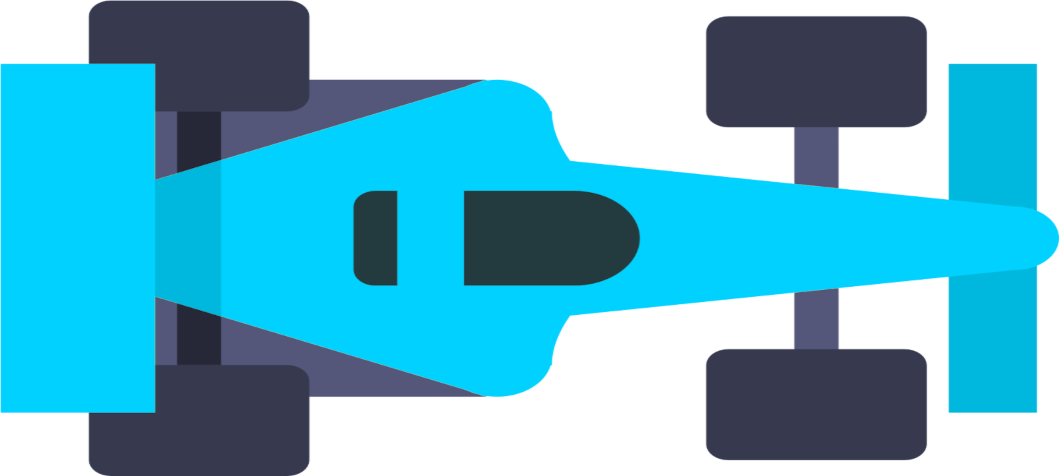
\includegraphics[width=0.3\linewidth]{images/car.png}
    \caption{Agente previo a la aplicación de la red neuronal}
    \label{fig:agente}
\end{figure}


\subsection{NEAT-Python}
El agente debe aprender a moverse en el entorno, NEAT permite que el agente recorra el espacio asignándoles valores de salida dependiendo de los valores de entrada. Los valores de entrada son valores que se toman del entorno, para este caso en particular, las entradas estarían dadas por el color de cada pixel, dependiendo del color del pixel, el agente cambia o no de dirección,  a esto se le conoce como acción o salida. NEAT le otorga al agente sensores que le permiten el reconocimiento del entrono, estos sensores son asignados para determinar cuando este sale de las vías, y la distancias entre puntos \cite{sensores}. En este articulo implementamos el uso de 5 sensores, asignados a una lista; -90°, -45,° 0°, 45° y 90°. Estas son las principales entradas para nuestro algoritmo NEAT aplicado al agente (Figura \ref{fig:agente}), ver Figura \ref{fig:agente_sensores}.

\begin{figure}
    \centering
    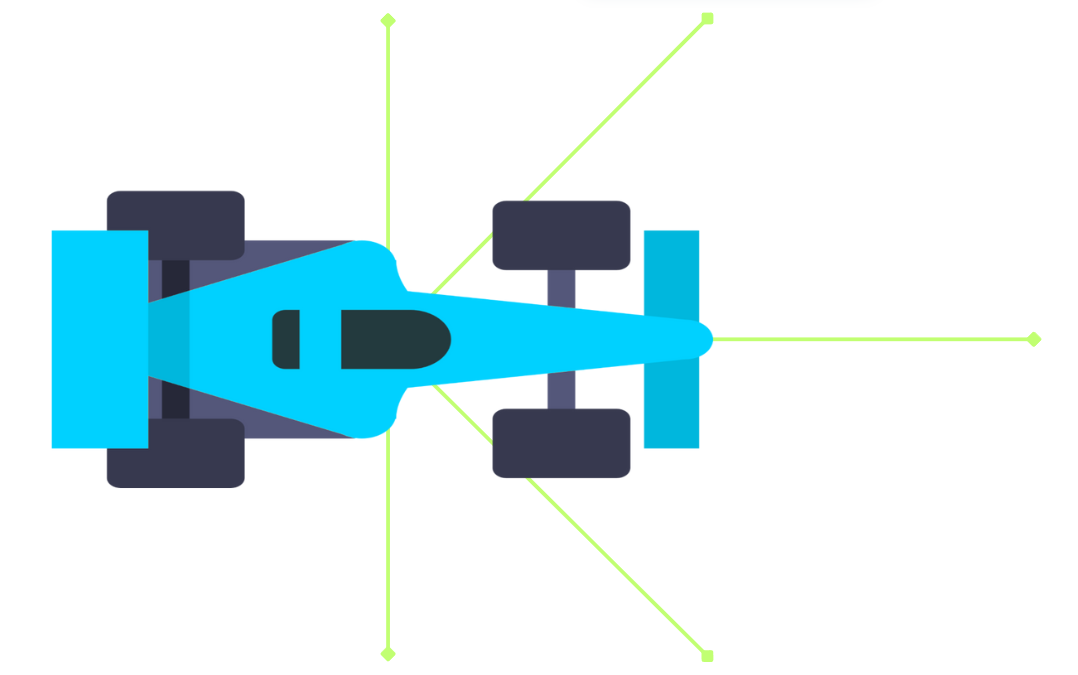
\includegraphics[width=0.5\linewidth]{images/sensores.png}
    \caption{Asignación de sensores al agente}
    \label{fig:agente_sensores}
\end{figure}



En la Figura \ref{fig:Red-neuronal},  Hidden o capas ocultas, son nodos que aplican un procesado a la entrada, con cada generación las capas aumentan dependiendo de la ganancia, esta ganancia está dada por las acciones previas del agente. Si el agente se desplaza en el mapa sin exceder las limitaciones, se mantiene en la generación. Las generaciones en NEAT es el umbral con el que se desea finalizar la simulación, por ejemplo, si se establecen 50 generaciones cada valor del umbral se le asocian a los agentes creados por la red neural aplicando distintos valores de configuración, si en la primera generación todos los carros chocan, se pasa a la siguiente generación, en este caso la segunda, así sucesivamente hasta llegar a la ultima que sería la generación 50. En el entrono se crean distintos agentes, cada agente recorre el mapa, si un agente choca o se sale de la vía, esta configuración tendrá menos probabilidad de replicarse, de esta manera se garantiza una generación final donde el o los agentes aprenda a desplazarse por el entorno de forma autónoma.

En la configuración inicial, Hidden es igual a 0, puesto que se inicia con una configuración sencilla, con cada generación Hidden aumenta para que la salida dada la entrada sea la mas óptima.

\begin{figure}
    \centering    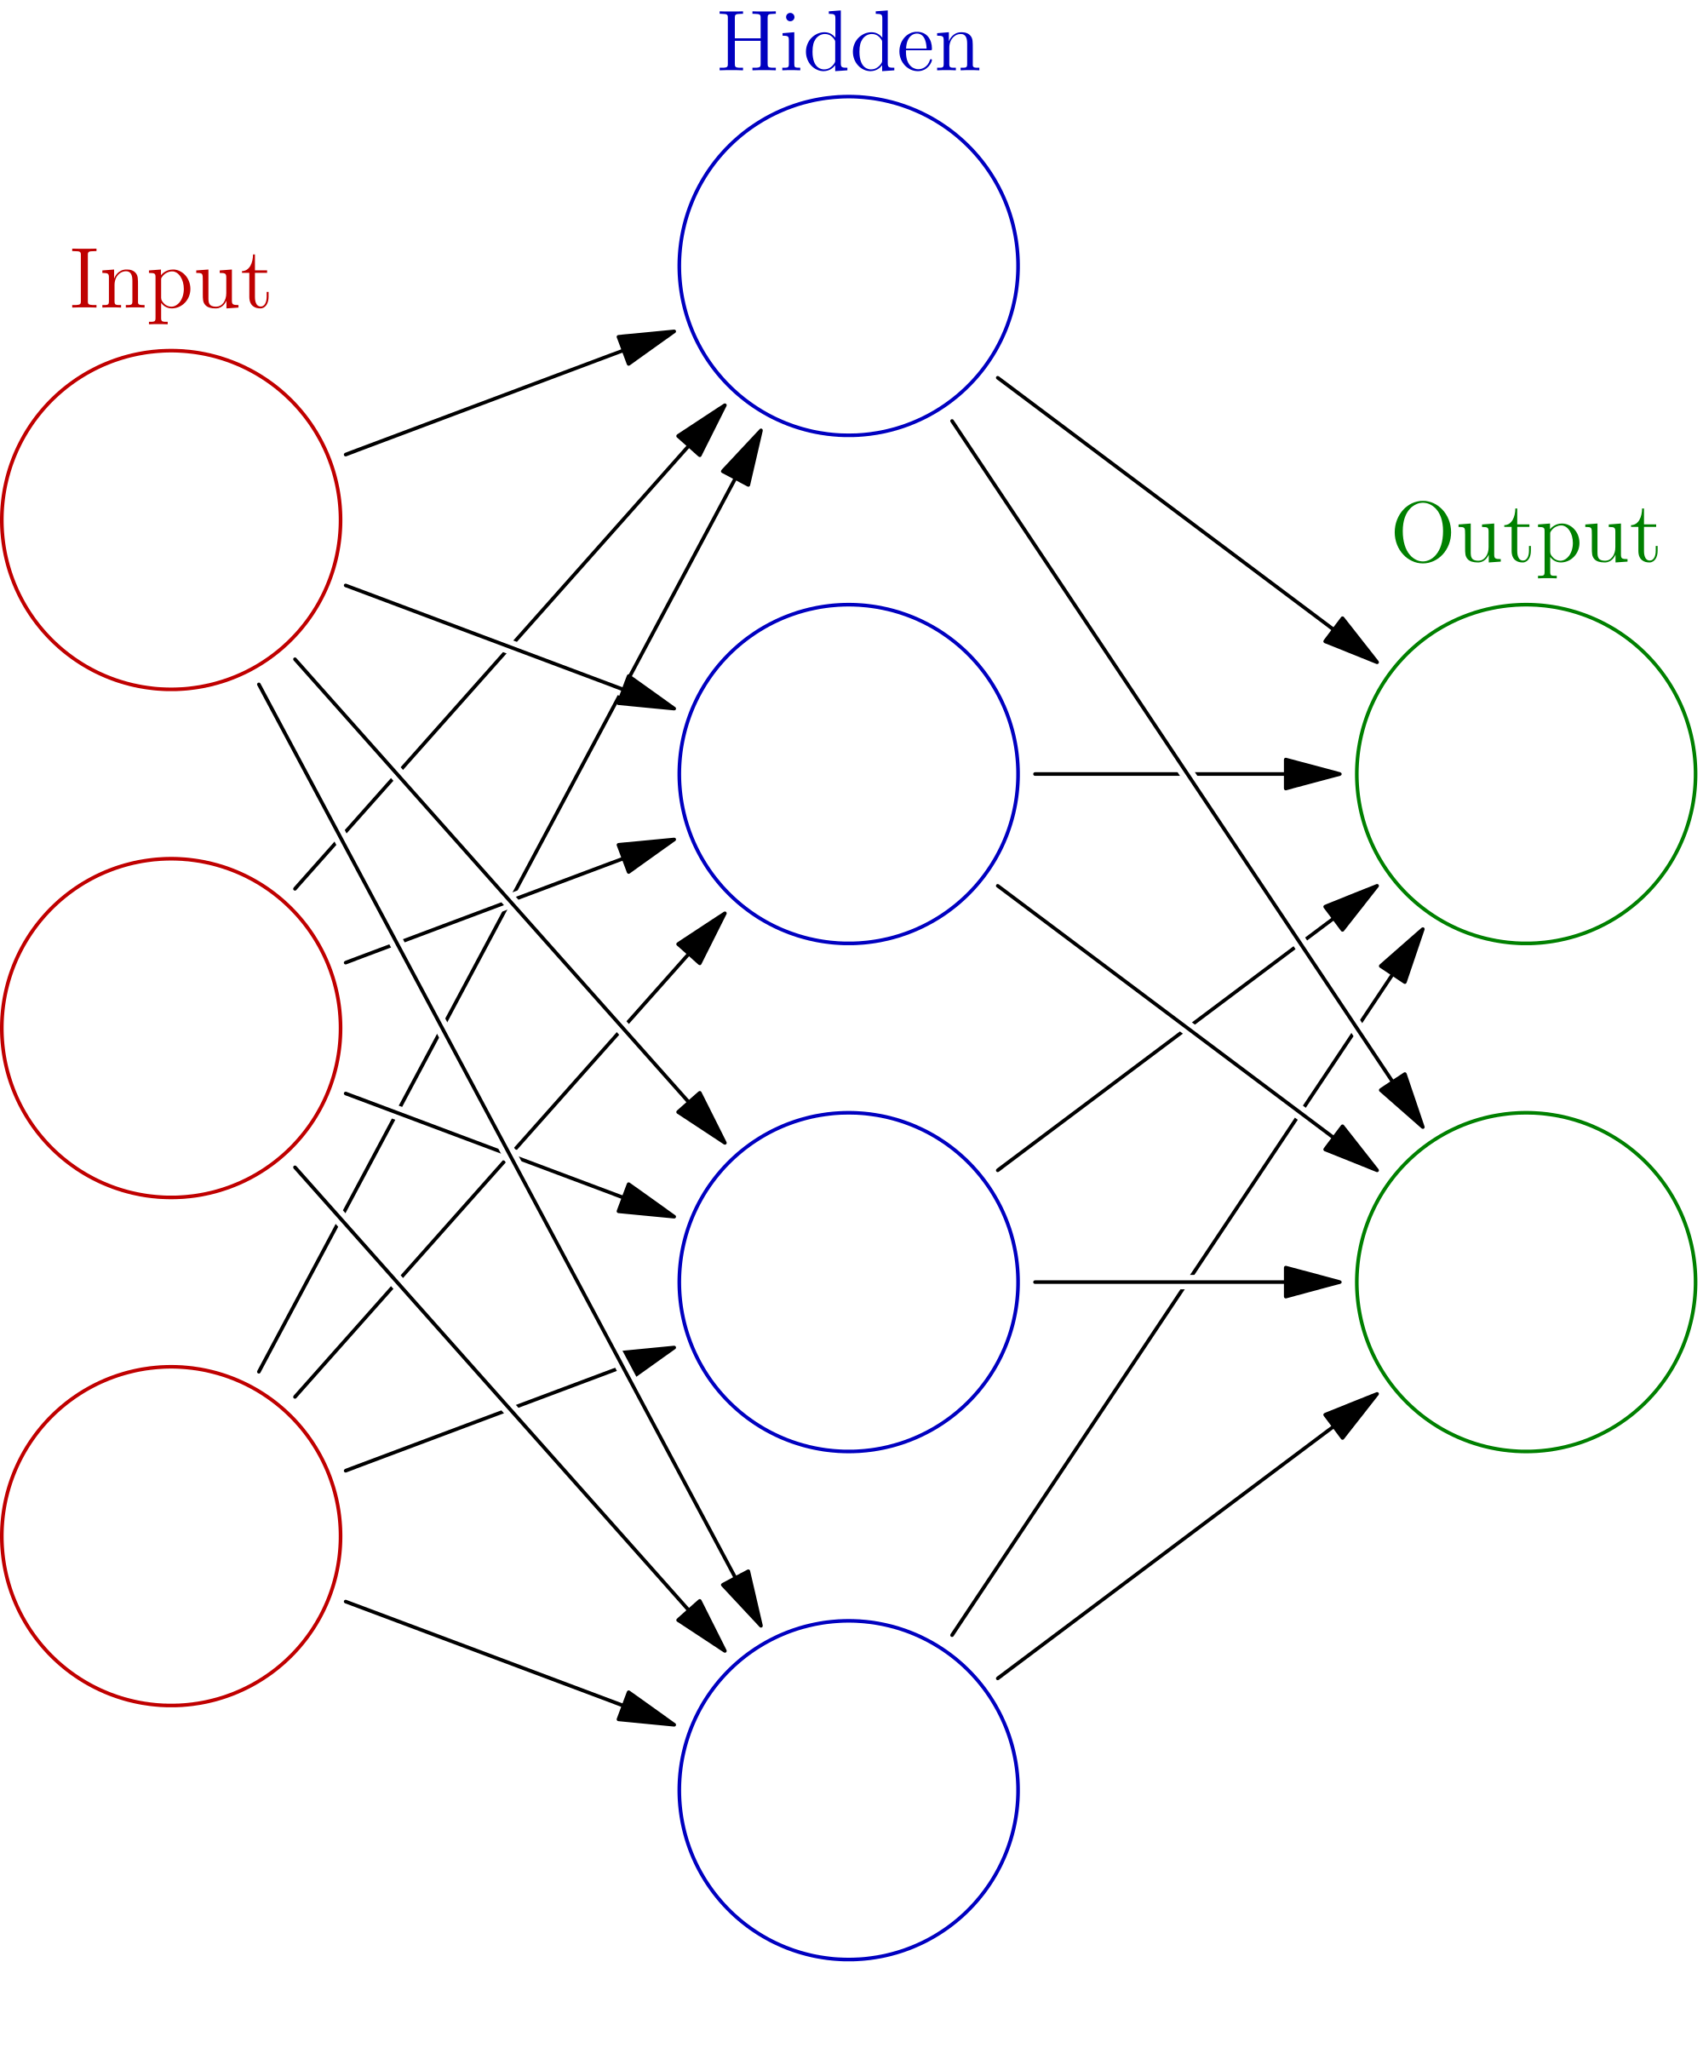
\includegraphics[width=0.5\linewidth]{images/neural_network.png}
    \caption{Estructura general de una red neuronal multicapa \cite{red_neuronal}}
    \label{fig:Red-neuronal}
\end{figure}

\subsection{Fitness function}
Para evaluar que tan bien son los genomas (próximas generaciones) NEAT implementa una función que evalúa que tan bien resuelve el problema en cuestión, esta función es llamada \textit{Fitness function}. Si un genoma A resuelve el problema de manera más exitosa que un genoma B, entonces el valor de aptitud de A debe ser mayor que el de B. La magnitud absoluta y los signos de estas aptitudes no son importantes, solo sus valores relativos, los pasos estarían dados por:
\begin{itemize}
    \item Crear una red neuronal: Basada en el genoma.
    \item Proveer entradas y calcular salidas: Por ejemplo, para cada caso en la tabla de verdad del XOR, se proporcionan las entradas a la red y se calcula la salida.
    \item Calcular el error: El error se calcula entre las salidas esperadas y las salidas reales de la red.
    \item Asignar aptitud: Si la red produce exactamente la salida esperada, su aptitud es 1. De lo contrario, es un valor menor a 1, disminuyendo más cuanto más incorrectas sean las respuestas de la red \cite{neat_python}.
\end{itemize}

La ecuación de actitud sería:
\begin{align*}
    Aptitud = 1 - \sum_{i} (e_i - a_i)^2,
\end{align*}
donde, $e_i$ (salidas esperadas): Son los valores que se esperan obtener de la red neuronal o agente autónomo. Las salidas esperadas son las posiciones ideales o los movimientos óptimos que el agente debería realizar para alcanzar el objetivo de la manera más eficiente posible. 

$a_i$ (salidas reales): Son los valores que realmente se obtienen de la red neuronal o agente autónomo. Estas son las posiciones o movimientos que el agente realiza durante su desplazamiento en el mapa.


%%%
\textit{Función de Aptitud}. En el contexto de nuestro proyecto, la función de aptitud es fundamental para evaluar y guiar el proceso de evolución de los agentes autónomos (vehículos) controlados por redes neuronales generadas mediante el algoritmo NEAT. 

Los pasos para calcular la aptitud de cada genoma son los siguientes:

\begin{itemize} 
\item \textbf{Crear una red neuronal}: Se genera una red neuronal basada en el genoma actual. 
\item \textbf{Simular el agente}: La red neuronal controla al agente autónomo en el entorno simulado (ver Figura \ref{fig:Mapa}), recibiendo entradas del entorno (como las distancias detectadas por los sensores del agente) y produciendo acciones (como cambios en la dirección y velocidad del agente). 
\item \textbf{Recopilar métricas}: Durante la simulación, se registran métricas relevantes, como la distancia mínima al objetivo, el tiempo de supervivencia y si el agente ha colisionado. 
\item \textbf{Calcular la aptitud}: Se utiliza una función de aptitud definida para calcular el valor de aptitud del genoma, basándose en las métricas recopiladas. 
La función de aptitud implementada es:
\begin{align*} 
    \text{Aptitud} = R_d
\end{align*}
donde $R_d$ es la recompensa por distancia al objetivo. 

\item \textbf{Recompensa por distancia al objetivo ($R_d$)}:

La recompensa por distancia es inversamente proporcional a la distancia $d_{agent}$ entre el agente y el objetivo:

\begin{align*} 
R_d = \begin{cases} 
10000, \quad \text{si } \quad d_{agent} = 0 
\cr 10000-d_{agent}, \quad \text{si} \quad d_{agent} > 0 
\end{cases} 
\end{align*}

Donde para la distancia Euclidiana $d_{agent}$ se calcula como:
\begin{align*} 
    d_{agent} = {\sqrt{(x_{agent} - x_{goal})^2 + (y_{agent} - y_{goal})^2}} 
\end{align*}

Para la distancia de Manhattan $d_{agent}$ se calcula como:
\begin{align*} 
    d_{agent} = |x_{agent} - x_{goal}| + |y_{agent} - y_{goal}|
\end{align*}

El tercer y último método es la distancia de Chebyshev, esta es calculada de la siguiente manera 
\begin{align*} 
    d_{agent} = \max(|x_{agent} - x_{goal}|, |y_{agent} - y_{goal}|)
\end{align*}



Aquí, $(x_{\text{agent}}, y_{\text{agent}})$ son las coordenadas actuales del agente, y $(x_{\text{goal}}, y_{\text{goal}})$ son las coordenadas de cada punto objetivo en la lista de objetivos. Esta recompensa incentiva al agente a acercarse lo más posible al objetivo.\\
\end{itemize}

Combinando los términos anteriores, la función de aptitud se expresa como:
\begin{align*} 
Aptitud = 10000 - d_{agent} 
\end{align*}
Además, para asegurar que el valor de aptitud no sea negativo, se aplica:
\begin{align*} 
Aptitud = \max(0, Aptitud) 
\end{align*}

Entre mayor sea la aptitud, los genomas con sus características aumentan las probabilidades de ser seleccionados para la próxima generación.
%%%
\begin{figure}
    \centering
    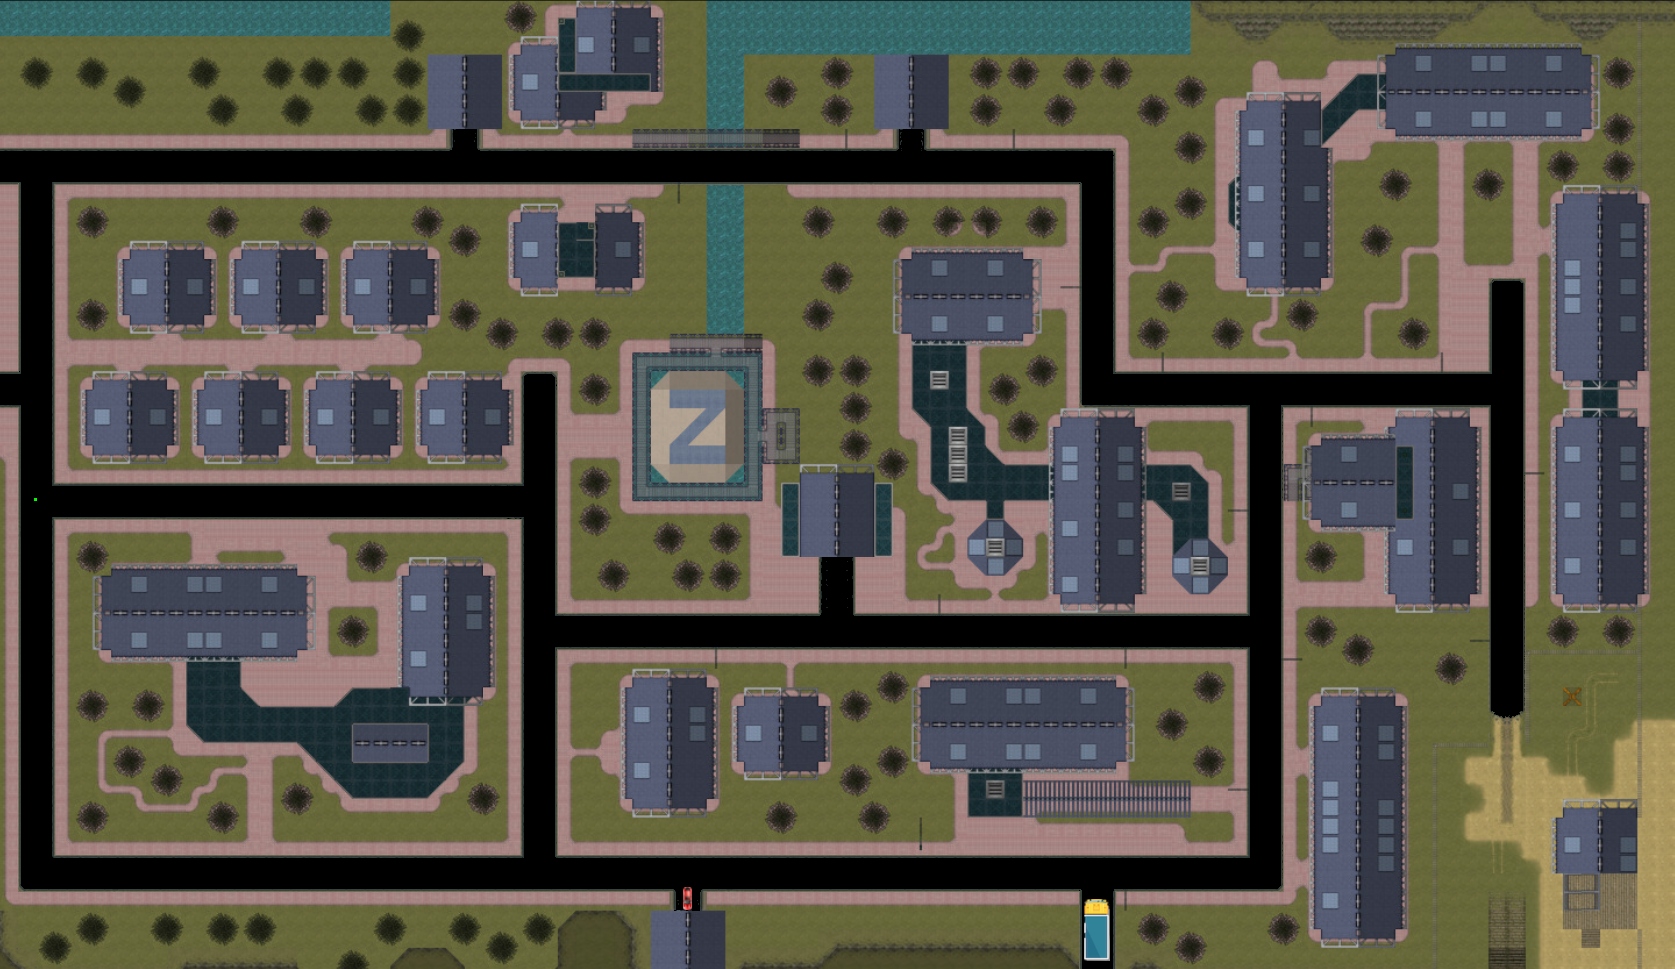
\includegraphics[scale=0.14]{images/gta2.png}
    \caption{Mapa del entorno donde el agente autónomo realizará su aprendizaje}
    \label{fig:Mapa}
\end{figure} 

\subsection{Implementación de asignación entrada  salida}
Dadas las entradas de los sensores, se le asigna un angulo de rotación y una velocidad al agente autónomo, es un esquema básico, pero funcional ver Figura \ref{fig:Bucle_basico}. Sin embargo, que pasa si las variaciones de los ángulos son muy altas, o tal vez muy bajas, o quizá la velocidad es muy lenta?
\begin{figure}
    \centering
    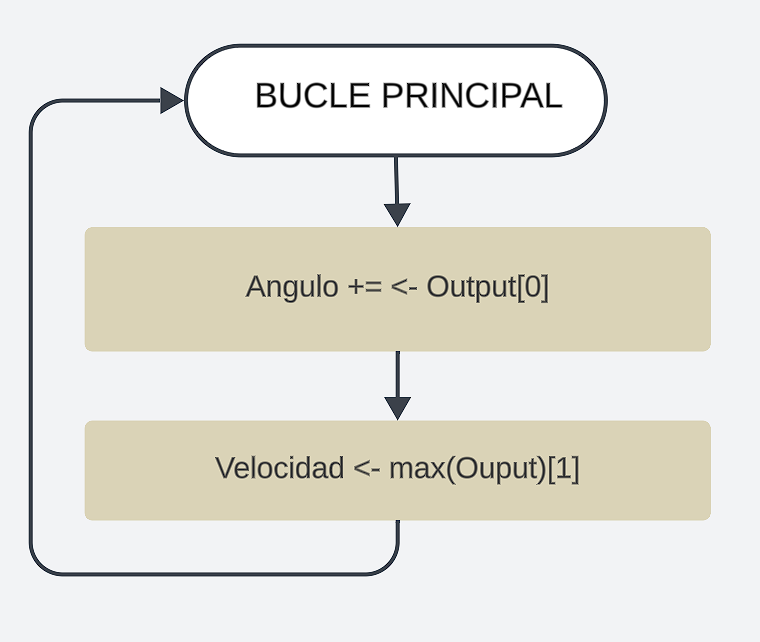
\includegraphics[scale=0.25]{images/bucle_inicial.png}
    \caption{Bucle básico de como el agente autónomo es retroalimentado con las entradas}
    \label{fig:Bucle_basico}
\end{figure} 
Las altas variaciones de los ángulos genera inconvenientes, uno de ellos es causar que el agente gire sin parar. Si el agente recibe una entrada constante de ángulos en una misma dirección, ocasiona que la suma constante de esos ángulos lo haga girar, más si dichas entradas se presentan en las primeras generaciones. Por contraparte, su desplazamiento se ve disminuido, lo que implica un estancamiento del agente. En el caso de que la entrada sea demasiada alterada pero iterando la dirección de los ángulos, su velocidad también es reducida, ya que si no lo hace, el carro será eliminado debido al inminente hecho de chocar con los bordes fuera de la zona establecida como carretera.

Para evitar alguna de las singularidades (asúmase singularidad como estancamiento, rotación sin parar) se asigna un \textbf{Set\_Valor} a la velocidad si la velocidad previa del agente es menor a 0.1, esto evita que el agente avance demasiado lento, optimizando en medida el tiempo de cada simulación, en este articulo, \textbf{Set\_Valor} es igual a 5. A esta asignación la denominamos \textit{Refuerzo forzado} o \textit{Método de aceleración}, y su diagrama es presentado en la Figura \ref{fig:reforce}.

\begin{figure}
    \centering
    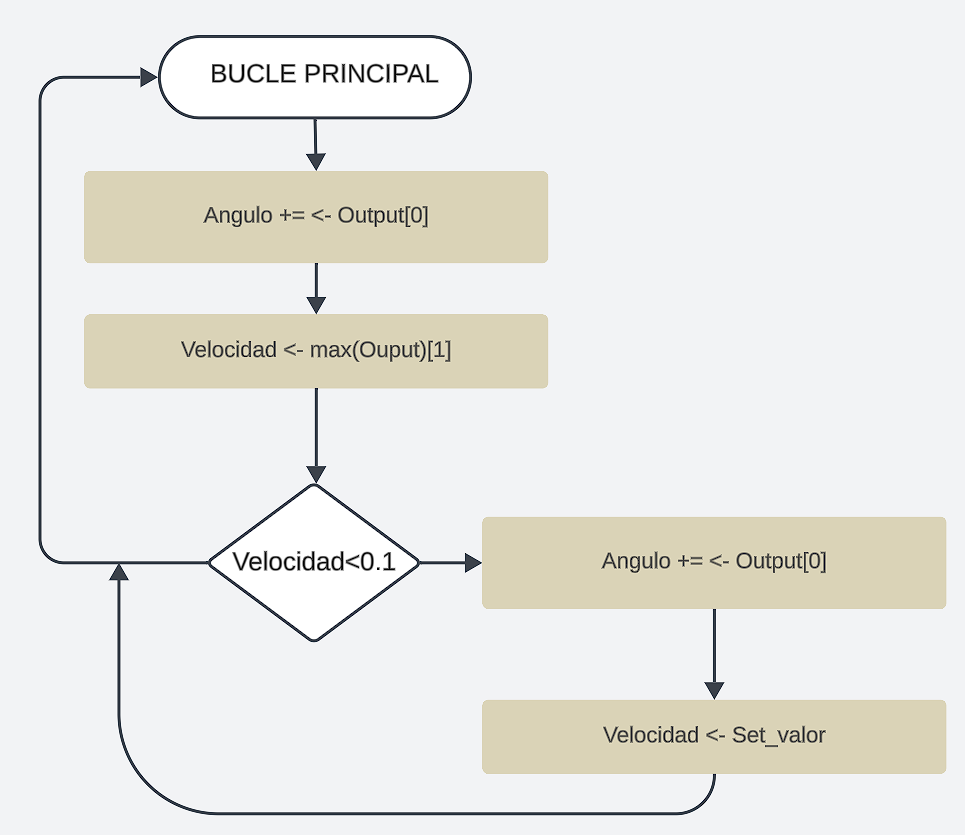
\includegraphics[width=0.7\linewidth]{images/reforce.png}
    \caption{Diagrama de flujo de la función de aceleración o refuerzo forzado, diseñada para optimizar y reducir el estancamiento de algunos agentes en primeras generaciones.}
    \label{fig:reforce}
\end{figure}

Una vez establecidos los parámetros iniciales, se realizan distintas simulaciones con el fin de recopilar datos para analizar el comportamiento de los agentes. Se realizaron un total de 48 simulaciones para el primer mapa (Figura \ref{fig:Mapa}), distribuidas en grupos de tres, 20 simulaciones para la distancia Manhattan, 20 para la Euclidiana y 20 para la distancia Chebyshev. Se distribuyen de como se muestra en la Tabla \ref{tab:fds}. A cada número de generación le corresponden 5 simulaciones, es decir en la distancia Euclidiada según la tabla fue un total de $3*5 = 15$ simulaciones realizadas, donde 5 fueron las simulaciones realizadas con una generación de 20, otras 5 para la generación de 30 y por último otras 5 para la generación de 50; así para la distancia Manhattan y Chebyshev. Estas fueron realizadas con la aplicación del método \textbf{Refuerzo forzado} (ver Figura \ref{fig:reforce}), además se realizaron tres simulaciones adicionales sin este método. Corresponden a una simulación de 50 generaciones para las tres distancias aplicadas, por ende el total de simulaciones son las 45 contadas anteriormente, más 3 simulaciones sin la aplicación de este método, como se observa en la Tabla \ref{tab:fds_1}.

\begin{table}
\centering
\caption{Configuración de simulaciones del agente en el entorno por cada métrica}
\label{tab:fds}
\begin{tabular}{ll}
\toprule
\textbf{Simulaciones} & \textbf{Generaciones} \\
\midrule
Euclidiana (5)   &  20, 30, 50 \\
Manhattan (5)    & 30, 30, 50 \\
Chebyshev (5)    & 20, 30, 50 \\
\bottomrule
\end{tabular}
\end{table}


\begin{table}
\centering
\caption{Orden de simulaciones}
\label{tab:fds_1}
\begin{tabular}{lll}
\toprule
\textbf{Simulaciones} & 
\textbf{Generaciones}  &
\textbf{Refuerzo forzado}\\
\midrule
Euclidiana (5)   &  20, 30, 50 & SI\\
Manhattan (5)     &  20, 30, 50 & SI\\
Chebyshev (5)     &  20, 30, 50 & SI\\
\bottomrule
Euclidiana (1)    & 50 & NO\\
Manhattan (1)     & 50 & NO\\
Chebyshev  (1)    & 50 & NO\\
\bottomrule
\end{tabular}
\end{table}

También se realizaron 15 simulaciones adicionales para un segundo mapa ver Figura \ref{fig:mapa2}, en estas simulaciones solo se realizaron para una generación de 50, como se indica en la Tabla \ref{tab:fds_2},donde (5) representan las simulaciones realizadas, siguiendo el orden planteado anteriormente, 5 simulaciones realizadas para la distancia Euclidiana con una generación de 50, y así para la distancia Manhattan y Chebyshev, para un total de $5*3=15$ simulaciones.

\begin{table}
\centering
\caption{Orden de simulaciones}
\label{tab:fds_2}
\begin{tabular}{lll}
\toprule
\textbf{Simulaciones} & 
\textbf{Generaciones}  &
\textbf{Refuerzo forzado}\\
\midrule
Euclidiana (5)   &50 & SI\\
Manhattan (5)     &50 & SI\\
Chebyshev (5)     &50 & SI\\
\bottomrule
\end{tabular}
\end{table}


\begin{figure}
    \centering    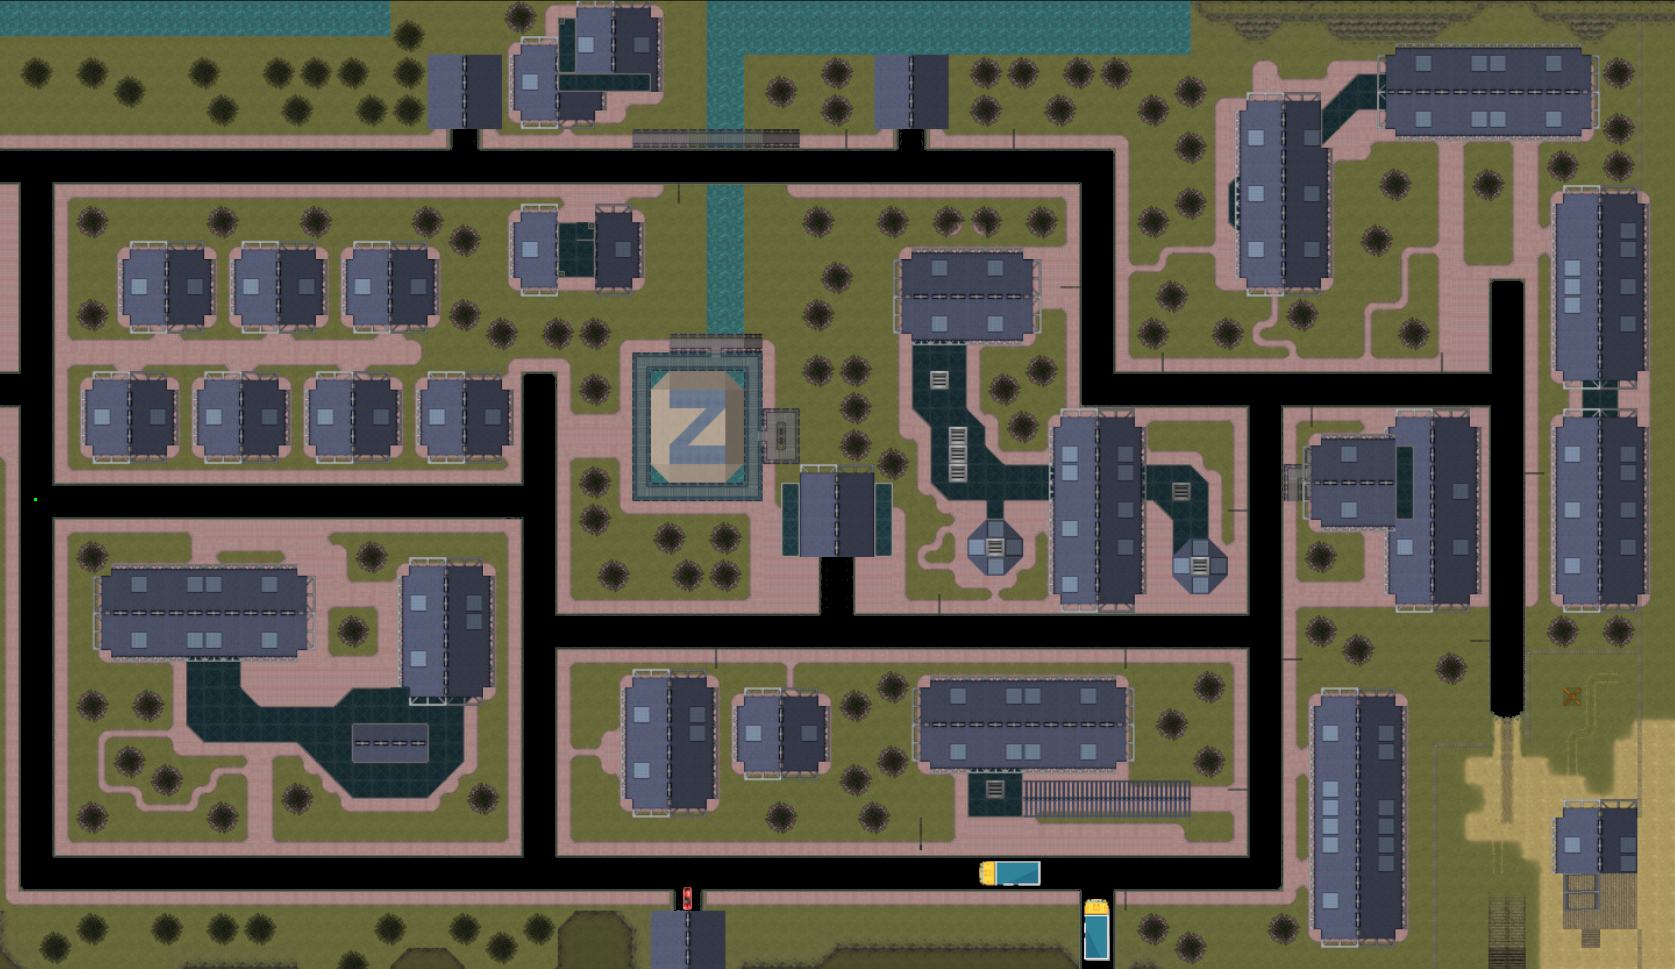
\includegraphics[width=0.8\linewidth]{Simulacion/gta.png}
    \caption{Mapa con bloqueo de vía inferior}
    \label{fig:mapa2}
\end{figure}

\section{Resultados}
Los registros obtenidos de las simulaciones contienen el fitness promedio de los genomas, el mejor fitness de la simulación, por últimos las máximas y mínimas recompensas. Con estos datos, se obtiene la gráfica el fitness promedio con las desviaciones presentadas.

\subsection{Configuración del mapa implementado en la simulación}
Durante la preparación del mapa para la simulación, a los bordes principales de la carretera se les asigno un color RGB(20, 23.5, 21.6) (ver Figura \ref{fig:Bordes}.) Sin embargo, en la configuración para determinar los limites de la vía se opta por establecer que los limites son todos los colores distintos del negro.
\begin{figure}[ht]
    \centering    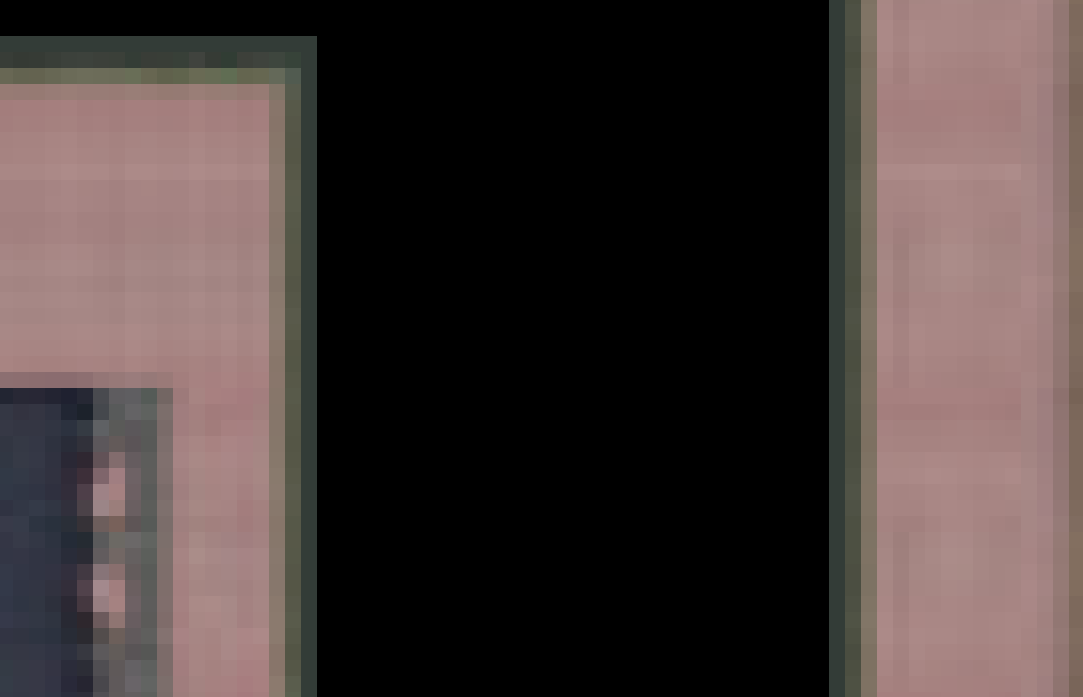
\includegraphics[width=0.4\linewidth]{Simulacion/Bordes.png}
    \caption{Bordes laterales de la vía usada en el mapa}
    \label{fig:Bordes}
\end{figure}


\subsection{Configuraciones principales del algoritmo NEAT}
El archivo de configuración para NEAT consta de distintas secciones, cada una de ellas orientada a como será la creación de generaciones en cada simulación. En la sección [NEAT] \ref{tab:NEAT}, se pueden encontrar los parámetros fitness y el tamaño de la población en cada generación; en la sección [DefaultReproduction] \ref{tab:DefaultReproduction}, podemos encontrar la configuración de elitism y survival threshold, que permiten determinar el numero de especies mas aptas de cada generación que se desea conservar, y la proporción de cada especie permitida para reproducirse en cada generación; en la sección [DefaultGenome] \ref{tab:DefaultGenome}, se define los parámetros específicos para la estructura de los genemoas (redes neuronales) que Neat evolucionará, como el modo de activación o activation defauld y activation mutate rate.
\begin{table}
    \centering
    % Primera tabla
    \captionof{table}{\texttt{[NEAT]}}
    \label{tab:NEAT}
    \begin{tabular}{ll}
    \toprule
    \textbf{Variable} & \textbf{Valor} \\
    \midrule
    fitness\_criterion     & max \\
    fitness\_threshold     & 10000 \\
    pop\_size              & 50 \\
    reset\_on\_extinction  & True  \\
    \bottomrule
    \end{tabular}
    \vspace{0.5cm}
    
    % Segunda tabla
    \captionof{table}{\texttt{[DefaultReproduction]}}
    \label{tab:DefaultReproduction}
    \begin{tabular}{ll}
    \toprule
    \textbf{Variable} & \textbf{Valor} \\
    \midrule
    excess\_coeff            & 1.0 \\
    disjoint\_coeff          & 1.0 \\
    weight\_diff\_coeff      & 0.5 \\
    compatibility\_threshold & 3.0 \\
    elitism                  & 5 \\
    survival\_threshold      & 0.2 \\
    \bottomrule
    \end{tabular}
    \vspace{0.5cm}
\end{table}

\begin{table}
    % Tercera tabla
    \centering
    \captionof{table}{\texttt{[DefaultGenome]}}
    \label{tab:DefaultGenome}
    \begin{tabular}{ll}
    \toprule
    \textbf{Variable} & \textbf{Valor} \\
    \midrule
    \multicolumn{2}{l}{\textbf{Opciones de Activación de Nodos}} \\
    activation\_default       & tanh \\
    activation\_mutate\_rate  & 0.01 \\
    activation\_options       & tanh, relu, sigmoid \\
    \addlinespace
    
    \multicolumn{2}{l}{\textbf{Opciones de Agregación de Nodos}} \\
    aggregation\_default      & sum \\
    aggregation\_mutate\_rate & 0.01 \\
    aggregation\_options      & sum \\
    \addlinespace
    
    \multicolumn{2}{l}{\textbf{Opciones de Sesgo de Nodos}} \\
    bias\_init\_mean         & 0.0 \\
    bias\_init\_stdev        & 1.0 \\
    bias\_max\_value         & 30.0 \\
    bias\_min\_value         & -30.0 \\
    bias\_mutate\_power      & 0.5 \\
    bias\_mutate\_rate       & 0.7 \\
    bias\_replace\_rate      & 0.1 \\
    \addlinespace
    
    \multicolumn{2}{l}{\textbf{Opciones de Compatibilidad del Genoma}} \\
    compatibility\_disjoint\_coefficient & 1.0 \\
    compatibility\_weight\_coefficient   & 0.5 \\
    \addlinespace
    
    \multicolumn{2}{l}{\textbf{Tasas de Adición/Eliminación de Conexiones}} \\
    conn\_add\_prob        & 0.5 \\
    conn\_delete\_prob     & 0.5 \\
    \addlinespace
    
    \multicolumn{2}{l}{\textbf{Opciones de Habilitación de Conexiones}} \\
    enabled\_default       & True \\
    enabled\_mutate\_rate  & 0.1 \\
    \addlinespace
    
    \multicolumn{2}{l}{\textbf{Configuraciones de Topología}} \\
    feed\_forward          & False \\
    initial\_connection    & full \\
    \addlinespace
    
    \multicolumn{2}{l}{\textbf{Tasas de Adición/Eliminación de Nodos}} \\
    node\_add\_prob        & 0.2 \\
    node\_delete\_prob     & 0.2 \\
    \bottomrule
    \end{tabular}
\end{table}

\subsection{Resultados de las simulaciones aplicando la distancia Euclidiana}
\textbf{50 Generaciones}\\
Durante las simulaciones realizadas se almacenaron los datos del fitness correspondiente a esta distancia, las primeras 5 simulaciones realizadas correspondieron a la generación número 50, como resultado se obtuvo la Figura \ref{fig:Euclidiana_50_refuerzo}. La zona sombreada corresponde a las desviaciones de cada simulación, estas desviaciones indican agentes alejados del promedio, basándose en ello se puede observar que simulaciones obtuvieron la mayor cantidad de puntos.

\begin{figure}[H]
    \centering    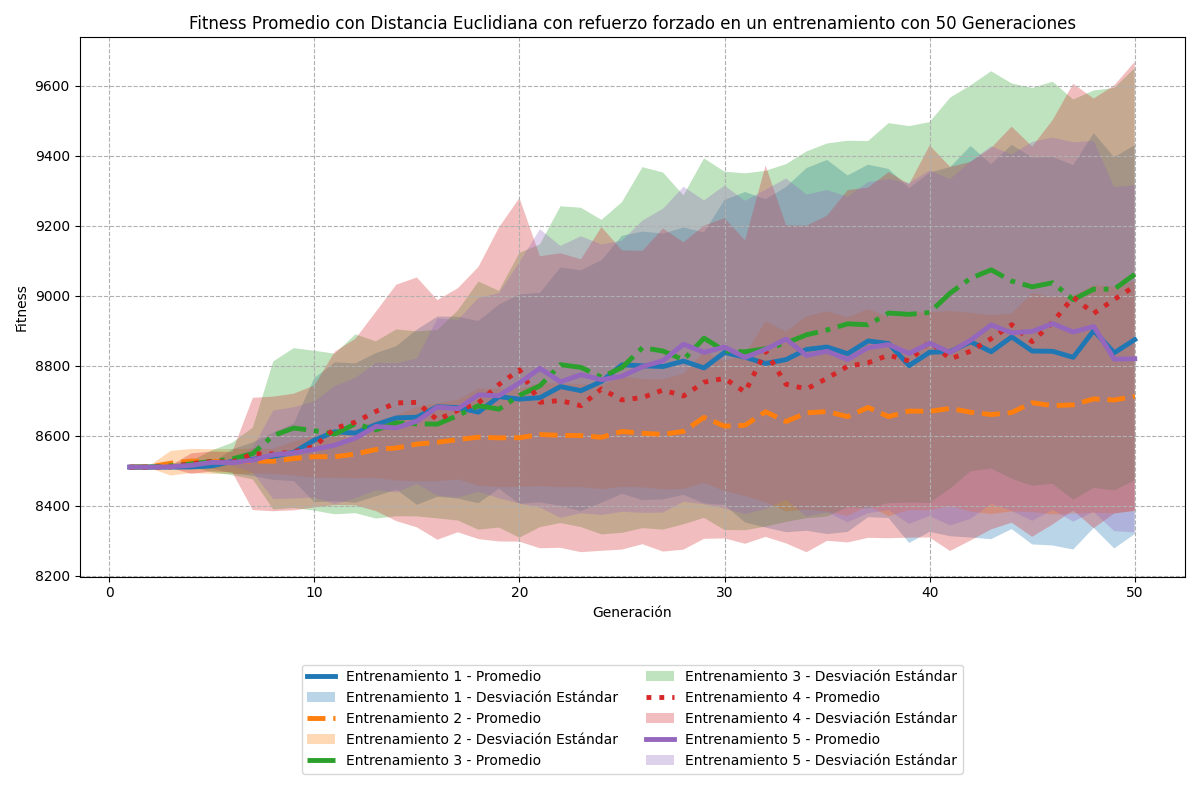
\includegraphics[width=0.9 \linewidth]{Euclidiana/Fitness_Acumulado_Eucli_50Gen.png}
    \caption{Gráfica de promedios y desviaciones fitness correspondiente a 5 simulaciones realizadas con una generación de 50}
    \label{fig:Euclidiana_50_refuerzo}
\end{figure}

De manera individual, el entrenamiento 4 obtuvo el fitness máximo, con un valor exacto de 9990, como se aprecia en la Figura \ref{fig:Fitnes_ecu_4_50_inv}. Ademas, este entrenamiento presentó la mayor desviación, como se observa en la Figura \ref{fig:Fitnes_ecu_4_50_inv_sombra}.\\

%El segundo fitness más alto le corresponde al entrenamiento 1, con un valor de 9988, además otra característica para el primer entrenamiento corresponde a la desviación, esta sobrepasa los 9400, sin embargo respecto al cuarto entrenamiento su desviación son 200 puntos por debajo (Fig. \ref{fig:eucli_1_50} y \ref{fig:eucli_1_50_sombra}). Seguido de este entrenamiento, el tercer entrenamiento obtuvo un fitness de 9985, con una desviación de 9600, misma desviación que el cuarto entrenamiento (Fig. \ref{fig:eucli_3_50} y \ref{fig:eucli_3_50_sombra}). El quinto entrenamiento obtuvo un fitness de 9982, con una desviación de 9400, en el mismo rango de desviación que el primer entrenamiento (Fig. \ref{fig:eucli_5_50} y \ref{fig:eucli_5_50_sombra}). Para finalizar, el entrenamiento 2 obtuvo el fitnes más bajo con un puntaje de 9626, con la menor desviación de las 5 simulaciones (Fig. \ref{fig:eucli_2_50} y \ref{fig:eucli_2_50_sombra}).

%%%%%%%%%%%%%%%%

\textbf{30 Generaciones}\\
Con los datos recopilados en estas 5 simulaciones para esta generación, la gráfica obtenida se observa en la Figura \ref{fig:Euclidiana_30_refuerzo}. Los entrenamientos que presentan las mayores desviaciones fueron el primer, tercer y quinto entrenamiento. El fitness máximo corresponde al tercer entrenamiento con 9986 como se aprecia en la Figura \ref{fig:Fitnes_ecu_3_30_inv}, ademas presentó la mayor desviación de todas para esta sección, con un valor de 9400 (ver Figura \ref{fig:Fitnes_ecu_3_30_inv_sombra}).
\begin{figure}[H]
    \centering    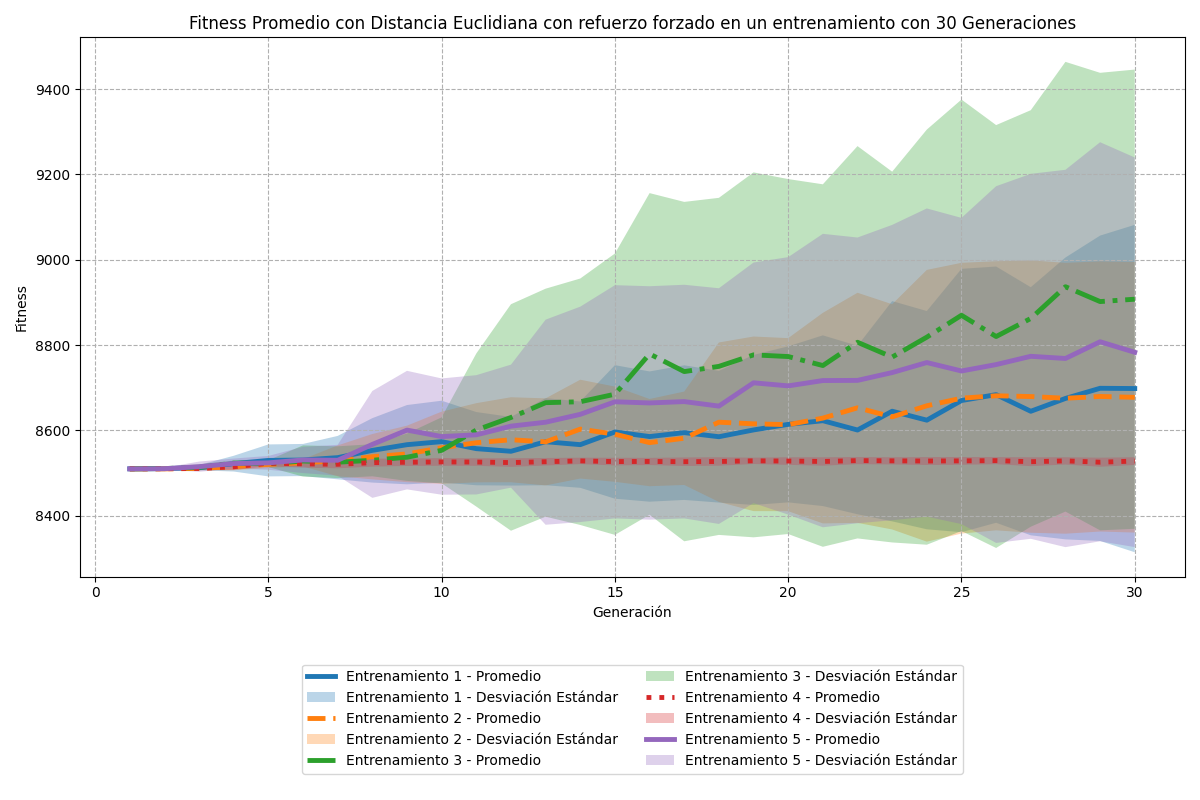
\includegraphics[width=0.99 \linewidth]{Euclidiana/Fitness_Acumulado_Eucli_30Gen.png}
    \caption{Gráfica de promedios y desviaciones fitness correspondiente a 5 simulaciones realizadas con una generación de 30}
    \label{fig:Euclidiana_30_refuerzo}
\end{figure}


El segundo fitness mas alto le corresponde al entrenamiento 5, con un valor de 9984, seguido de este entrenamiento, el primer entrenamiento obtuvo un fitness de 9981, con una desviación que se aproxima a los 9100, 100 puntos menos que la desviación correspondiente al quinto entrenamiento (Fig. \ref{fig:eucli_5_30}, \ref{fig:eucli_5_30_sombra}, \ref{fig:eucli_1_30} y  \ref{fig:eucli_1_30_sombra}). Para el segundo entrenamiento la diferencia con respecto al primero es de 98 puntos por debajo, con un fitness máximo de 9883, y una desviación de 9000 (Fig. \ref{fig:eucli_2_30} y \ref{fig:eucli_2_30_sombra}). Por último, el cuarto entrenamiento obtuvo el fitness mas bajo con 8544, con una desviación que no supera los 8600 (Fig. \ref{fig:eucli_4_30} y \ref{fig:eucli_4_30_sombra}).

\subsubsection{20 Generaciones}
La gráfica general de las desviaciones y promedios obtenidos en estas simulaciones es:
\begin{figure}[H]
    \centering    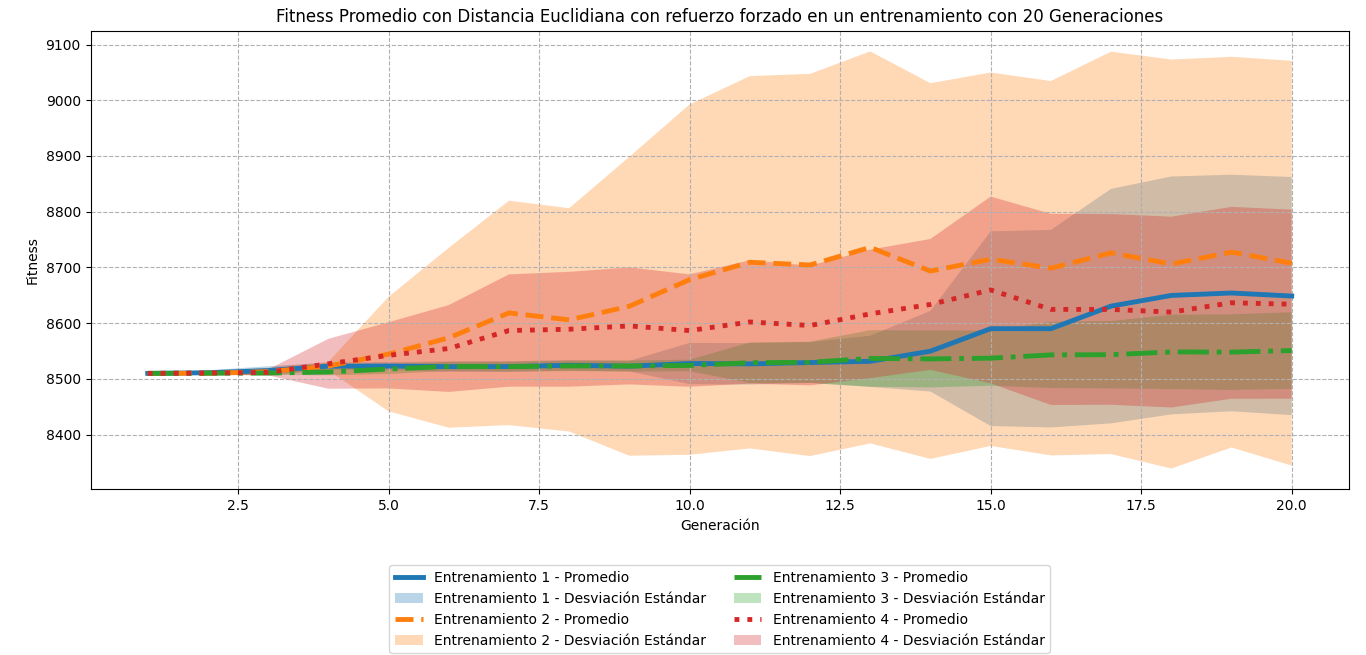
\includegraphics[width=0.99 \linewidth]{Euclidiana/Fitness_Acumulado_Eucli_20Gen.png}
    \caption{Gráfica de promedios y desviaciones fitness correspondiente a 5 simulaciones realizadas con una generación de 20}
    \label{fig:Euclidiana_20_refuerzo}
\end{figure}
Como se puede observar, la desviación con mayor valor se obtuvo en el segundo entrenamiento, además su puntaje fitness fue el mas alto de todos los demás con un valor de 9881:
\begin{figure}[H]
    \centering
    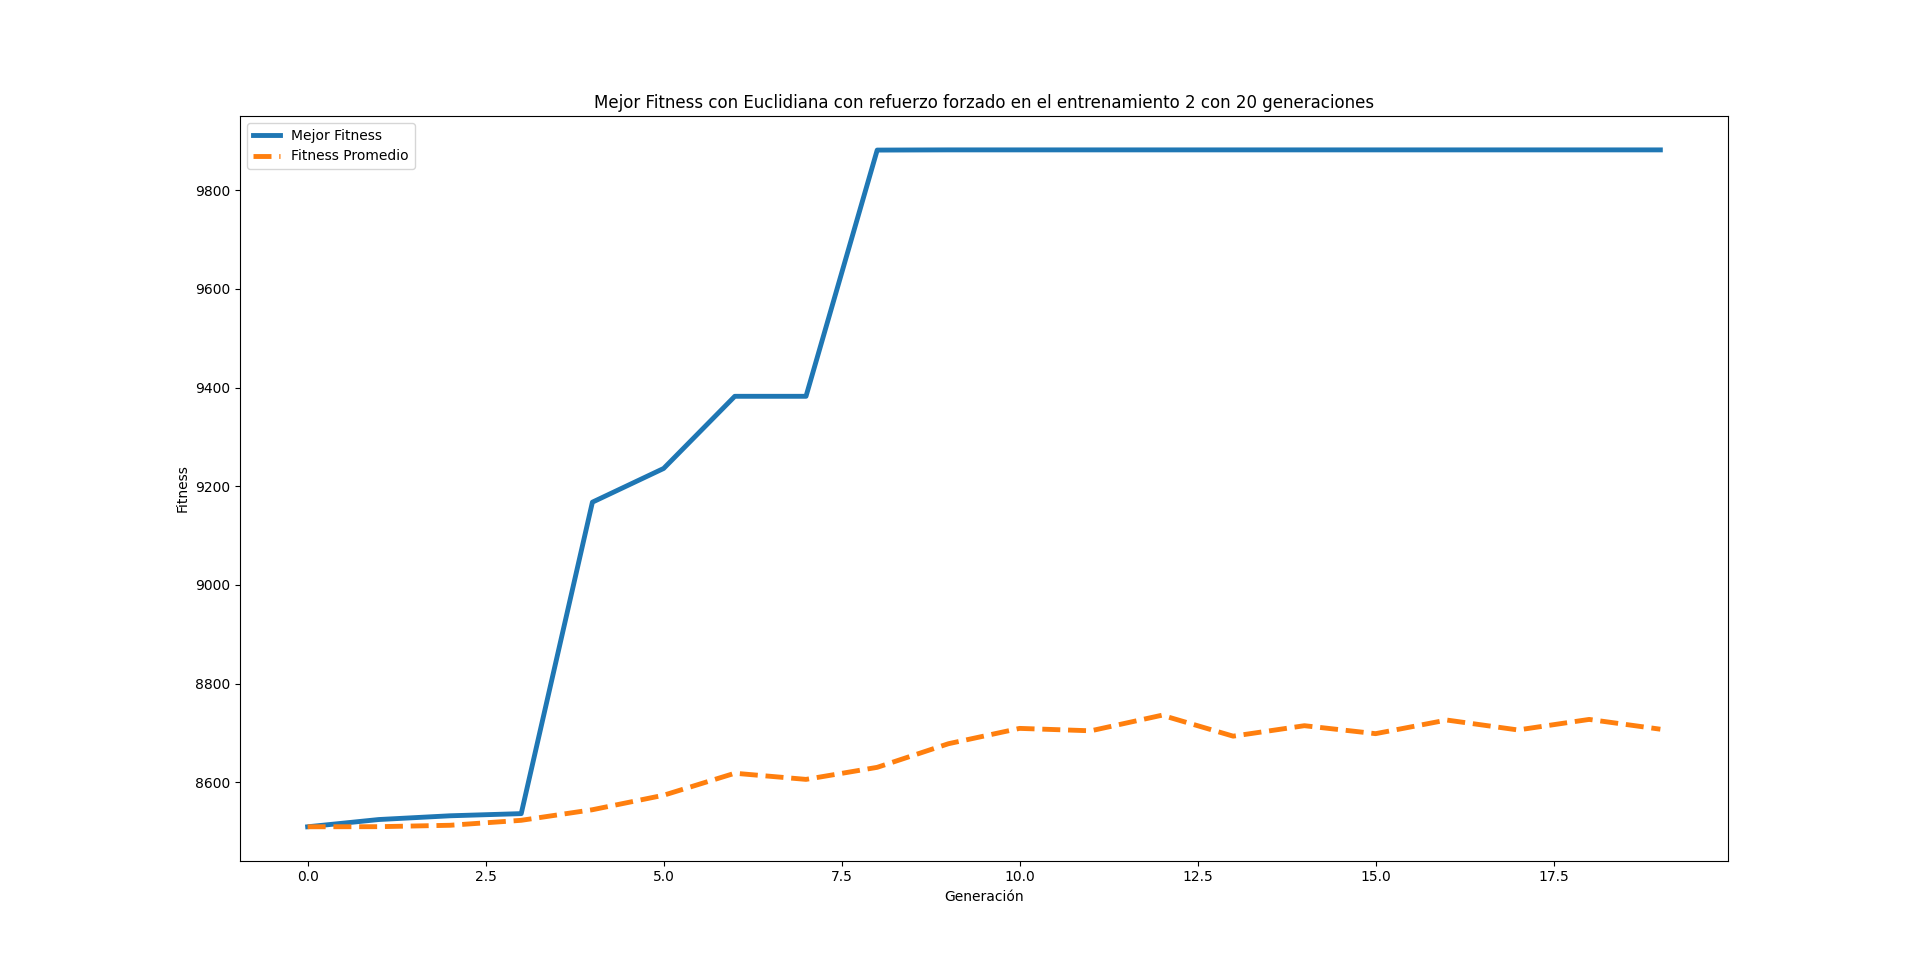
\includegraphics[width=0.9\linewidth]{Euclidiana/Fitness_individual_20/Fitness_2_Eucli_20Gen.png}
    \caption{Fitness individual para el entrenamiento 2 de 20 generaciones aplicando la distancia Euclidiana}
    \label{fig:Fitnes_ecu_2_20_inv}
\end{figure}
La gráfica de desviación es:
\begin{figure}[H]
    \centering
    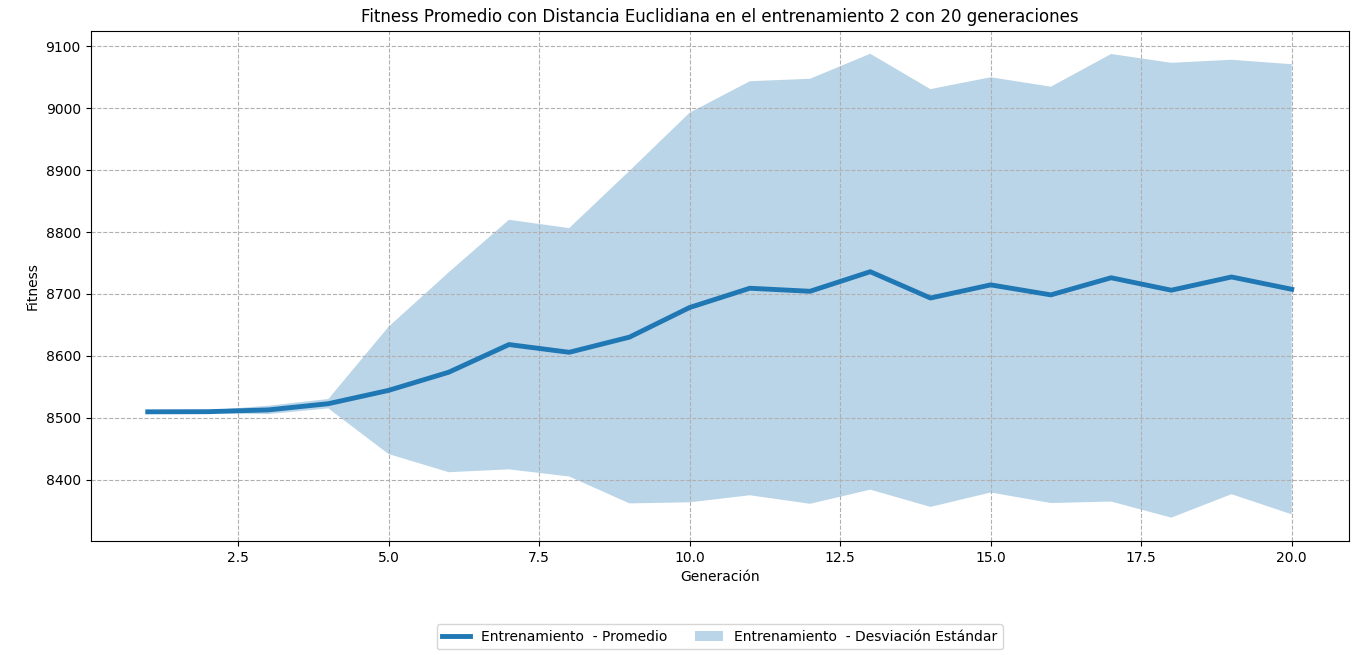
\includegraphics[width=1\linewidth]{Euclidiana/Fitness_individual_20/Fitness_2_Eucli_20Gen_Sombra.png}
    \caption{Fitness promedio y desviación individual para el entrenamiento 2 de 20 generaciones aplicando la distancia Euclidiana}
    \label{fig:Fitnes_ecu_2_20_inv_sombra}
\end{figure}
Con un fitness maximo de 9632, el primer entrenamiento obtuvo el segundo mejor puntaje, con una desviación por encima de los 8800; para el cuarto entrenamiento el puntaje máximo fue de 9237,también sobrepasando los 8800, sin emabrgo el fitness promedio durante la genración 17 y 20 fue en un rango de 8600 y 8650 puntos (Fig. \ref{fig:eucli_1_20}, \ref{fig:eucli_1_20_sombra}, \ref{fig:eucli_4_20} y \ref{fig:eucli_4_20_sombra}). Por último, el quinto y tercer entrenamiento obtuvieron los fitness mas bajos con 8782 y 8773, con una desviación que no supera los 8750 (Fig. \ref{fig:eucli_5_20}, \ref{fig:eucli_5_20_sombra}, \ref{fig:eucli_3_20} y \ref{fig:eucli_3_20_sombra}).



\subsection{Resultados de las simulaciones aplicando la distancia Manhattan}
\subsubsection{50 Generaciones}
Principalmente se iniciaron las simulaciones para las 50 generaciones, de estas simulaciones se graficaron los mejores promedios y las desviaciones de cada entrenamiento, de esta manera la grafica que reúne cada uno de los entrenamientos es la Figura \ref{fig:Manhattan_50_genral}.
\begin{figure}[H]
    \centering
    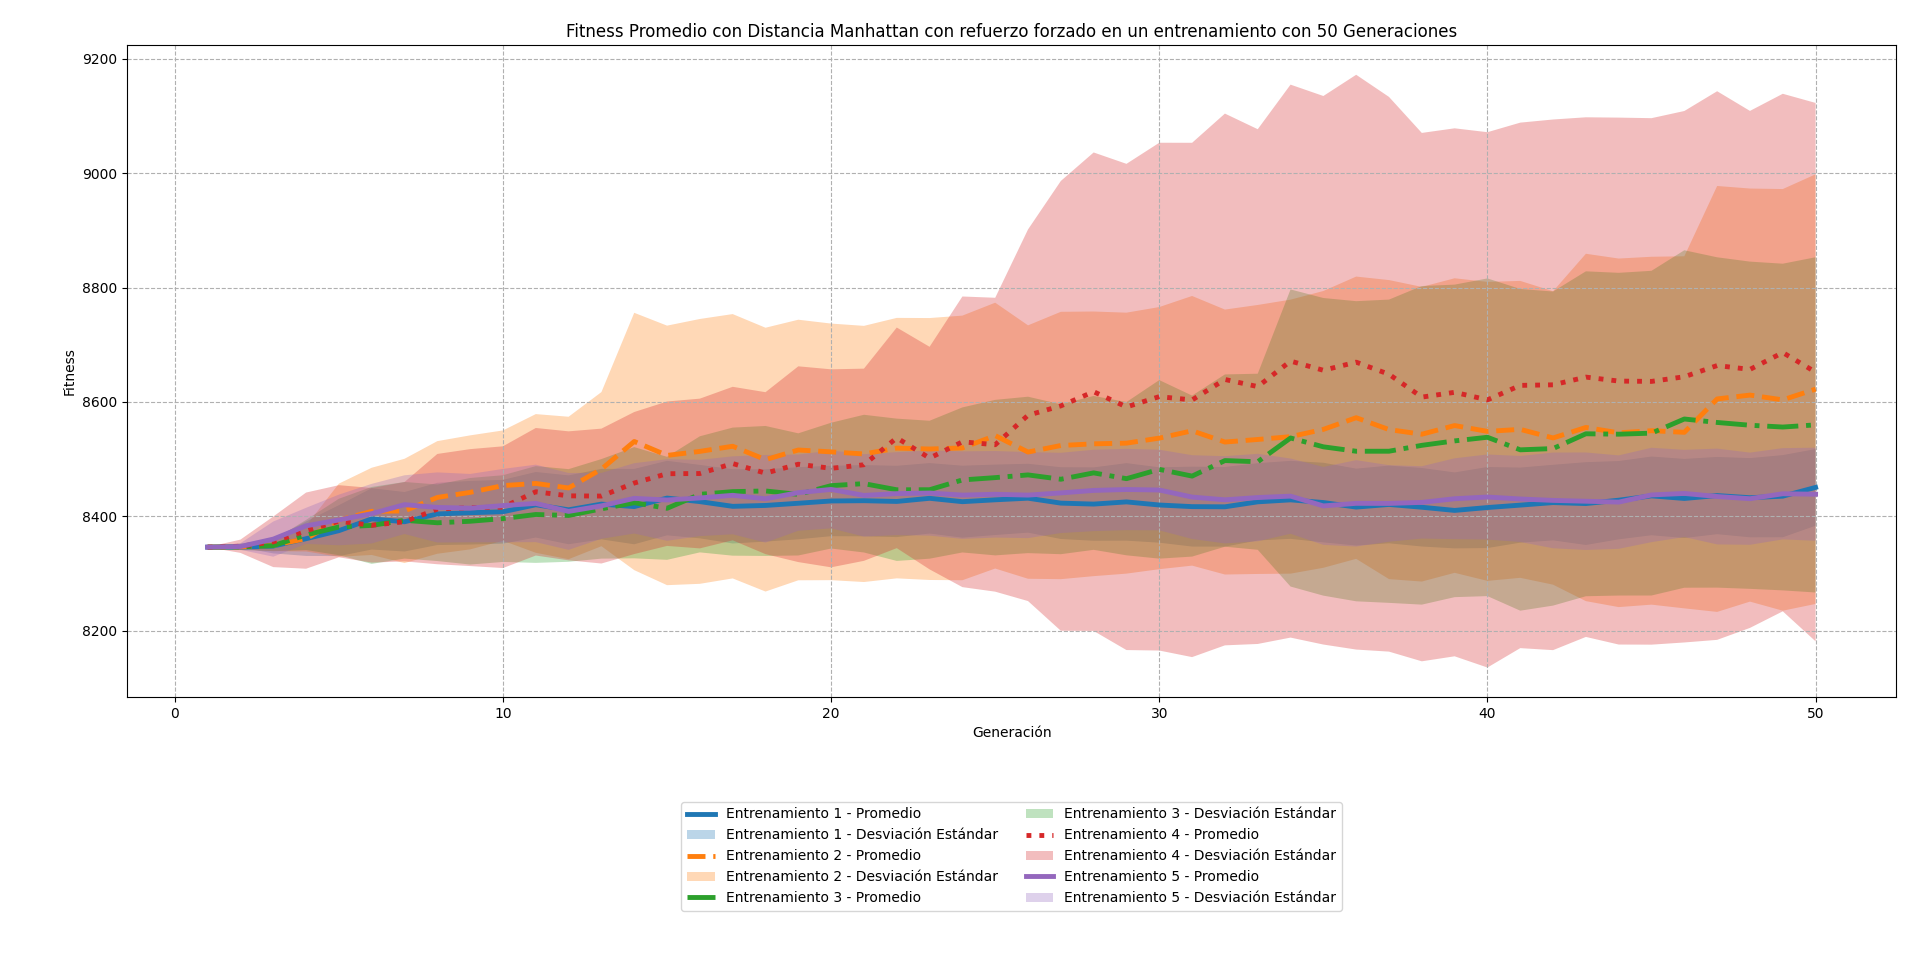
\includegraphics[width=1\linewidth]{Manhattan/Fitness_Acumulado_Manh_50Gen.png}
    \caption{Gráfica de promedios y desviaciones fitness correspondiente a 5
simulaciones realizadas con una generación de 50 para la distancia Manhattan}
    \label{fig:Manhattan_50_genral}
\end{figure}
En el entrenamiento número 4 se presentó el fitness mas alto con 9978 junto con las desviaciones mas altas de todos los entrenamientos, de al rededor de 9100 puntos:
\begin{figure}[H]
    \centering
    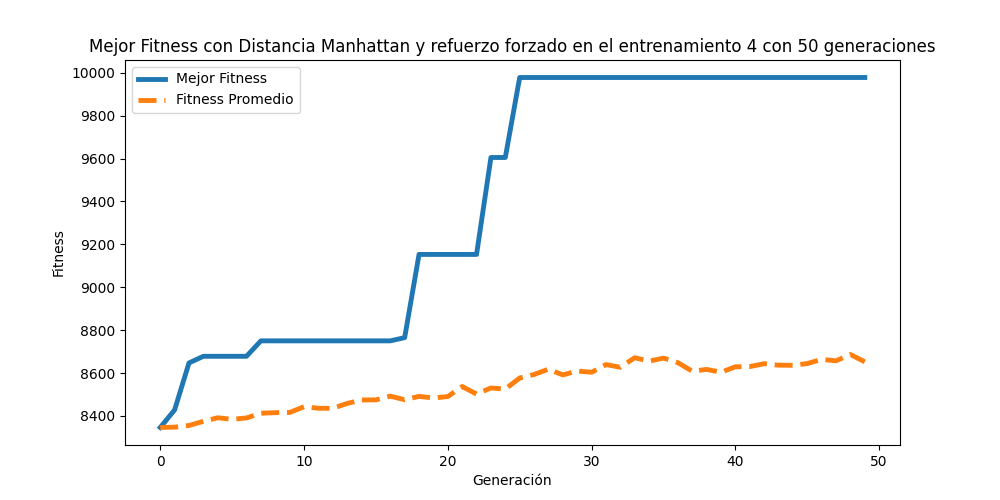
\includegraphics[width=0.9\linewidth]{Manhattan/Fitness_Individual_50Gen/Fitness_4_Manh_50Gen.png}
    \caption{Fitness individual para el entrenamiento 4 de 50 generaciones aplicando la distancia Manhattan}
    \label{fig:Fitnes_man_4_50_inv}
\end{figure}
\begin{figure}[H]
    \centering
    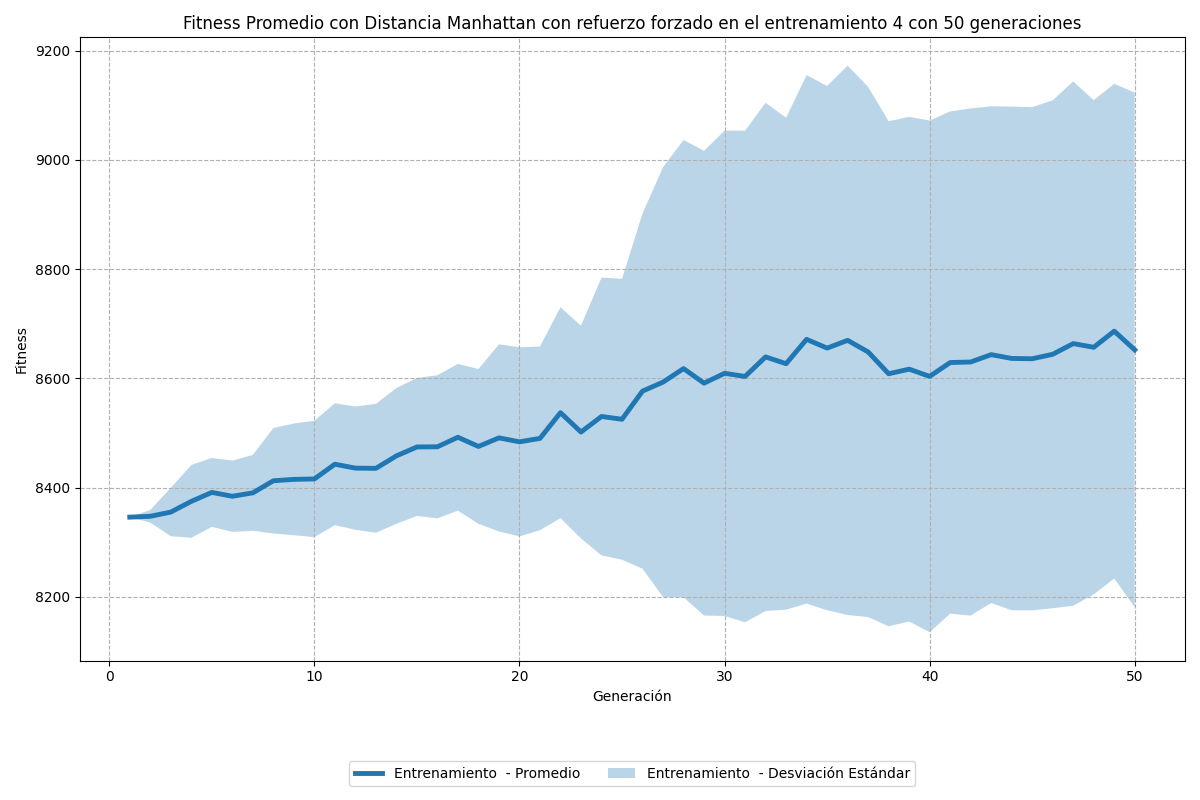
\includegraphics[width=0.9\linewidth]{Manhattan/Fitness_Individual_50Gen/Fitness_4_Manh_50Gen_Sombra.png}
    \caption{Fitness promedio y desviación individual para el entrenamiento 4 de 50 generaciones aplicando la distancia Manhattan}
    \label{fig:Fitnes_ecu_4_50_inv_sombra_1}
\end{figure}
Los sigueientes dos entrenamientos con los puntajes mas altos fueron el 2 y 3, con 9688 y 9621 respectivamente, con una desviación que no supera los 8900 para el entrenamiento numero 3, y 9000 para el entrenamiento numero 2 (Fig. \ref{fig:manhattan_2_50}, \ref{fig:manhattan_2_50_sombra}, \ref{fig:manhattan_3_50} y \ref{fig:manhattan_3_50_sombra}). Por último, el primer y quinto entrenamiento obtuvieron los puntajes mas bajos, con 8767 y 8771, con una desviación que no supera los 8600 (Fig. \ref{fig:manhattan_1_50}, \ref{fig:manhattan_1_50_sombra}, \ref{fig:manhattan_5_50}, \ref{fig:manhattan_5_50_sombra}).


\subsubsection{30 Generaciones}
En la gráfica general para las simulaciones con 30 generaciones se observan los fitness promedio de cada entrenamiento y las desviaciones:
\begin{figure}[H]
    \centering
    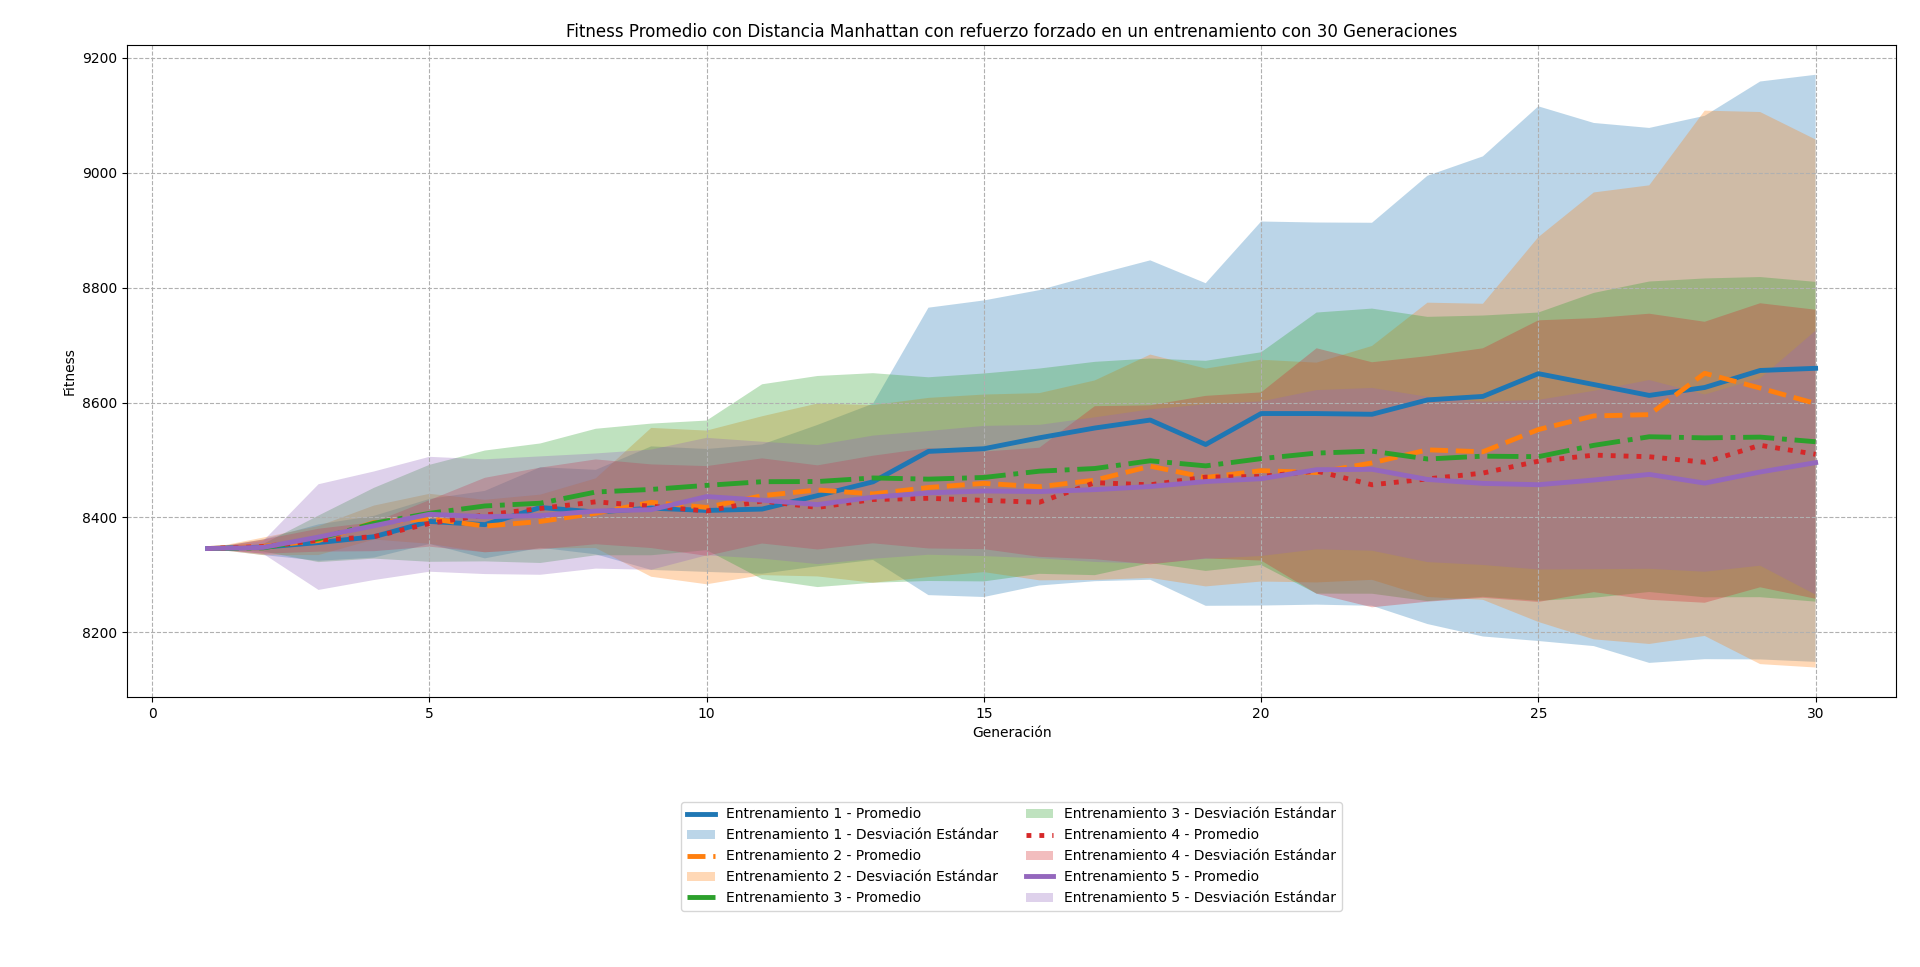
\includegraphics[width=1\linewidth]{Manhattan/Fitness_Acumulado_Manh30Gen.png}
    \caption{Gráfica de promedios y desviaciones para correspondiente a las generaciones de 30 para la distancia Manhattan}
    \label{fig:Manhattan_30_genral}
\end{figure}
%9992
%9989
Los entrenamientos que más fitness obtuvieron durante estas simulaciones, fue el primer y segundo entrenamiento. El puntaje máximo para el primer entrenamiento es de 9990
\begin{figure}[H]
    \centering
    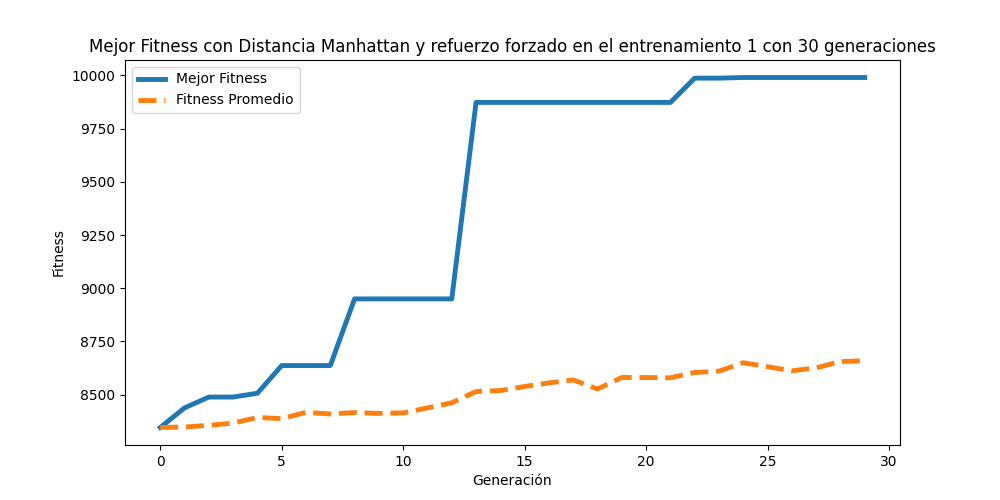
\includegraphics[width=0.99\linewidth]{Manhattan/Fitness_Individual_30Gen/Fitness_1_Mahn_30Gen.png}
    \caption{Fitness promedio y más alto para el entrenamiento 1 de 30 generaciones con la distancia Manhattan}
    \label{fig:manhattan_30_fitness}
\end{figure}
La desviación para el primer entrenamiento ronda los 9100
\begin{figure}[H]
    \centering
    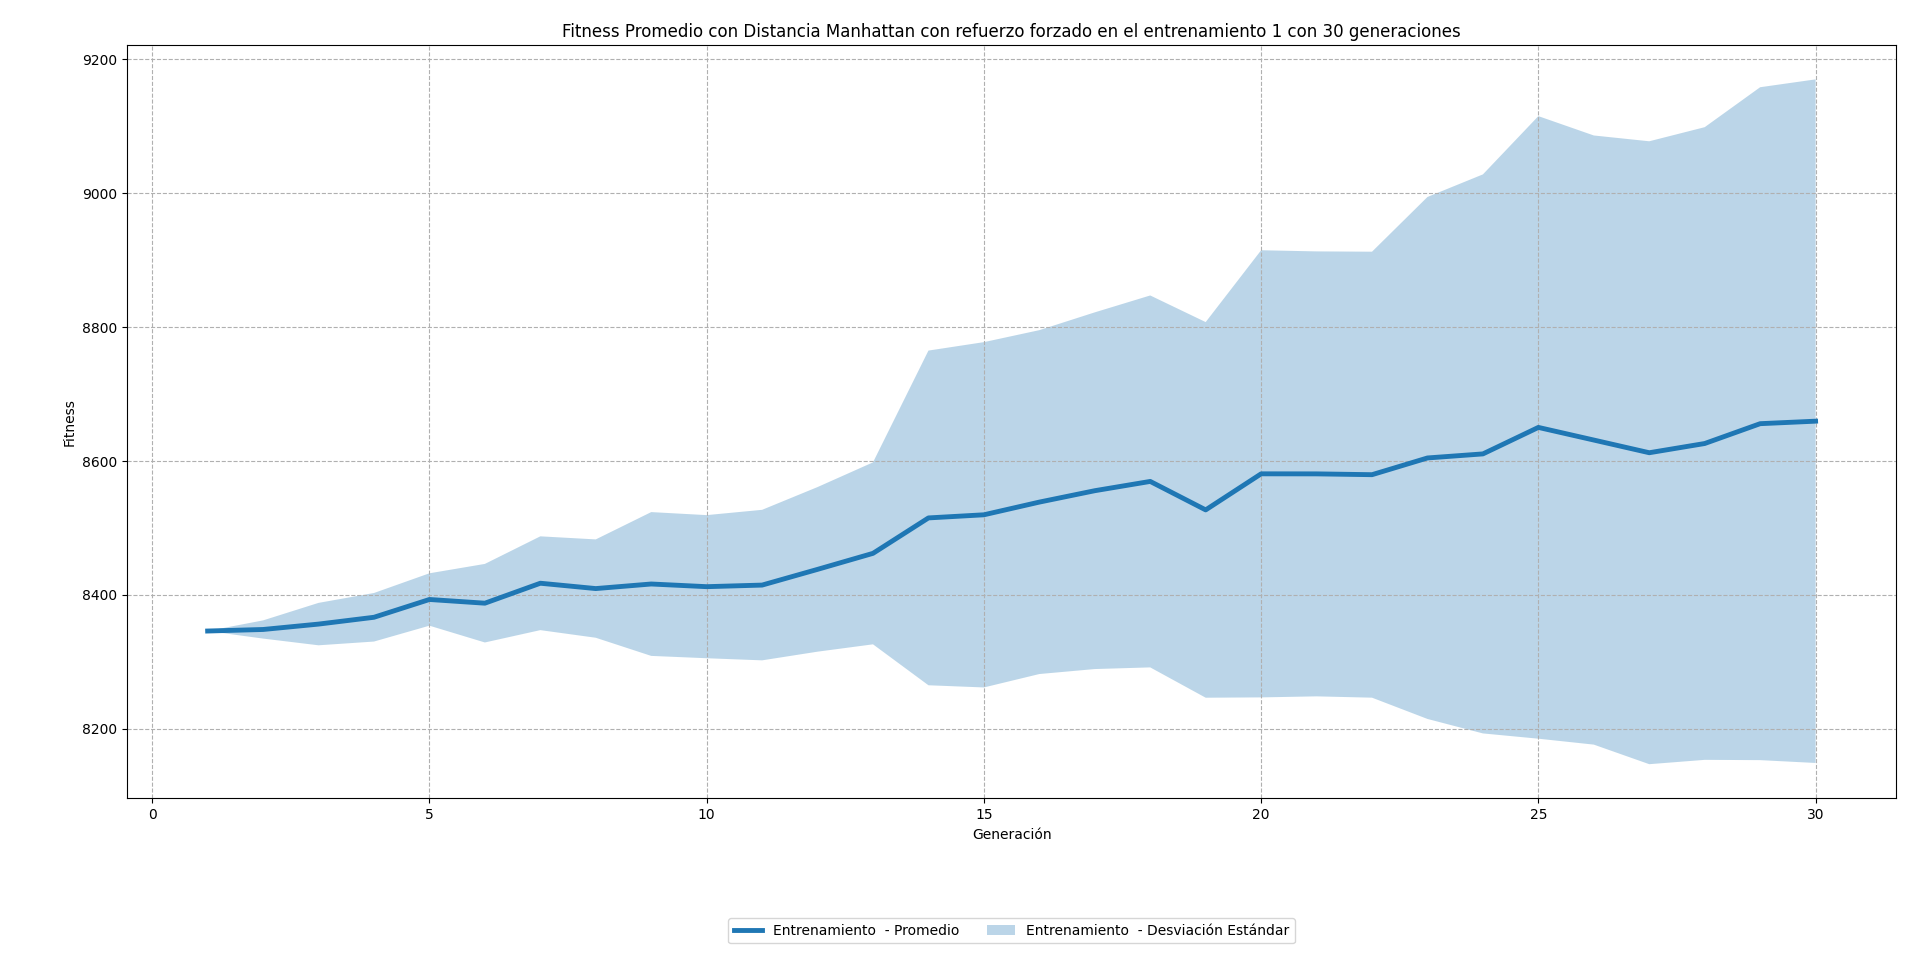
\includegraphics[width=1\linewidth]{Manhattan/Fitness_Individual_30Gen/Fitness_1_Mahn_30Gen_Sombra.png}
    \caption{Fitness promedio y desviación individual para el entrenamiento 1 de 30 generaciones aplicando la distancia Manhattan}
    \label{fig:Fitnes_ecu_1_30_inv_sombra_1-1}
\end{figure}
Para el segundo entrenamento el puntaje máximo es de 9987, superando tambien los 9000 puntos en la desviación, sin embargo en la generación 28 hubo un decremento en el promedio de fitness obtenidos, todo lo contrario al primer entrenamiento (Fig. \ref{fig:manhattan_2_30} y \ref{fig:manhattan_2_30_sombra}). El siguiente mayor puntaje le corresponde al entrenamiento numero 5, este obtuvo un puntaje de 9630, con una desviación que supera los 8700 puntos a partir de la generación 29. Por último, el cuarto y tercer entrenamiento se obtuvieron los puntajes mas bajos, con 9623 y 9618, con una desviación que no supera los 8900 puntos  (Fig. \ref{fig:manhattan_3_30}, \ref{fig:manhattan_3_30_sombra}, \ref{fig:manhattan_4_30} y \ref{fig:manhattan_4_30_sombra}).


\subsubsection{20 Generaciones}
En la gráfica general para las
simulaciones con 20 generaciones se observan los fitness promedio de cada entrenamiento y las desviaciones:
\begin{figure}[H]
    \centering
    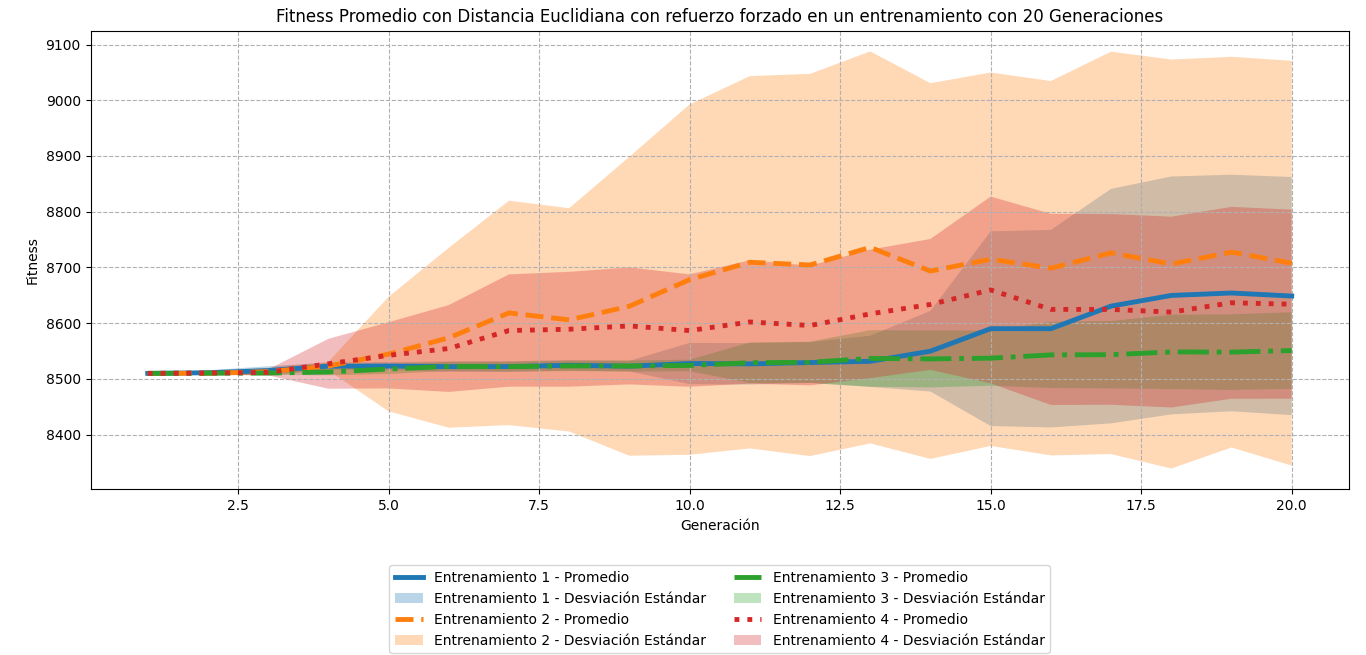
\includegraphics[width=1\linewidth]{Euclidiana/Fitness_Acumulado_Eucli_20Gen.png}
    \caption{Fitness promedio y desviaciones para las simulaciones realizadas con 20 generaciones aplicando la distancia Manhattan}
    \label{fig:manhatan_20_general}
\end{figure}
El entrenamiento número dos obtuvo el mejor fitness, con un puntaje de 9980, su gráfica es:
\begin{figure}[H]
    \centering
    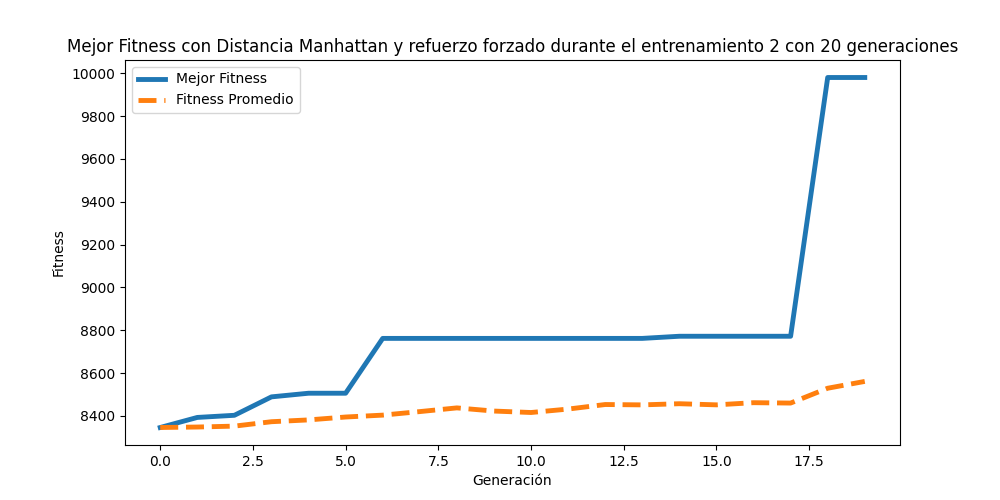
\includegraphics[width=0.99\linewidth]{Manhattan/Fitness_Individual_20Gen/Fitness_2_Manh_20Gen.png}
    \caption{Fitness máximo y promedio para los entrenamientos realizados de 20 generaciones en la distancia Manhattan}
    \label{fig:manhattan20_2}
\end{figure}
Este entrenamiento también posee la mayor desviación de todas
\begin{figure}[H]
    \centering
    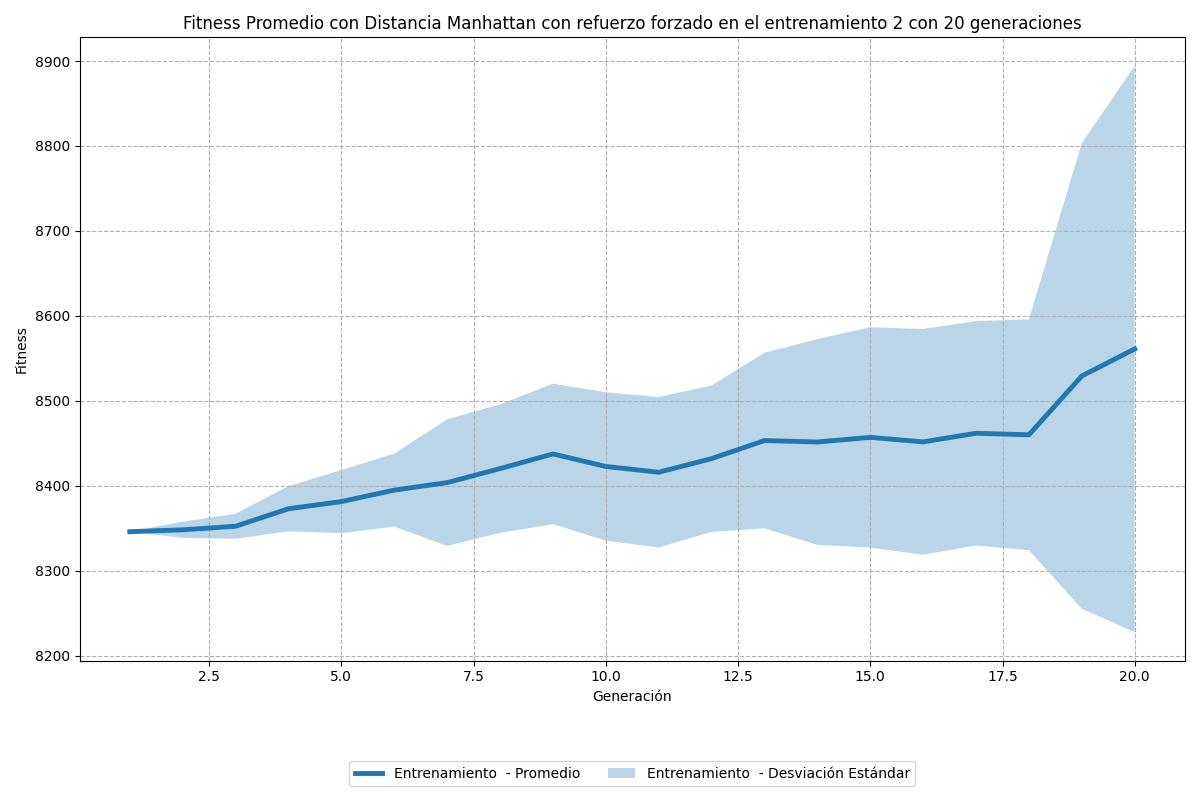
\includegraphics[width=0.99\linewidth]{Manhattan/Fitness_Individual_20Gen/Fitness_2_Manh_20Gen_Sombra.png}
    \caption{Fitnes promedio y desviaciones para el segundo entrenamiento de 20 generaciones  en la distancia Manhattan}
    \label{fig:des_man_2}
\end{figure}

El entrenamiento número 5 obtuvo el segundo mejor fitness, con un puntaje de 9360, con el pasar de cada genración el promedio aumenta, junto con la desviación. En la genración 29 a 30 el puntaje sobrepasó los 8800 (Fig. \ref{fig:manhattan_5_20} y \ref{fig:manhattan_5_20_sombra}). El cuarto entrenamiento obtuvo un puntaje de 8799, con una desviación maxima de 8600, en la generación 19 y 20 el promedio de fitness fue de 8600 puntos (Fig. \ref{fig:manhattan_4_20} y \ref{fig:manhattan_4_20_sombra}). Por último, el primer y tercer entrenamiento obtuvieron los puntajes mas bajos, con 8782 y 8771, con una desviación que sobrepasa los 8600 puntos en la genración numero 15. Por último los peores puntajes fueron obtenidos por el tercer y primer entrenamiento, con un puntaje de 8771, y 8766 respectivamente, ambas superan una desviación de 8600 puntos, de igualmanera comparten una disminución del fitness promedio en la generación 19 y 20 (Fig. \ref{fig:manhattan_3_20}, \ref{fig:manhattan_3_20_sombra},  \ref{fig:manhattan_1_20} y \ref{fig:manhattan_1_20_sombra}).

\subsection{Resultados de las simulaciones aplicando la distancia de Chebyshev}
\subsubsection{50 Generaciones}
De las simulaciones realizadas aplicando la distancia Chebyshev, se obtienen los mejores fitness y promedios, además de todas las desviaciones realizadas en estas
\begin{figure}[H]
    \centering
    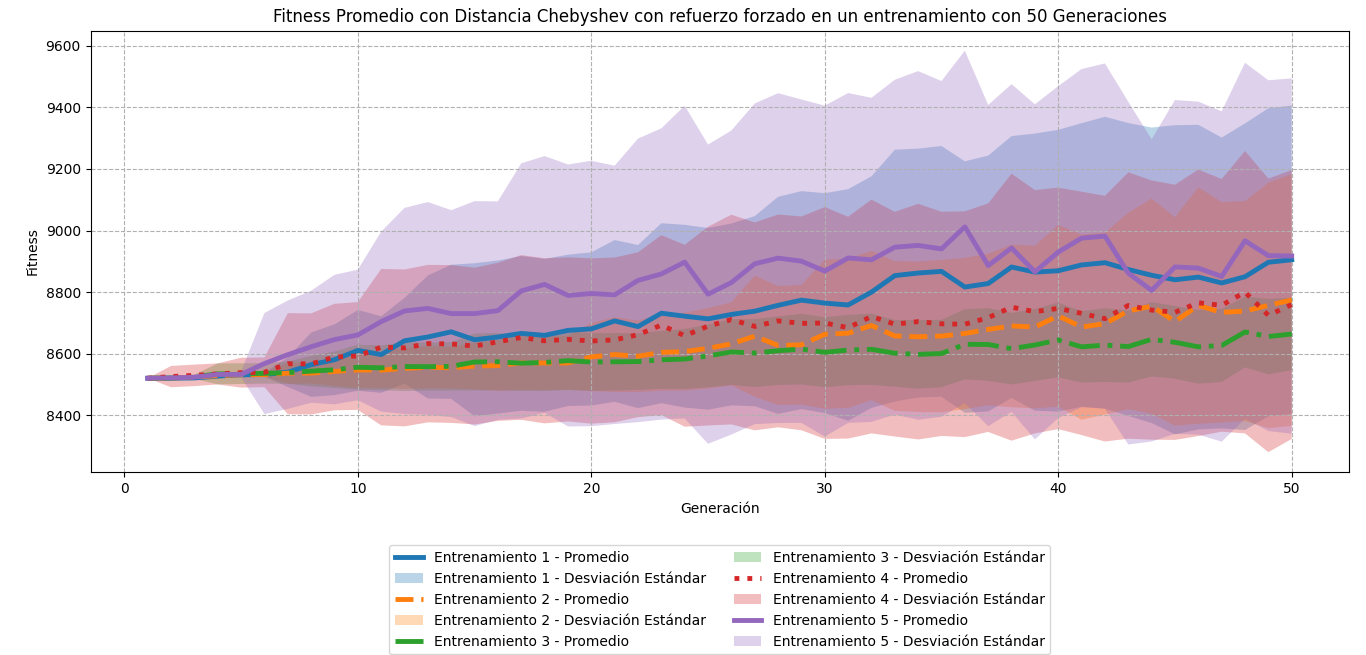
\includegraphics[width=1\linewidth]{Chebyshev/Fitness_Acumulado_Cheby_50Gen.png}
    \caption{Fitness promedio y desviaciones para las simulaciones realizadas con 50 generaciones aplicando la distancia de Chebyshev}
    \label{fig:chy_genral}
\end{figure}
Analizando la gráfica, los valores fitness más altos corresponden al entrenamiento 1 y 5. Por un lado el entrenamiento número 1 presenta el mayor puntaje con 9988:
\begin{figure}[H]
    \centering
    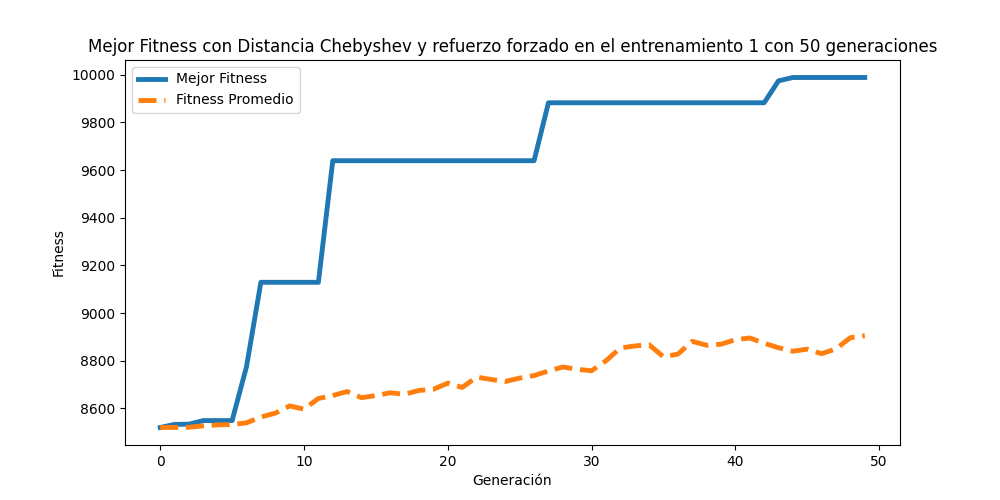
\includegraphics[width=0.9\linewidth]{Chebyshev/Fitness_Individual_50Gen/Fitness_1_Cheby_50Gen.png}
    \caption{Mejor fitness para una generación de 50 aplicando la distancia de Chebyshev}
    \label{fig:chy_1_best}
\end{figure}
Mientras que el puntaje para el entrenamiento 5 es de 9986
\begin{figure}[H]
    \centering
    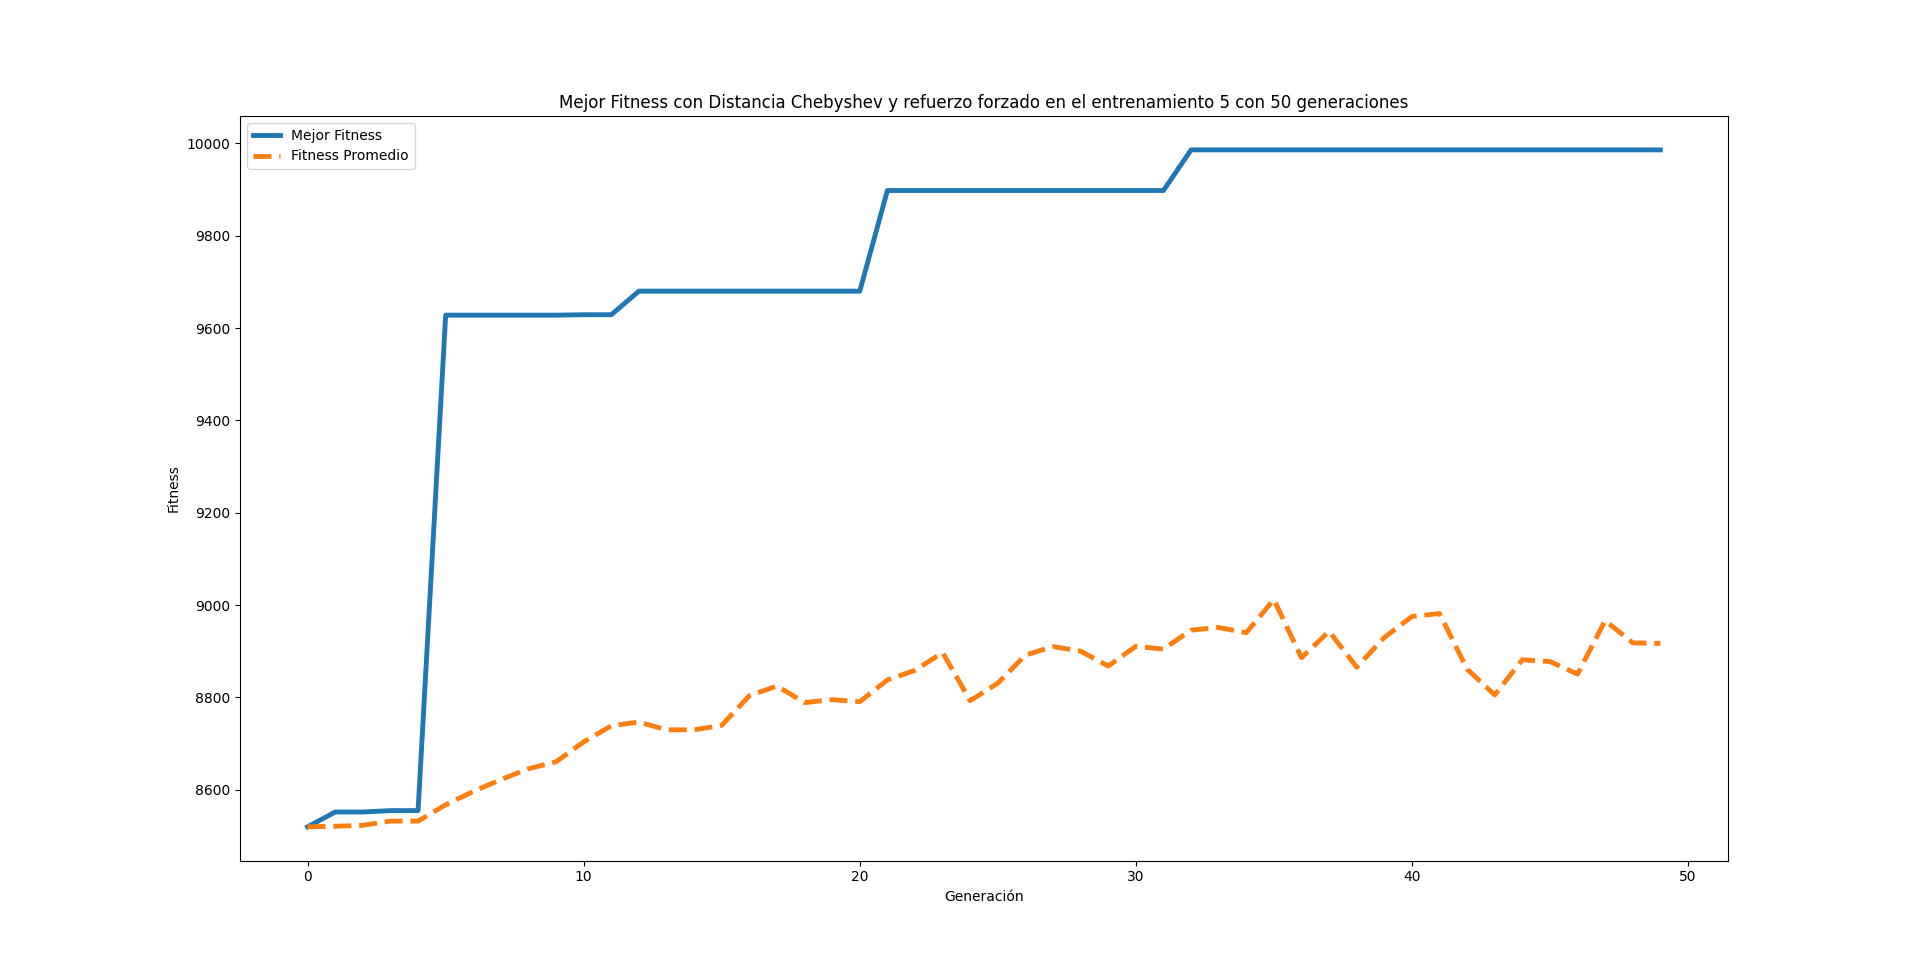
\includegraphics[width=0.9\linewidth]{Chebyshev/Fitness_Individual_50Gen/Fitness_5_Cheby_50Gen.png}
    \caption{Mejor fitness para el entrenamiento 5 de una generación de 50 aplicando la distancia de Chebyshev}
    \label{fig:chy_5_best}
\end{figure}
Sin embargo en este caso particular la mayor desviación la posee el entrenamiento número 5
\begin{figure}[H]
    \centering
    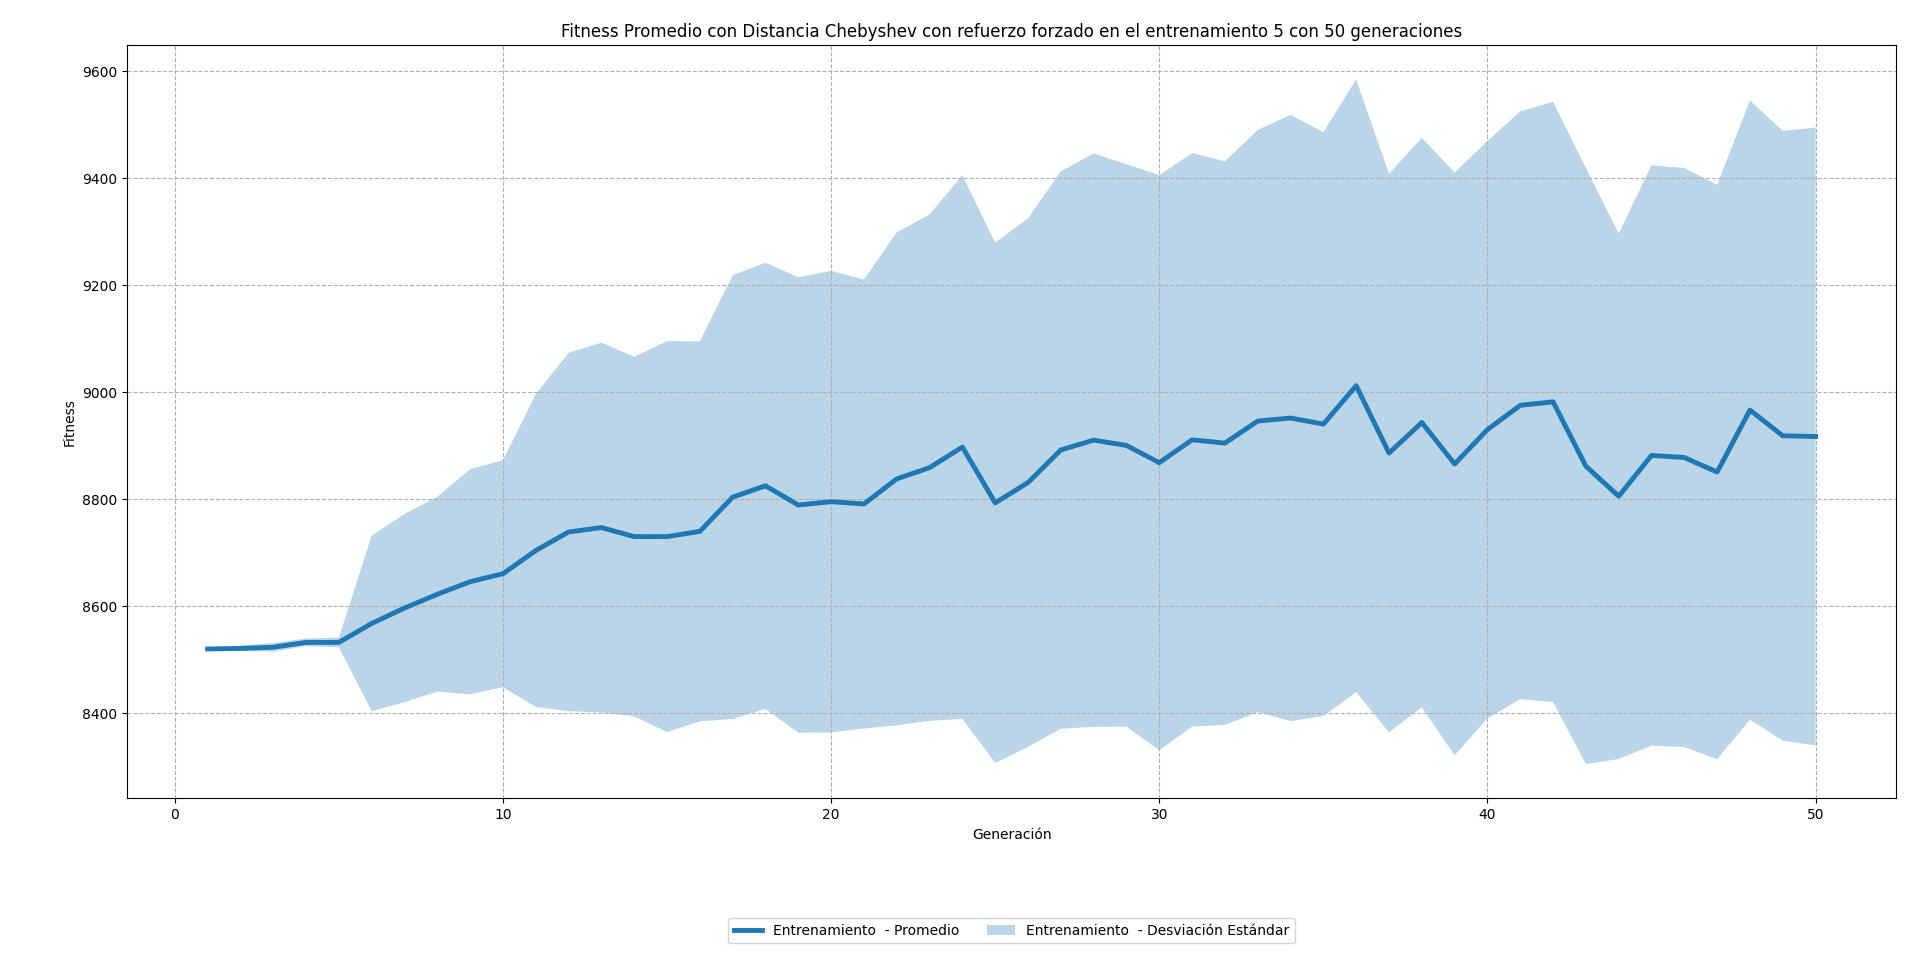
\includegraphics[width=0.9\linewidth]{Chebyshev/Fitness_Individual_50Gen/Fitness_5_Cheby_50Gen_Sombra.png}
    \caption{Mayor desviación en el entrenamiento numero 5, para una generación de 50 con la distancia de Chebyshev}
    \label{fig:che_5_desv}
\end{figure}
Mientras que el entrenamiento número 1 obtuvo una desviación de 9400 puntos en la generación 50, el entrenamiento numero 5 sobrepasa esa desviación a partir de la generación 30. Por otro lado, el entrenamiento número 4, obtuvo el tercer mejor fitness con 9984, acercandose a 9200 puntos en la desviación maxima para la generación 48. Los menores fitness obtenidos fueron para el segundo y tercer entrenamiento, con 9973 y 8777 respectivamente, ambos con una desviación que no supera los 9200 puntos (Fig. \ref{fig:cheb_1_50_sombra}, \ref{fig:cheb_4_50}, \ref{fig:cheb_4_50_sombra}, \ref{fig:cheb_2_50}, \ref{fig:cheb_2_50_sombra}, \ref{fig:cheb_3_50} y \ref{fig:cheb_3_50_sombra}).

\subsubsection{30 Generaciones}
La gráfica general que representa a todos los entrenamientos realizados para la generación de 30 es:
\begin{figure}[H]
    \centering
    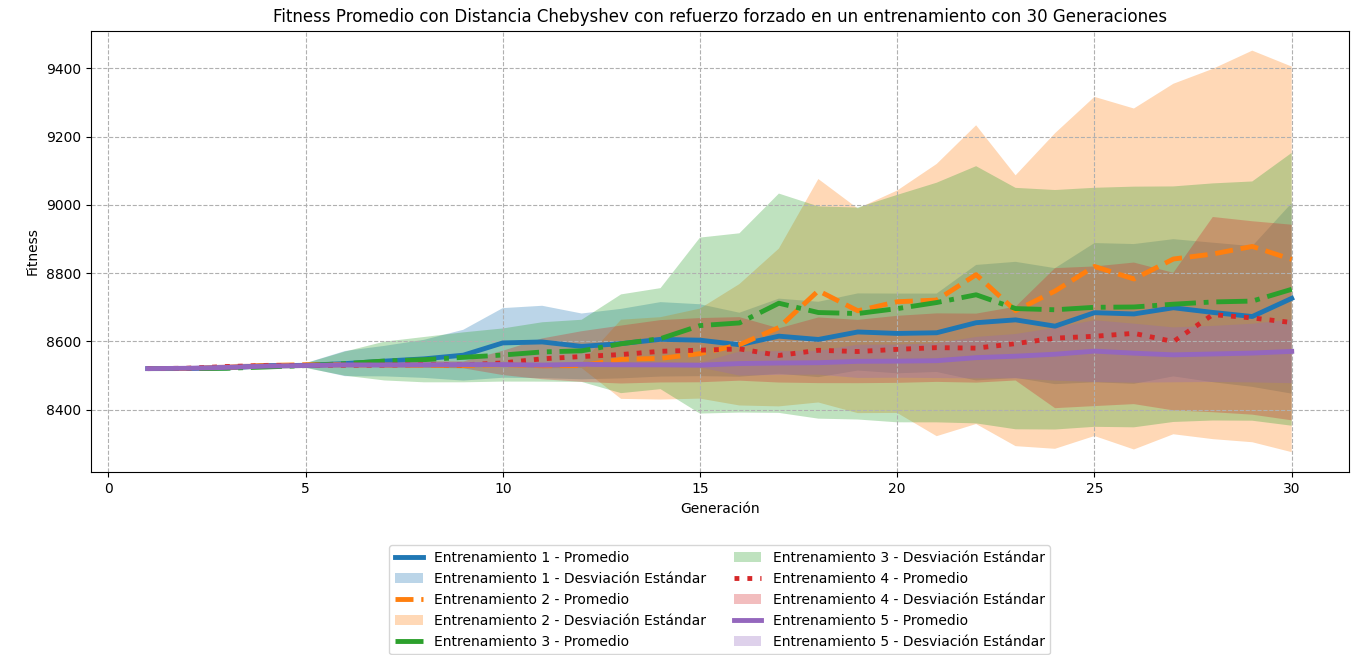
\includegraphics[width=1\linewidth]{Chebyshev/Fitness_Acumulado_Cheby30Gen.png}
    \caption{Fitness promedios y desviaciones de cada entrenamiento realizado para las generaciones de 30 con la distancia de Chebyshev}
    \label{fig:genral_che_30}
\end{figure}
Tanto el entrenamiento numero 2 y 3 presenta el fitness más alto, el segundo entrenamiento posee un valor fitness máximo de 9994, mientras que el tercer entrenamiento uno de 9974
\begin{figure}[H]
    \centering
    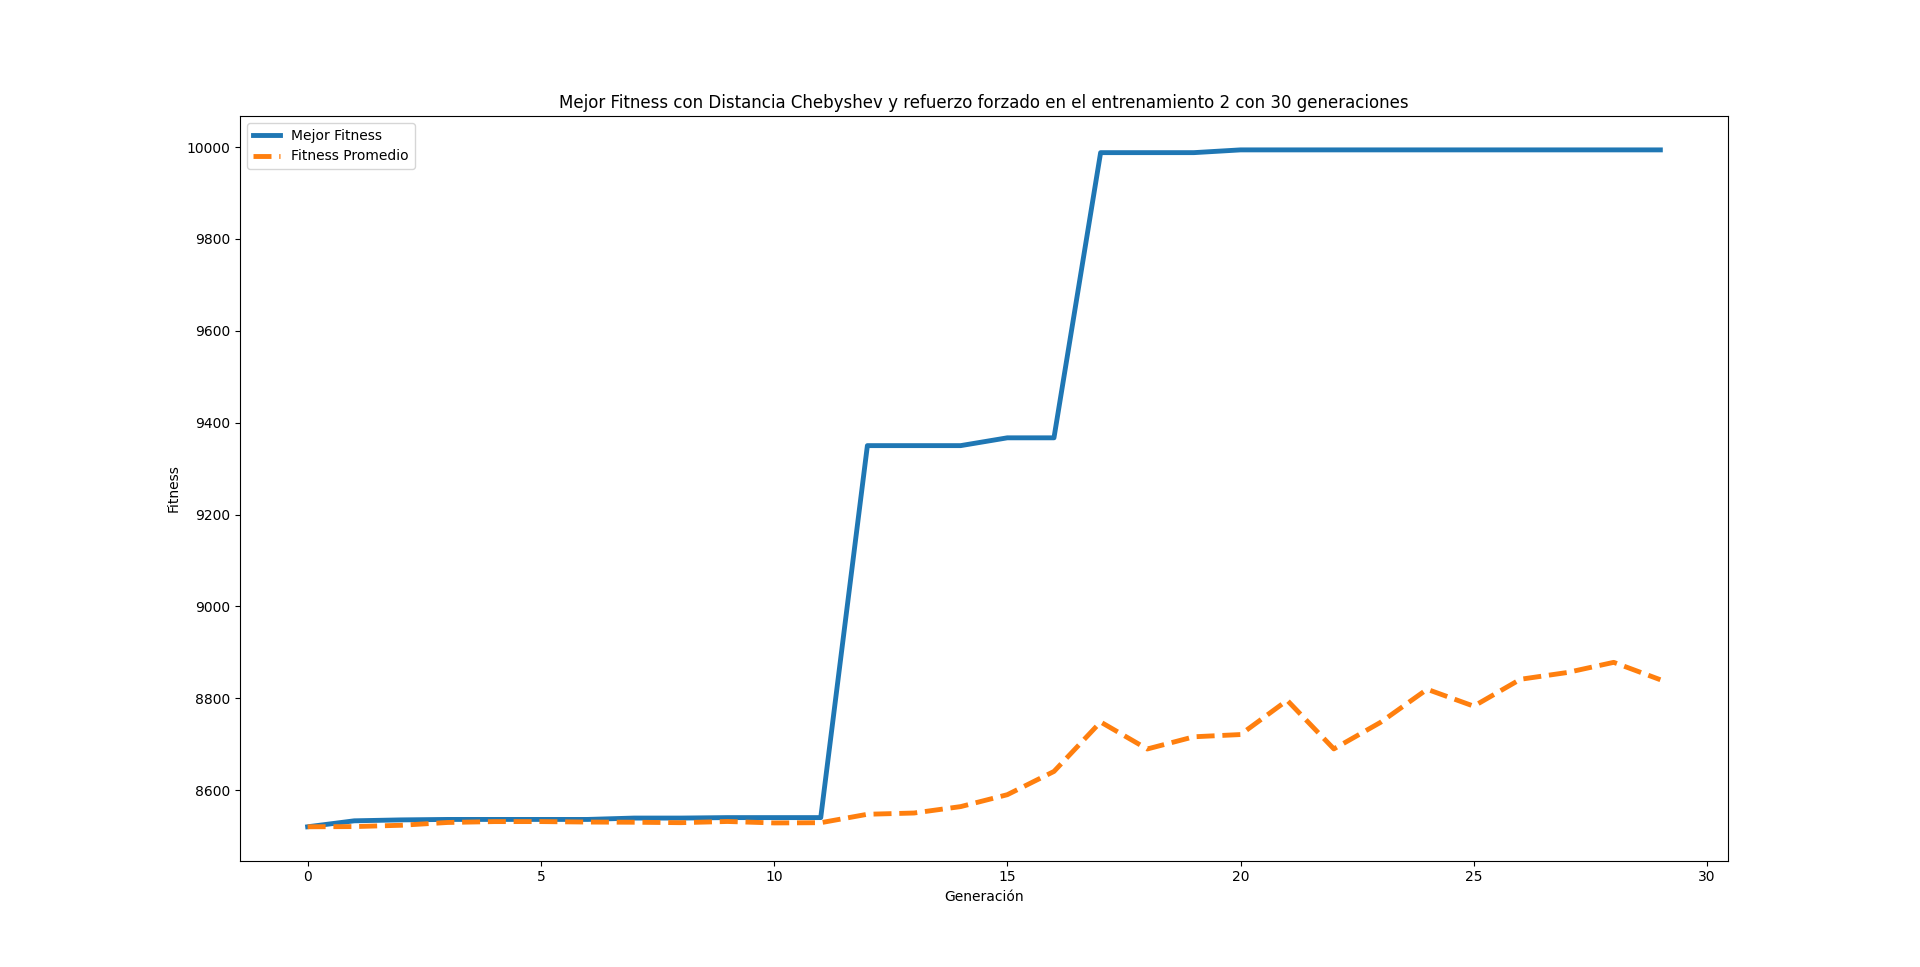
\includegraphics[width=0.99\linewidth]{Chebyshev/Fitness_Individual_30Gen/Fitness_2_Cheby_30Gen.png}
    \caption{Fitness máximo y promedio del segundo entrenamiento para 30 generaciones de la distancia Shebyshev}
    \label{fig:en:she_2}
\end{figure}
\begin{figure}[H]
    \centering
    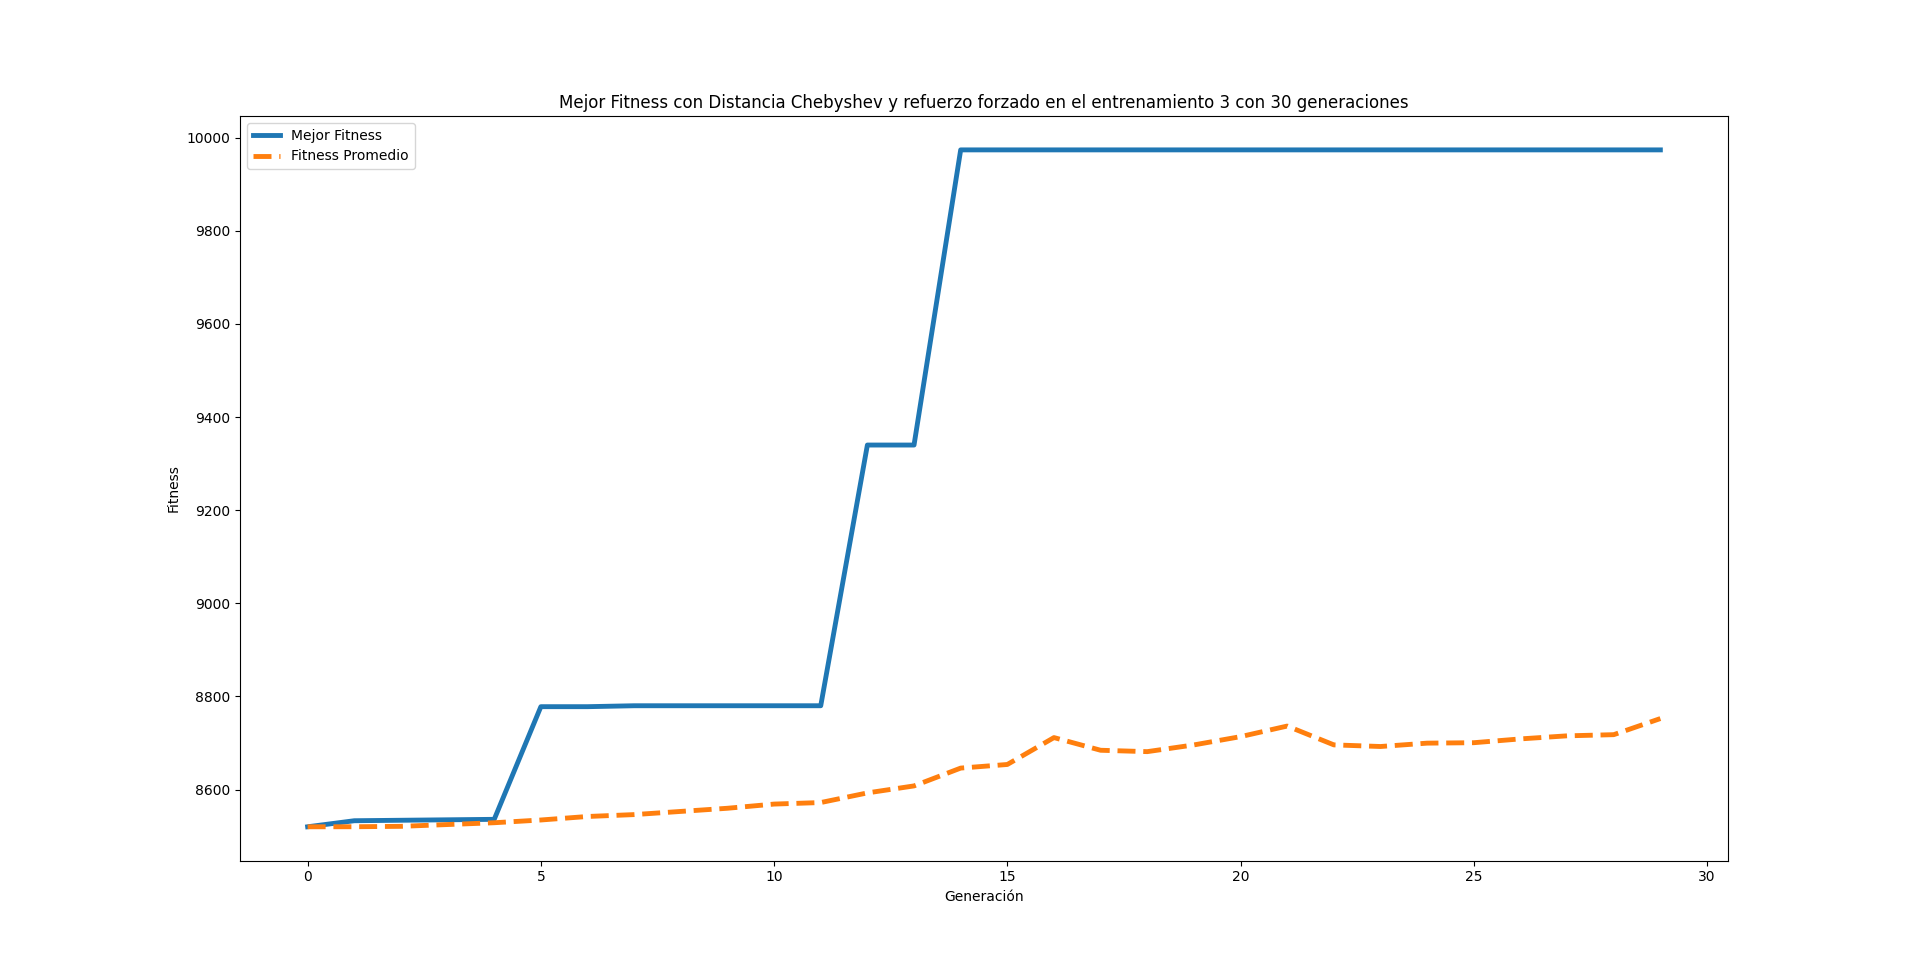
\includegraphics[width=0.99\linewidth]{Chebyshev/Fitness_Individual_30Gen/Fitness_3_Cheby_30Gen.png}
    \caption{Fitness máximo y promedio del tercer entrenamiento para 30 generaciones de la distancia Shebyshev}
    \label{fig:en:she_3}
\end{figure}
La mayor desviación le corresponde al entrenamiento número dos, su gráfica es:
\begin{figure}[H]
    \centering
    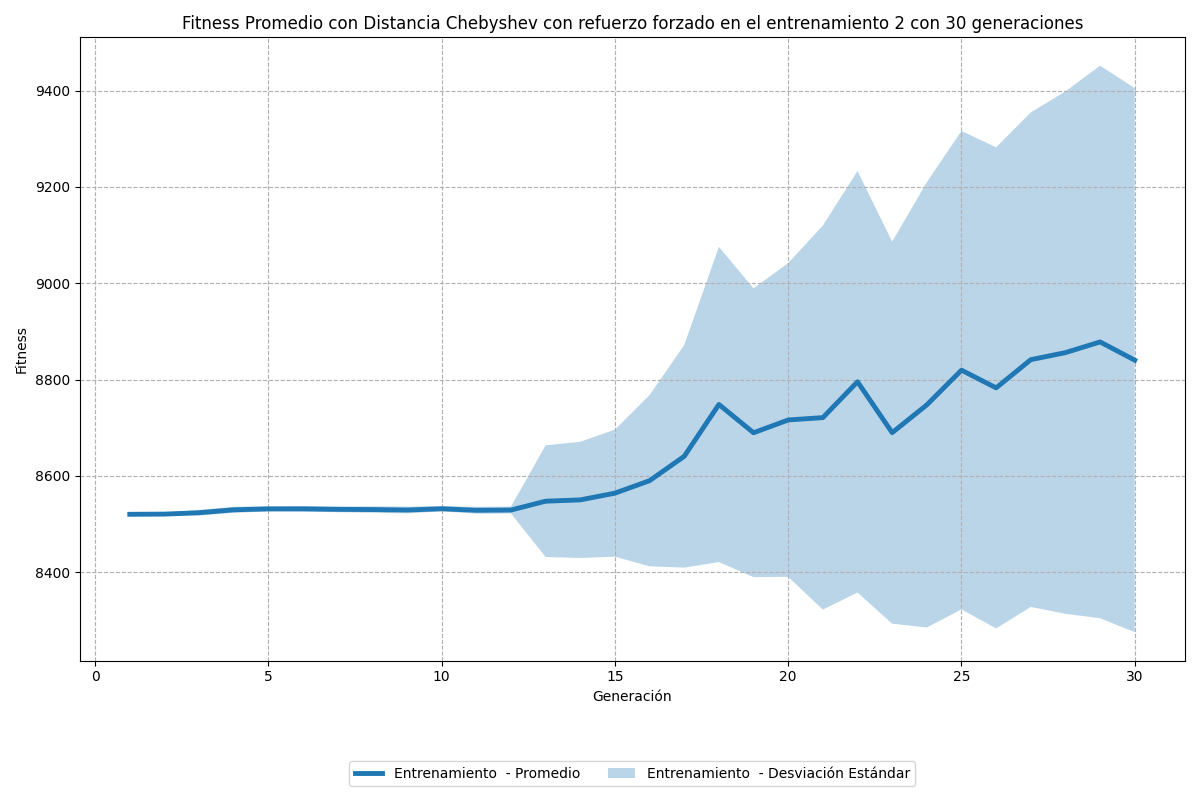
\includegraphics[width=0.99\linewidth]{Chebyshev/Fitness_Individual_30Gen/Fitness_2_Cheby_30Gen_Sombra.png}
    \caption{Mayor desviación para las simulaciones realizadas con las distancia de Chebyshev y 30 generaciones}
    \label{fig:enter-label}
\end{figure}

El entrenamiento numero 3 apenas supera el puntaje de desvición 9100 en su última generación, pero tambien en esta última aumenta ligeramente su promedion em comparación con el segudo entrenamiento. Por otro lado, el cuarto entrenamiento obtuvo el tercer mejor fitness con 9884, con una desviación que no supera los 9000 puntos en la generación 30. Los fitness mas bajos se los llevan el primer y quinto entrenamiento, con 9665 puntos y 8787 respectivamente, ambbos con aumento en el fitnes promedios en la ultima generación (Fig. \ref{fig:cheb_2_30_sombra}, \ref{fig:cheb_3_30},  \ref{fig:cheb_3_30_sombra}, \ref{fig:cheb_4_30}, \ref{fig:cheb_4_30_sombra}, \ref{fig:cheb_5_30} y \ref{fig:cheb_5_30_sombra}).


\subsubsection{20 Generaciones}
En la gráfica general para las
simulaciones con 20 generaciones se observan los fitness promedio de cada entrenamiento y las desviaciones:
\begin{figure}[H]
    \centering
    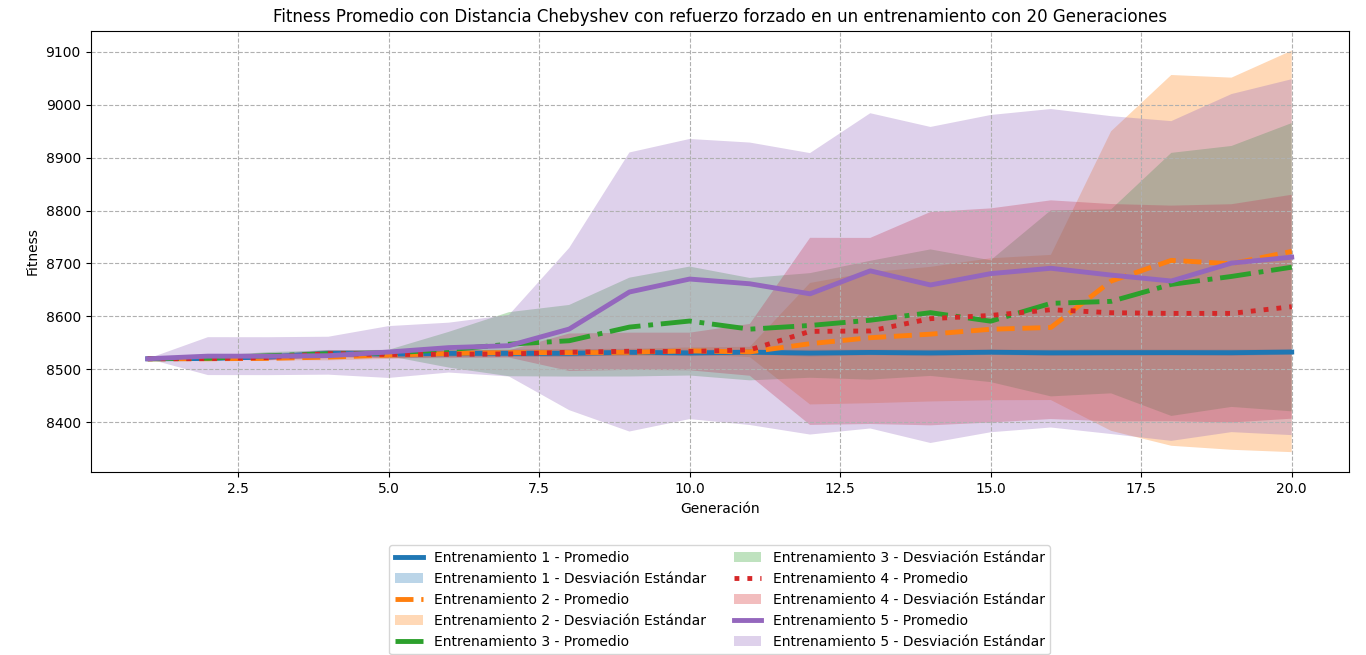
\includegraphics[width=1\linewidth]{Chebyshev/Fitness_Acumulado_Cheby_20Gen.png}
    \caption{Fitness y desviaciones generales de los entrenamientos realizados para una generación de 20 con la distancia Chebyshev}
    \label{fig:chy_20:genral}
\end{figure}
El entrenamiento con mayor fitness en este caso también posee la mayor desviación, el entrenamiento número dos obtuvo un fitness máximo de 9990
\begin{figure}[H]
    \centering
    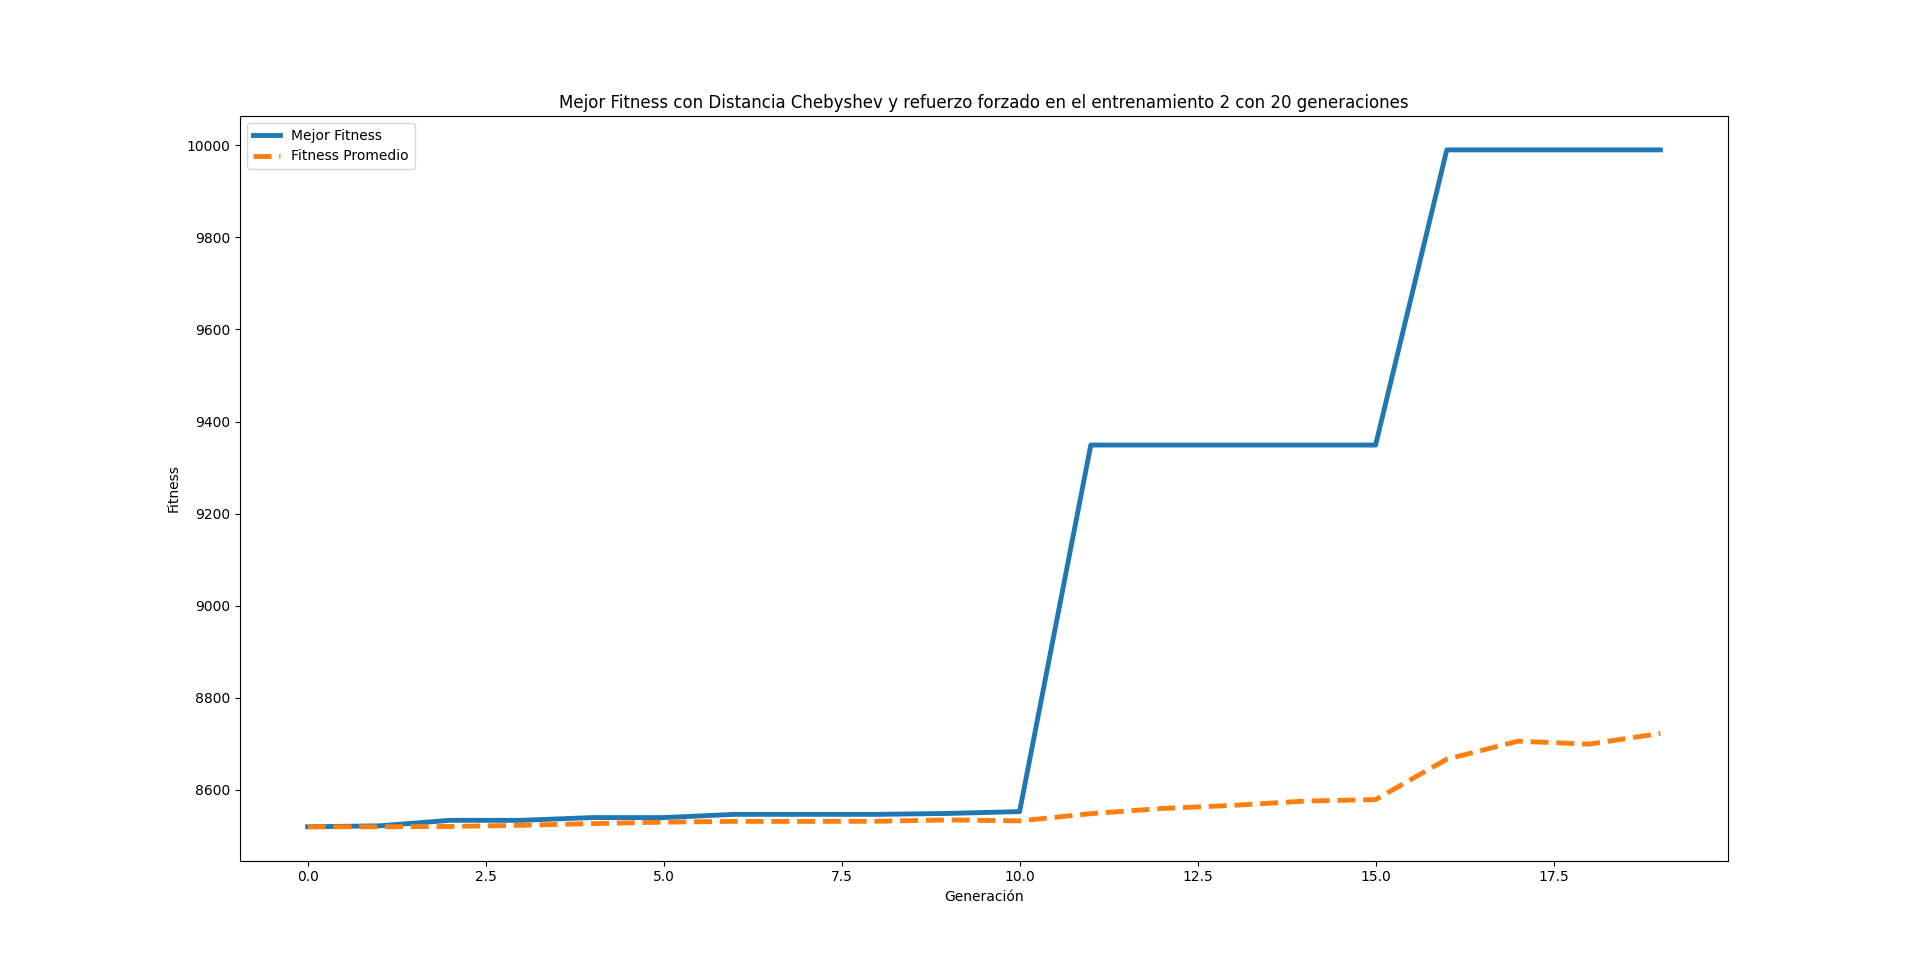
\includegraphics[width=0.99\linewidth]{Chebyshev/Fitness_Individual_20Gen/Fitness_2_Cheby_20Gen.png}
    \caption{Fitnes máximo y promedio para una generación de 20 con la distancia de Chebyshev}
    \label{fig:max_cheby_20g}
\end{figure}
\begin{figure}[H]
    \centering
    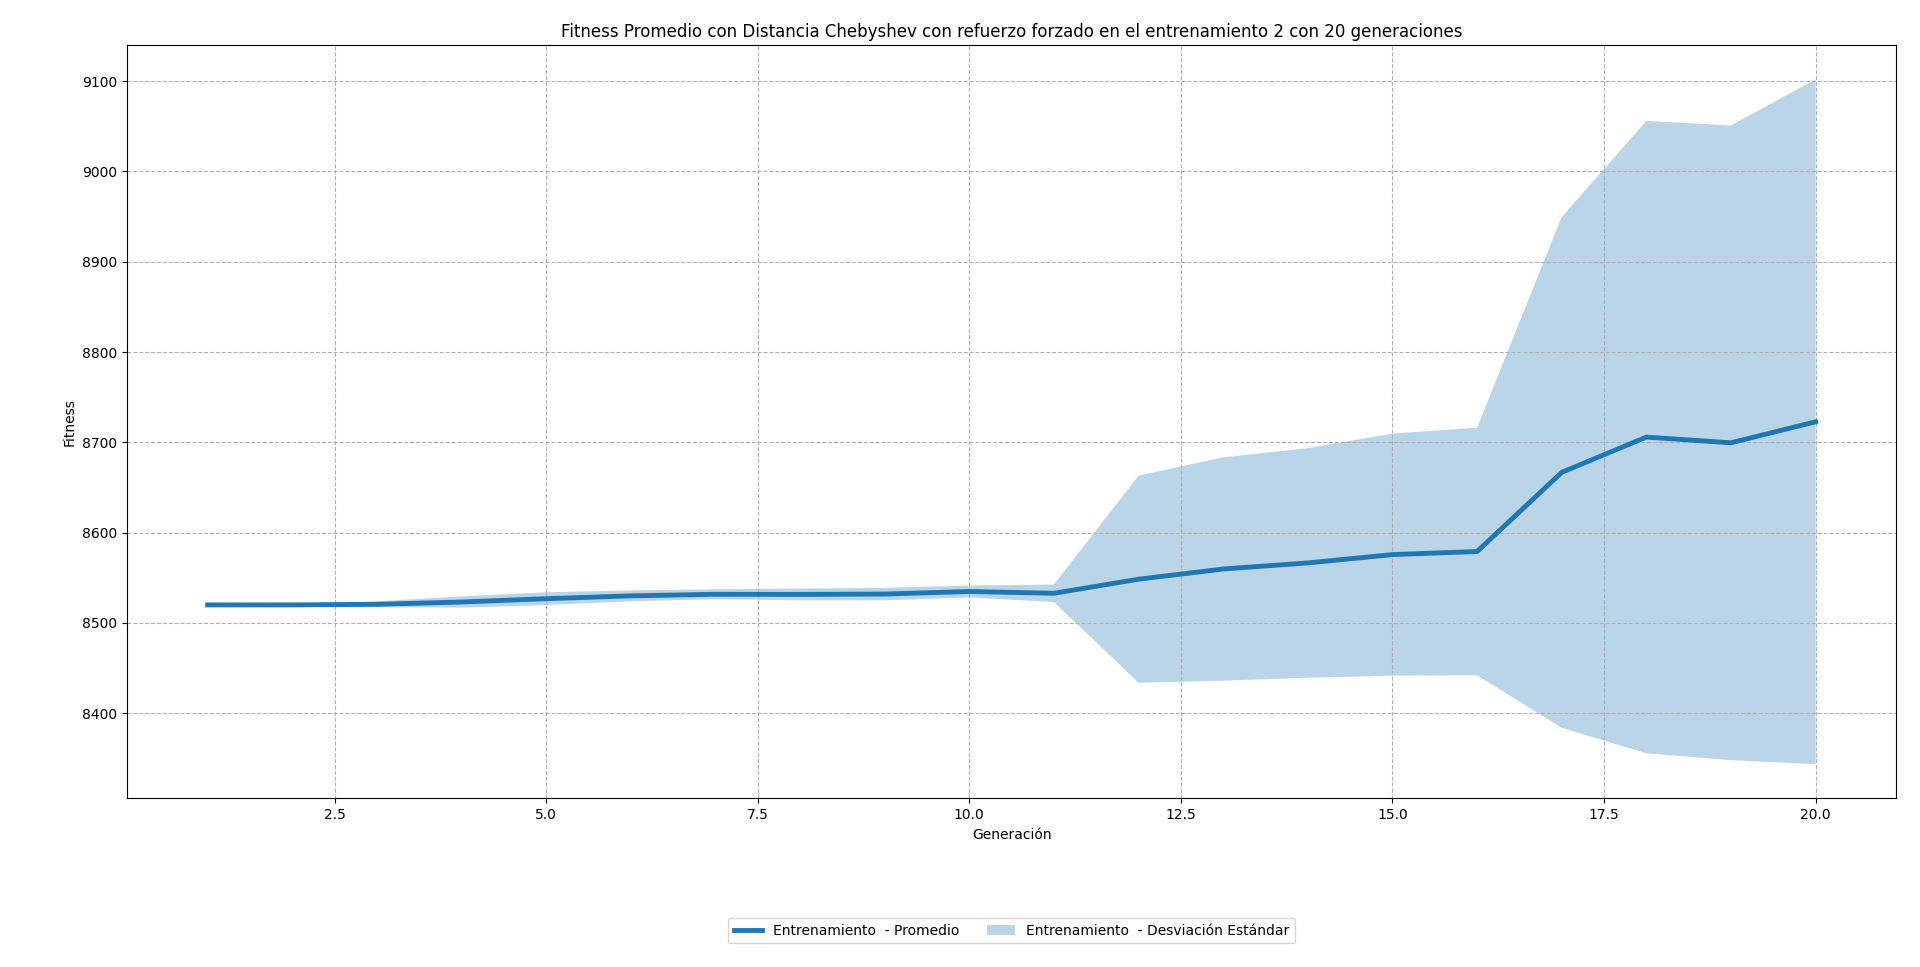
\includegraphics[width=0.99\linewidth]{Chebyshev/Fitness_Individual_20Gen/Fitness_2_Cheby_20Gen_Sombra.png}
    \caption{Fitnes promedio y desviaciones del entrenamiento 2 correspondiente a la distancia Chebyshev para una generación de 20}
    \label{fig:ind_20_chevy}
\end{figure}
El entrenamiento número 3 obtuvo el segundo mejor resultado con un puntaje fitness máximo de 9906
\begin{figure}[H]
    \centering
    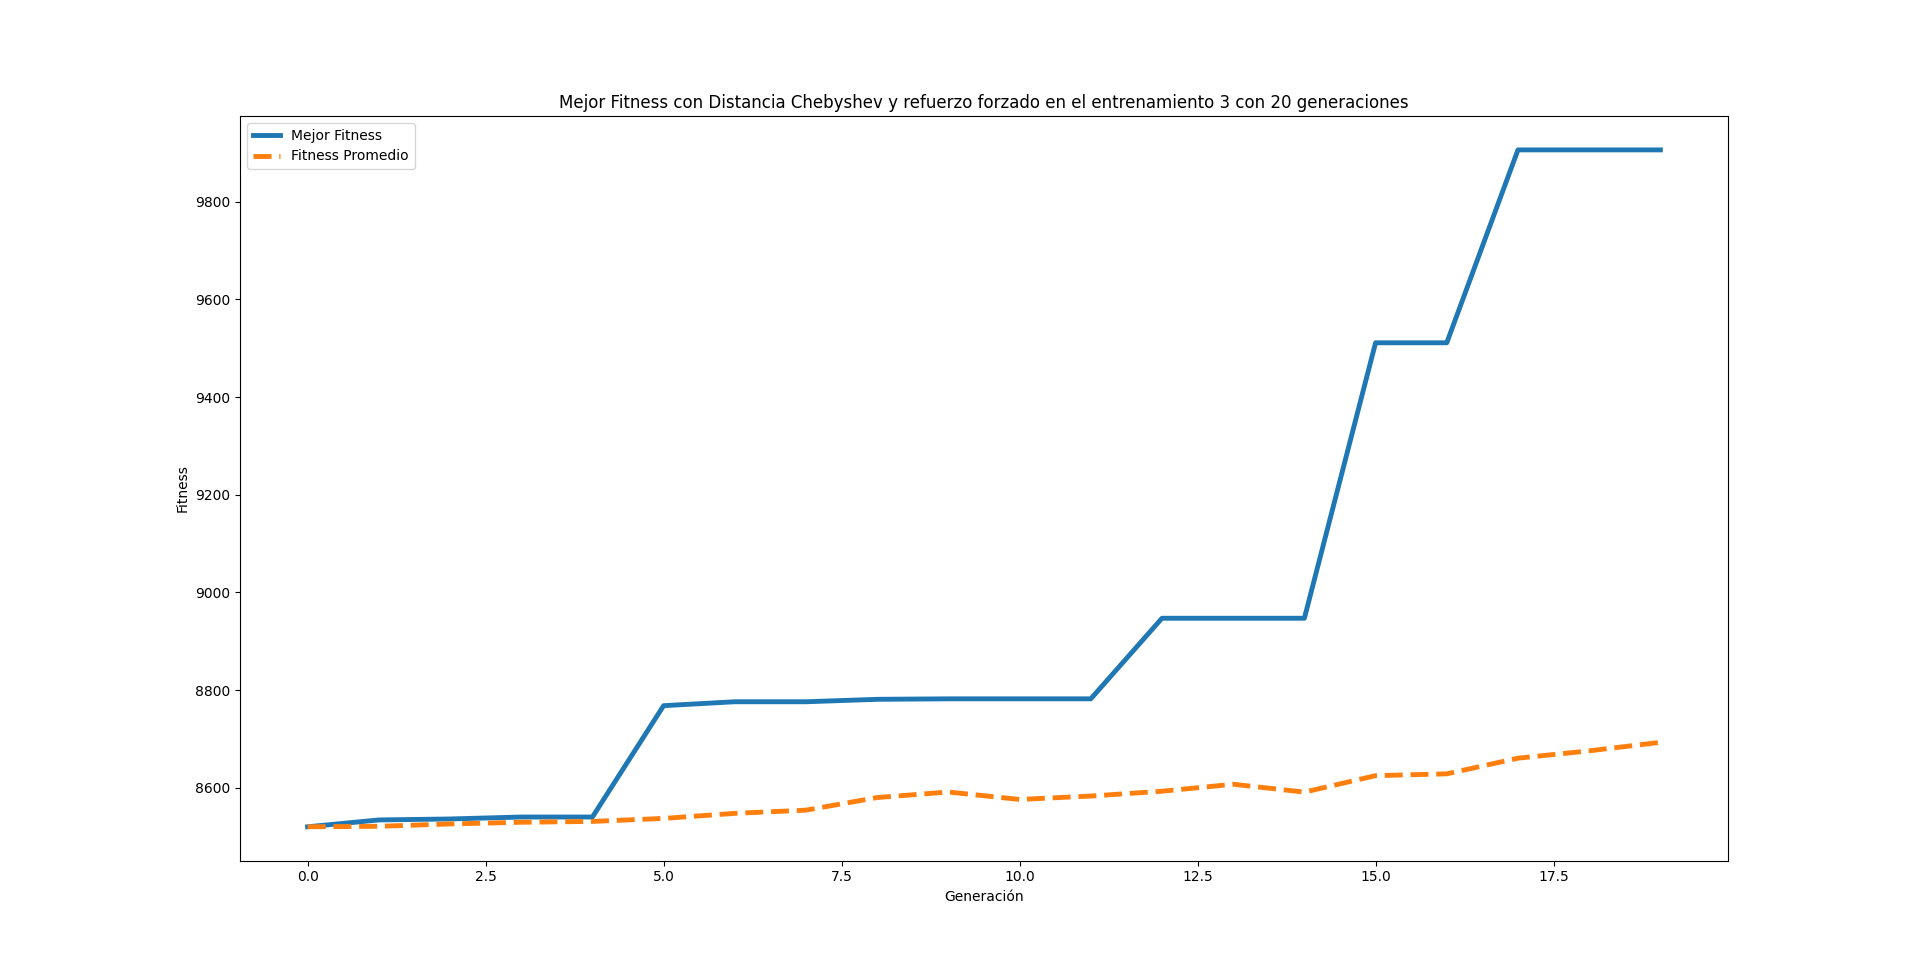
\includegraphics[width=0.99\linewidth]{Chebyshev/Fitness_Individual_20Gen/Fitness_3_Cheby_20Gen.png}
    \caption{Fitnes máximo y promedio para una generación de 20 con la distancia de Chebyshev en el tercer entrenamiento}
    \label{fig:max_cheby3_20g}
\end{figure}
Además el quinto entrenamiento obtuvo 9882 como puntaje máximo fitness, los fitness mas bajos se los llevan el primer y cuarto entrenamiento, con 8543 y 9680 respectivamente. Sin embargo estos últmios tres entrenamientos en la ultima gneración incrementaron el fitness promedio (Fig. \ref{fig:cheb_1_20}, \ref{fig:cheb_1_20_sombra}, \ref{fig:cheb_4_20},
\ref{fig:cheb_3_20_sombra},
\ref{fig:cheb_4_20_sombra}, \ref{fig:cheb_5_20}, \ref{fig:cheb_5_20_sombra}).

\subsection{50 generaciones sin el Refuerzo forzado o Método de aceleración}
Para esta sección solo se realizó un entrenamiento con el fin de ver que tan optimo era realizar las simulaciones sin la aplicación del método descrito en la Figura \ref{fig:reforce}.
% Ch 9885
% mah 8535
En la aplicación de la distancia Euclidiana el mayor fitness obtenido es de 8536
\begin{figure}[H]
    \centering
    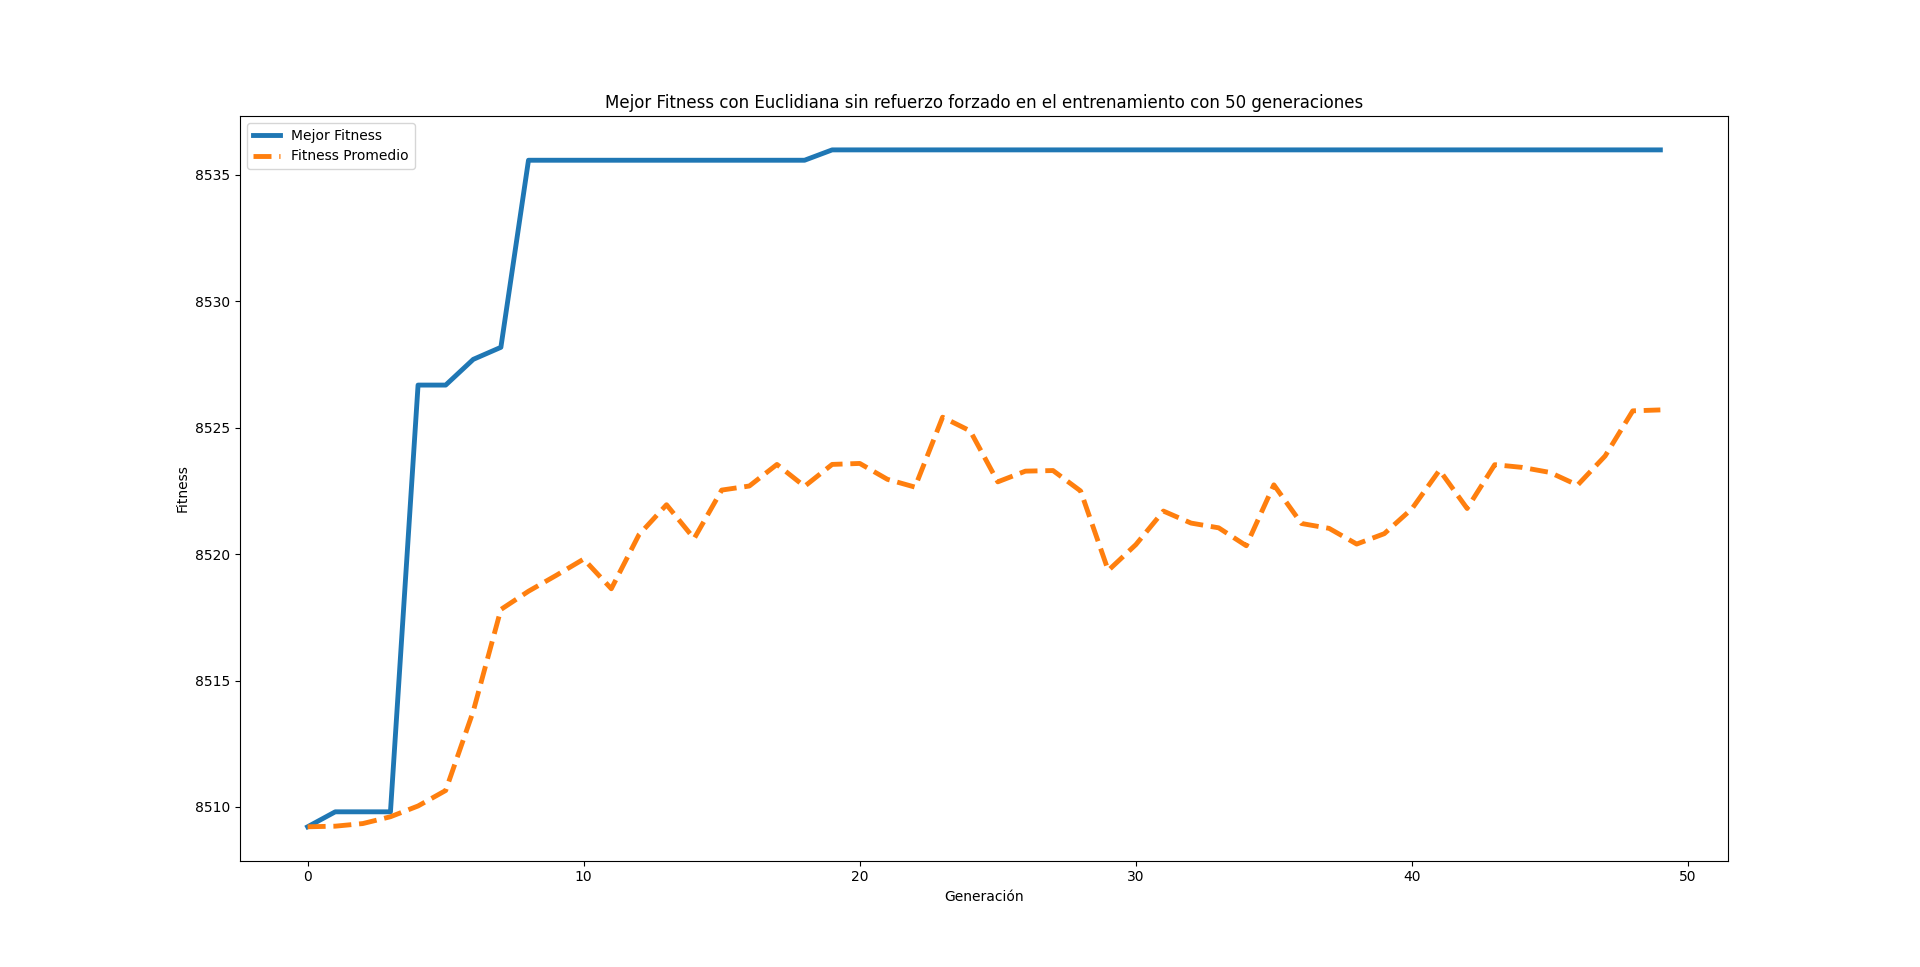
\includegraphics[width=0.9\linewidth]{Sin_Refuerzo_50Gen/Eucli_NoRef_50Gen.png}
    \caption{Mejor promedio fitness para la distancia Euclidiana sin la aplicación del Refuerzo forzado}
    \label{fig:no_refoice_eucli}
\end{figure}
por otra parte la desviación obtenida se puede observar en:
\begin{figure}[H]
    \centering
    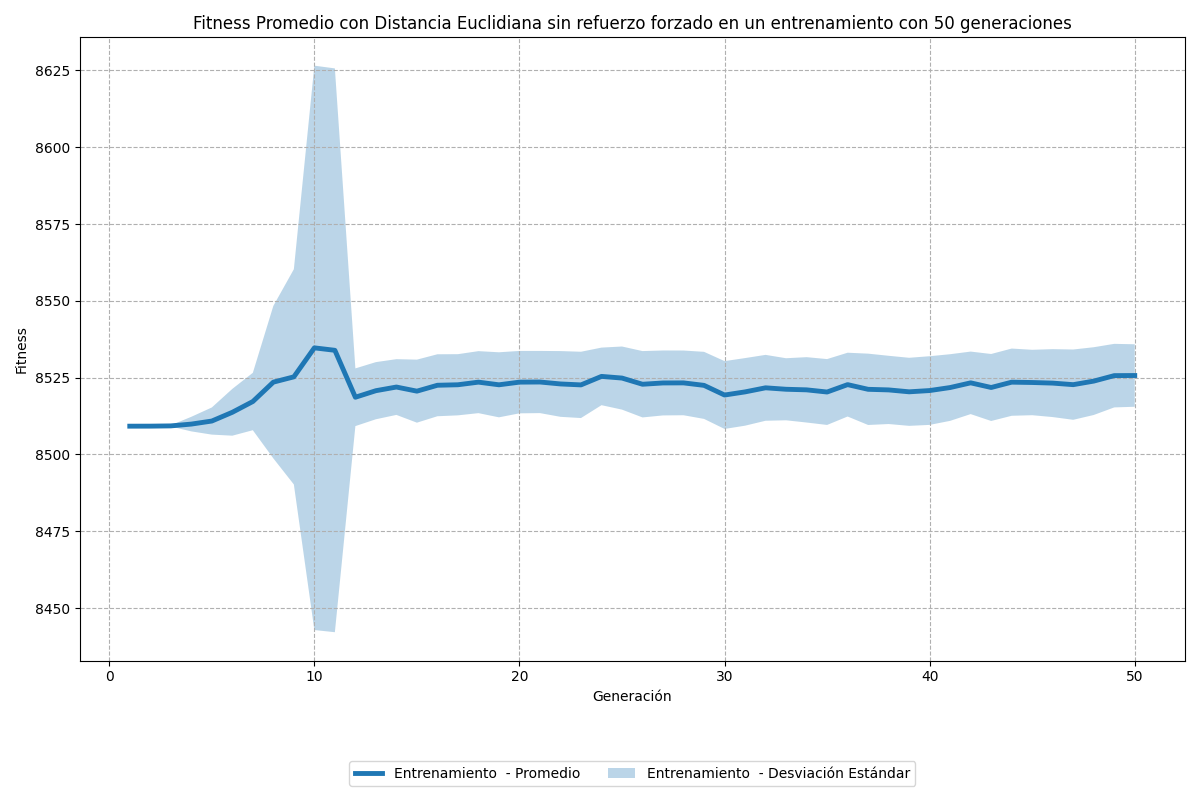
\includegraphics[width=0.9\linewidth]{Sin_Refuerzo_50Gen/Eucli_NoRef_50Gen_Sombra.png}
    \caption{Desviación y promedio fitness para la distancia Euclidiana sin la aplicación del Refuerzo forzado}
    \label{fig:no_refoice_eucli_desv}
\end{figure}
Donde la mayor desviación ocurrió en la generación número 10. Sin embargo luego de la decima generación la desviación disminuye, y juto con el primedio. Tanto la desviación como el promedio fitness se mantienen en un rango de 8525 puntos.

Implementando la distancia Manhattan el puntaje solo se diferencia en 1 de la distancia Euclidiana, con un puntaje de 8535
\begin{figure}[H]
    \centering
    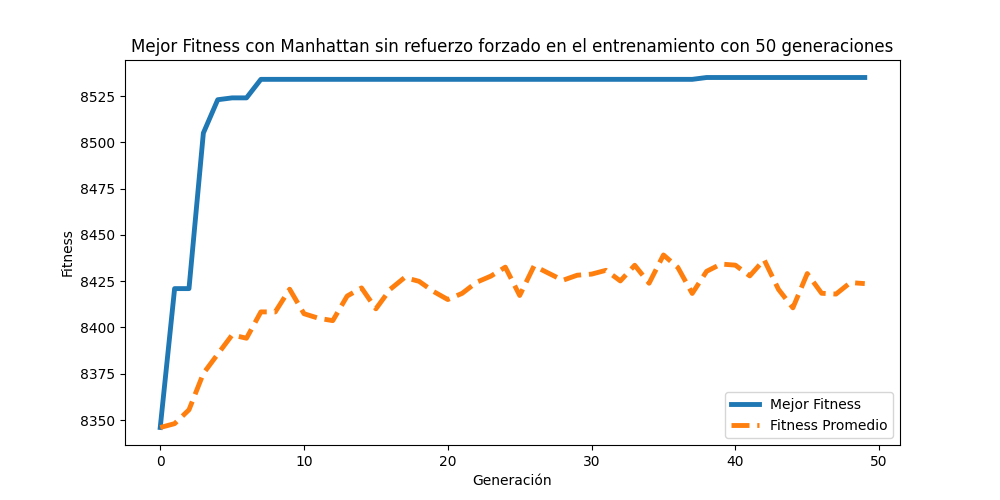
\includegraphics[width=0.9\linewidth]{Sin_Refuerzo_50Gen/Manh_NoRef_50Gen.png}
    \caption{Mejor promedio fitness para la distancia Euclidiana sin la aplicación del Refuerzo forzado}
    \label{fig:no_refoice_man}
\end{figure}
De igual manera, Manhattan también presenta la mayor desviación en la décima generación, sin embargo las desviacines superan levemente los 8500 puntos.
\begin{figure}[H]
    \centering
    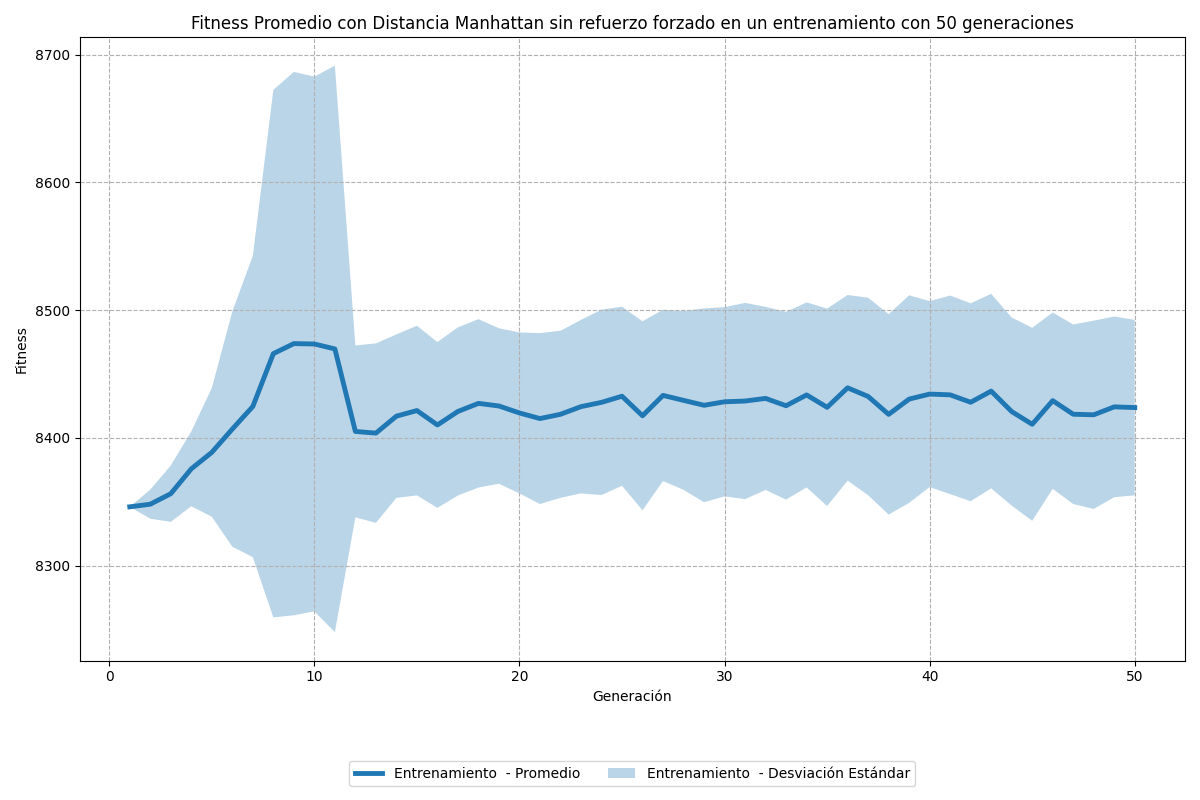
\includegraphics[width=0.8\linewidth]{Sin_Refuerzo_50Gen/Manh_NoRef_50Gen_Sombra.png}
    \caption{Desviación y promedio fitness para la distancia Manhattan sin la aplicación del Refuerzo forzado}
    \label{fig:no_refoice_man_desv}
\end{figure}

Por ultimo, en esta sección la distancia de Chebyshev presentó los mejores resultados, con un puntaje fitness máximo obtenido de 9885, y una desviación que ronda los 8800 puntos.
\begin{figure}[H]
    \centering
    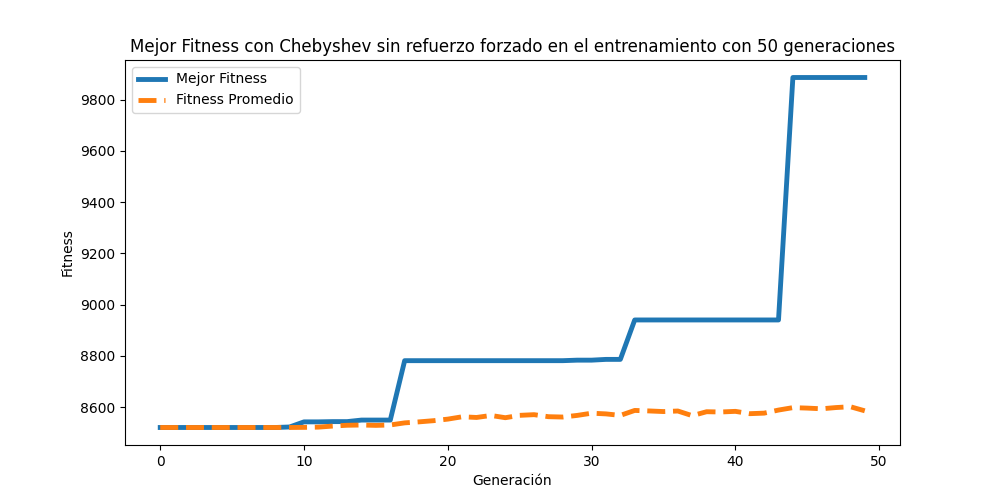
\includegraphics[width=1\linewidth]{Sin_Refuerzo_50Gen/Cheby_NoRef_50Gen.png}
    \caption{Mejor promedio fitness para la distancia Chebyshev sin la aplicación del Refuerzo forzado}
    \label{fig:no_refoice_chy}
\end{figure}
\begin{figure}[H]
    \centering
    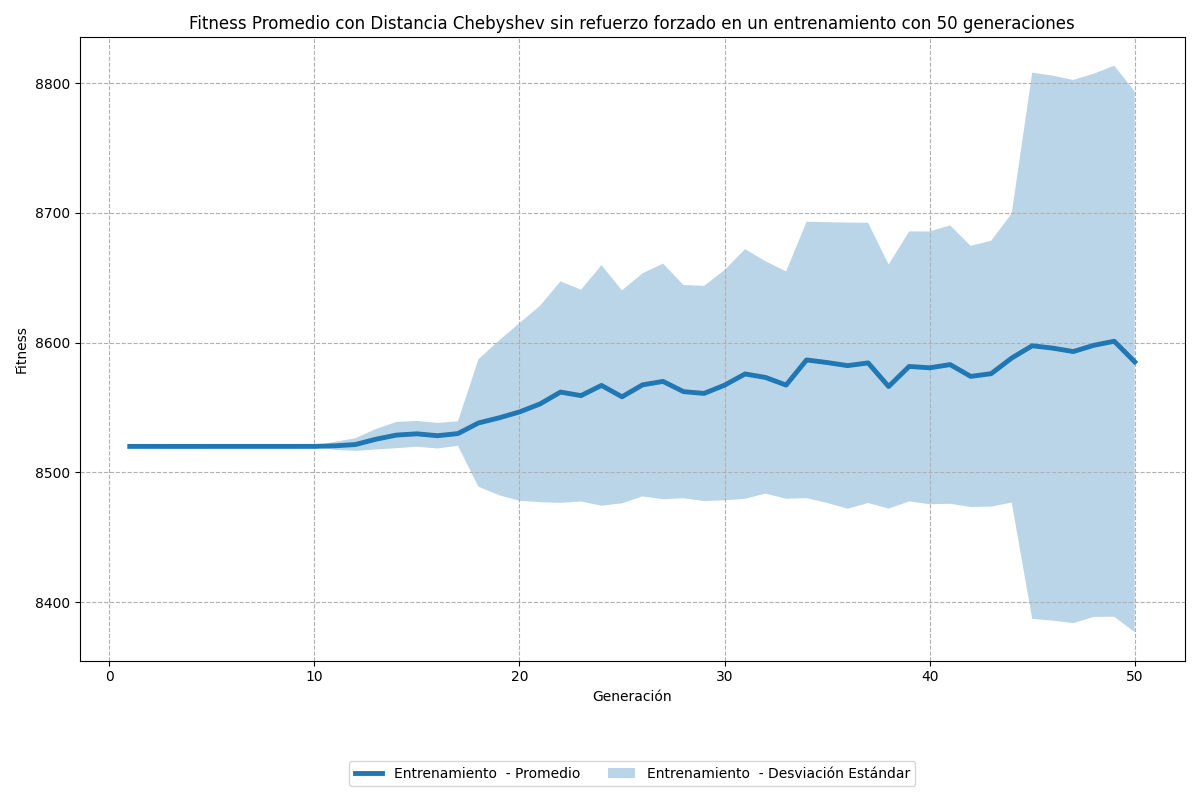
\includegraphics[width=0.9\linewidth]{Sin_Refuerzo_50Gen/Cheby_NoRef_50Gen_Sombra.png}
    \caption{Desviación y promedio fitness para la distancia Chebyshev sin la aplicación del Refuerzo forzado}
    \label{fig:no_refoice_chy_desv}
\end{figure}
Dentro de las características de esta simulación, apartir de la genreación 40, el fitness tuvo un incremento por encima de los 600 puntos, la desviación a partir de esta genración incrementó en un rango de 100 puttos. El promedio fitness empezó un incremento gradual desde la genración numero 15. 

\subsection{Simulaciones de 50 generaciones realizadas en el segundo mapa con el Refuerzo Forzado}
Se realizaron 5 simulaciones de 50 genraciónes para cada sistema de recompensas en el segundo mapa ver figura \ref{fig:mapa2}, Euclidiano, Manhattan y Chebyshev. Con los datos recopilados de estas simulaciones, se analizan las gráficas generales, y basándose en los resultados previos se hace una descripción
\subsubsection{Distancia Euclidiana}
La gráfica general obtenida después de cada entrenamiento para la distancia Euclidiana es:
\begin{figure}[H]
    \centering
    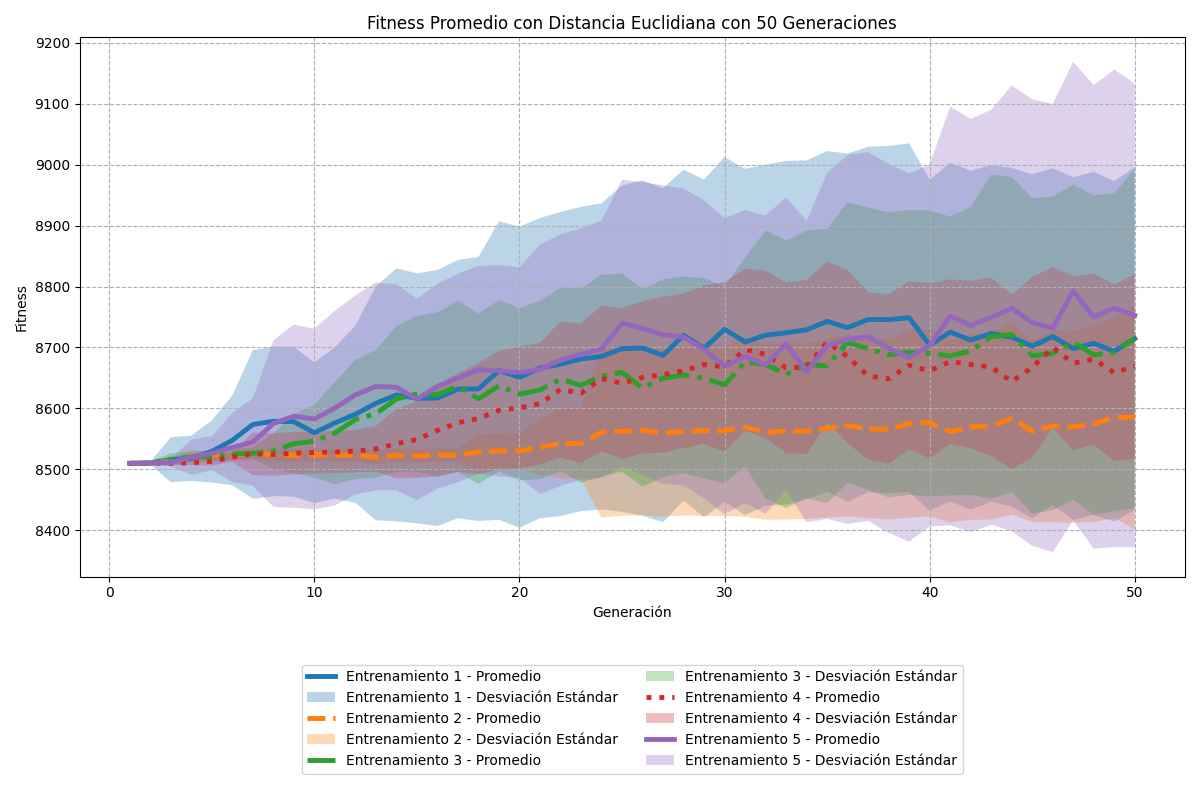
\includegraphics[width=0.9\linewidth]{Euclidiana/Mapa2/Fitness_Prrm_Map2_Eucli_50Gen.png}
    \caption{Gráfica de promedios fitness generales y desviaciones en cada entrenamiento para la distancia Euclidiana correspondiente a una generación de 50 y el segundo mapa}
    \label{fig:eucli_mapa2}
\end{figure}
El mejor fitness obtenido es de 9684, por el tercer y quinto entrenamiento. El quito entrenamiento en comparación con el tercero presenta una desviación que supera los 9100 puntos, por otra parte el tercer entrenamento no supera los 9000 puntos en desviación, quedandose incluso por debajo del primer entrenamiento. El primer entrenamiento obtuvo un fitness de 9456 puntos, seguido del segundo con 9443, pot último el menor fitness fue obtenido por el cuarto entrenamiento con 8933 puntos (Fig. \ref{fig:eucli_1_50_m2} hasta \ref{fig:eucli_5_50_m2})



\subsubsection{Distancia Manhattan}
La gráfica general obtenida después de cada entrenamiento para la distancia Manhattan es:
\begin{figure}[H]
    \centering
    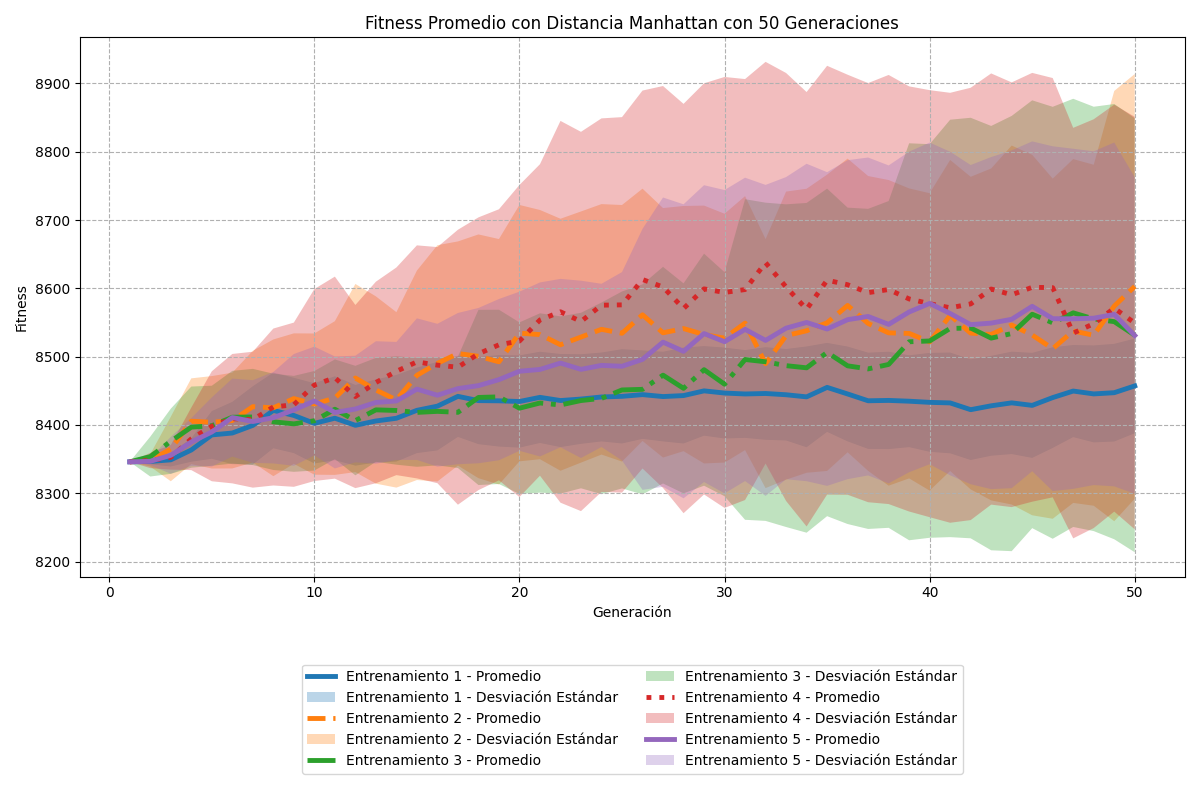
\includegraphics[width=0.9\linewidth]{Manhattan/Mapa2/Fitness_Prom_Map2_Manh_50Gen.png}
    \caption{Gráfica de promedios fitness generales y desviaciones en cada entrenamiento para la distancia Manhattan correspondiente a una generación de 50 y el segundo mapa}
    \label{fig:man_mapa_2}
\end{figure}

Para la distancia Manhattan el fitness más alto obtenido en estas simulaciones realizadas para es para el entrenamiento numero 2, con un puntaje máximo de 9890 y una desviación que supera los 8900 puntos. Además obvtuvo un incremento en el fitness promedio a partir de la genración 47. Con un fitness maximo de 9679, los entenamientos 4 y 3 obtuvieron los siguiente puntajes más altos. El cuarto entrenamiento empezó a disminuir su fitness promedio a partir de la genración 30, mientras que el tercer entrenamiento mantuvo un fitness ascendente. El quinnto y primer entrenamiento obtuvieron los puntajes mas bajos, con 9507 y 8532 respectivamente. Las desviaciones presentadas por el quinto entrenamiento superan los 8800 puntos, mientras que el primer entrenamiento no pasa de los 8550 puntos (Fig. \ref{fig:manh_1_50_m2} hasta \ref{fig:manh_5_50_sombra_m2})

\subsubsection{Distancia Chebyshev}
La gráfica general obtenida después de cada entrenamiento para la distancia Chebyshev es:
\begin{figure}[H]
    \centering
    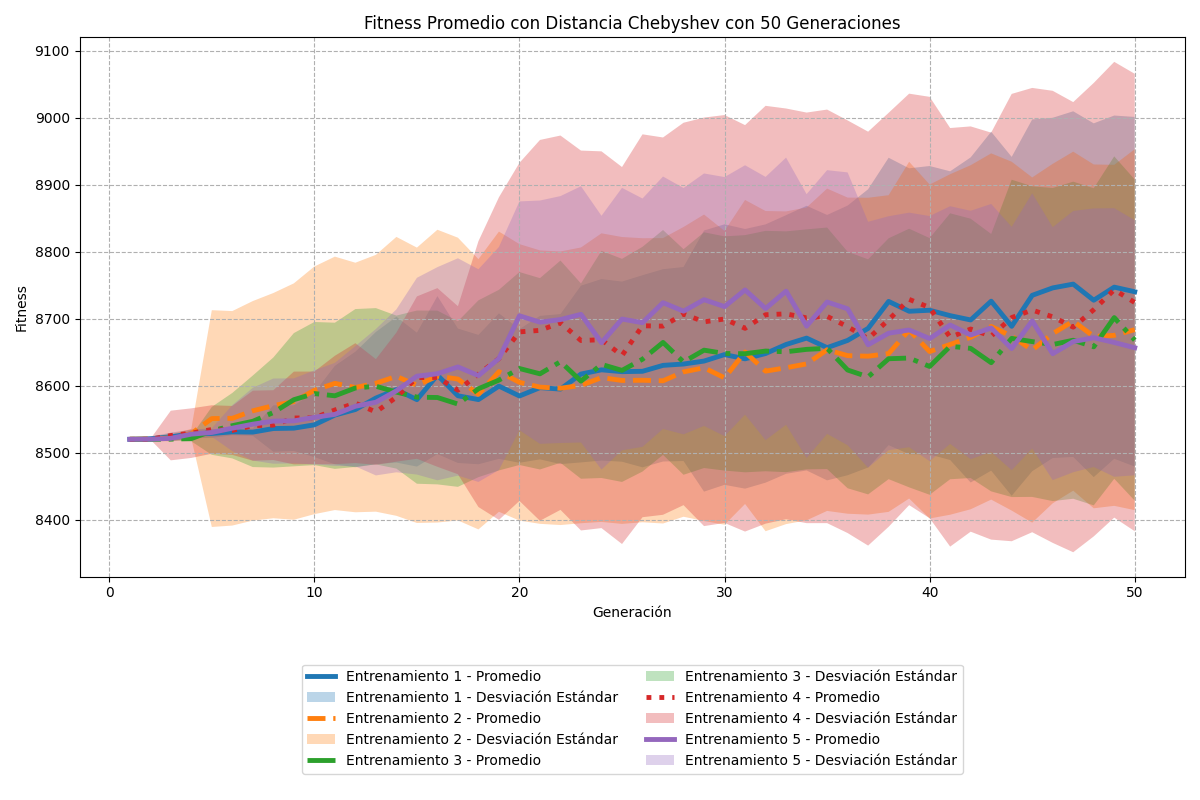
\includegraphics[width=0.9\linewidth]{Chebyshev/Mapa2/Fitness_Prom_Map2_Cheby_50Gen.png}
    \caption{Gráfica de promedios fitness generales y desviaciones en cada entrenamiento para la distancia Chebyshev correspondiente a una generación de 50 y el segundo mapa}
    \label{fig:chy_mapa_2}
\end{figure}
El entrenamiento que mayor fitness obtuvo en esta sección corresponde al cuarto entrenamiento con un puntaje de 9683, con una desviación que se acerca a los 9100 puttos. El segundo entrenamiento obtuvo el segundo mejor puntaje con 9671, con una desviación que no supera los 9000 puntos, sin embargo una característica particular de este entenamiento es que no posee desviaciones elevadas hasta la cuarta genración, sin embargo a partir de la generación numero 5, la desviacón se despira a los 8700 puntos hata llegar de forma gradual a los 8900. El entrenamiento numero 3 y 1 obtuvieron un puntaje fitness muy cercano entre ellos, solo con una diferencia de tres puntos. Para el tercer entrenamiento el fitness maximo obtenido es de 9764, mientras que para el primero fue de 9571 además de poseer una desvición mayor. Por último el peor fitness obtenido lo obtuvo el entrenamietno numero 5 con 8985 puntos y un decrecisimiento en la desviación a partir de la genración 30 (Fig. \ref{fig:cheb_1_50_m2} hasta \ref{fig:cheb_5_50_sombra_m2}).

\section{Conclusiones}
La implementación de la librería NEAT para un vehículo autónomo permitió analizar distintos aspectos del aprendizaje y desempeño del agente en diversos entornos. En este caso se realizaron dos pruebas, el entorno podría encontraba libre de obstáculos, mientras que en la otra se añadió un bloqueo de ruta. Se observó que el agente mostró un mejor rendimiento en el entorno libre de obstáculos, en comparación del entorno con la ruta bloqueada. Al agente le tomaba más generaciones aprender en comparación cuándo algunas de las vías era obstruida. En cuanto a las métricas de distancia, la distancia Chebyshev demostró ser más óptima que la Manhattan y Euclidiana en entornos libres de obstáculos. Sin embargo, en escenarios con obstáculos, la distancia Euclidiana ofreció un mejor desempeño que las demás obteniendo un alto valor fitness. La distancia Euclidiana aumentaba al igual que la de Chebyshev con el pasar de las generaciones, sin embargo la distancia Manhattan obtuvo su mayor fitness con una generación de 30. Con los datos obtenidos en la sección de resultados, se puede que puede concluir que para la distancia Manhattan y Chebyshev con 30 generaciones ya se obtienen unos excelentes puntajes, ya que para Chebyshev las simulaciones realizadas con 50 generaciones solo le aumentaron en dos puntos. 

Por otro lado, la implementación del refuerzo forzado generó mejoras importantes, ya que disminuyó el tiempo requerido para que el agente alcanzara un fitness significativo. Además, permitiendo que el agente aprendiera a girar en pocas generaciones. Por otra parte sin la aplicación del refuerzo forzado, el agente no lograba obtener fitness altos, lo que se traduce en un aprendizaje más lento y menos eficiente. Sin embargo la distancia de Chebyshev demostró ser las más eficiente sin la aplicación del refuerzo forzado, obteniendo un fitness de 9885, superando a la Euclidiana y Manhattan. 
\printbibliography
\end{document}